\documentclass[11pt,a4paper]{article}
% Comprehensive end-evaluation report. Compiles with Tectonic/XeLaTeX (tested) and pdflatex + bibtex (untested here).
% Sources are ASCII-only. Every result value comes from macros and tables written by the code
% (docs/nine_crop/generated/: numbers9.tex, numbers_india.tex, numbers_report.tex, tab_*.tex).
\usepackage{iftex}
\ifPDFTeX
  \usepackage[utf8]{inputenc}
  \usepackage[T1]{fontenc}
\fi
\usepackage{lmodern}
\usepackage[margin=2.3cm]{geometry}
% shared packages, notation and generated numbers for the end-evaluation report, slides and appendix
\usepackage{amsmath,amssymb}
\usepackage{booktabs}
\usepackage{graphicx}
\usepackage{siunitx}
\usepackage{xcolor}
\usepackage{adjustbox}
\makeatletter
\providecommand{\input@path}{}
\g@addto@macro\input@path{{.}{docs/}{./docs/}{../docs/}}
\makeatother
\graphicspath{{../figures/nine_crop/}{../figures/four_crop/}{figures/nine_crop/}}
% generated by code/19_endeval_tex.py -- do not edit
\newcommand{\nPairs}{59}
\newcommand{\nCountries}{20}
\newcommand{\nCrops}{9}
\newcommand{\orderEq}{Wheat $>$ Maize $>$ Common bean $>$ Soybean $>$ Rapeseed-mustard $>$ Chickpea $>$ Rice $>$ Lentil $>$ Groundnut}
\newcommand{\topEq}{Wheat}
\newcommand{\secondEq}{Maize}
\newcommand{\lastEq}{Groundnut}
\newcommand{\topEqValue}{0.0563}
\newcommand{\secondEqValue}{0.0297}
\newcommand{\orderPw}{Wheat $>$ Common bean $>$ Chickpea $>$ Rapeseed-mustard $>$ Soybean $>$ Maize $>$ Lentil $>$ Groundnut $>$ Rice}
\newcommand{\topPw}{Wheat}
\newcommand{\secondPw}{Common bean}
\newcommand{\lastPw}{Rice}
\newcommand{\topPwValue}{0.0696}
\newcommand{\secondPwValue}{0.0233}
\newcommand{\topPairA}{wheat--Russia}
\newcommand{\topPairAValue}{0.1315}
\newcommand{\topPairB}{maize--South Africa}
\newcommand{\topPairBValue}{0.1237}
\newcommand{\topPairC}{wheat--USA}
\newcommand{\topPairCValue}{0.0903}
\newcommand{\topPairD}{wheat--India}
\newcommand{\topPairDValue}{0.0676}
\newcommand{\topPairE}{common bean--Brazil}
\newcommand{\topPairEValue}{0.0459}
\newcommand{\topPairF}{common bean--Tanzania}
\newcommand{\topPairFValue}{0.0357}
\newcommand{\refHeatPair}{common bean--India}
\newcommand{\refHeat}{5.046}
\newcommand{\refWaterPair}{chickpea--India}
\newcommand{\refWater}{0.789}
\newcommand{\refImpPair}{rice--Bangladesh}
\newcommand{\refImp}{0.421}
\newcommand{\groupOrder}{Cereals $>$ Pulses $>$ Oilseeds}
\newcommand{\nDivUnits}{21}
\newcommand{\wheatTopZinc}{16}
\newcommand{\wheatTopIron}{15}
\newcommand{\wheatTopProtein}{9}
\newcommand{\wheatTopKcal}{14}
\newcommand{\maizeSAkcal}{22}
\newcommand{\maizeSArainfed}{89}
\newcommand{\maizeSAEwater}{0.46}
\newcommand{\maizeUAEwater}{0.61}
\newcommand{\maizeFoodUSA}{1}
\newcommand{\maizeFoodChina}{3}
\newcommand{\maizeFoodSA}{40}
\newcommand{\futHeatShare}{72}
\newcommand{\futWaterShare}{28}
\newcommand{\nPairsDown}{14}
\newcommand{\nPairsDownWaterOnly}{14}
\newcommand{\futOrderEq}{Wheat $>$ Maize $>$ Common bean $>$ Rapeseed-mustard $>$ Soybean $>$ Chickpea $>$ Rice $>$ Lentil $>$ Groundnut}
\newcommand{\histOrderEq}{Wheat $>$ Maize $>$ Common bean $>$ Soybean $>$ Rapeseed-mustard $>$ Chickpea $>$ Rice $>$ Groundnut $>$ Lentil}
\newcommand{\futOrderPw}{Wheat $>$ Common bean $>$ Chickpea $>$ Rapeseed-mustard $>$ Soybean $>$ Maize $>$ Lentil $>$ Groundnut $>$ Rice}
\newcommand{\nPairsUp}{40}
\newcommand{\nPairsExceedRef}{1}
\newcommand{\meanDTeff}{1.9}
\newcommand{\futTopPair}{wheat--Russia}
\newcommand{\futTopPairChange}{+0.0207}
\newcommand{\climCheckSameSign}{92}
\newcommand{\climCheckRho}{0.96}
\newcommand{\histReproMaxDiff}{4.3e-06}
\newcommand{\shockTopMar}{maize--South Africa}
\newcommand{\shockTopMarValue}{-0.53}
\newcommand{\shockTopKcal}{rice--Bangladesh}
\newcommand{\shockTopKcalValue}{-6.3}
\newcommand{\shockZeroMar}{40}
\newcommand{\shockN}{59}
\newcommand{\passOldN}{43}
\newcommand{\passOldPos}{17}
\newcommand{\passNewN}{49}
\newcommand{\passNewPos}{5}
\newcommand{\nIronShort}{7}
\newcommand{\nIronShortAlt}{0}
\newcommand{\nZincShort}{0}
\newcommand{\nZincShortAlt}{0}
\newcommand{\nAdqCountries}{20}
\newcommand{\futYieldWorst}{Common bean}
\newcommand{\futYieldWorstValue}{-17.8}
\newcommand{\futNutTopPair}{common bean--Brazil}
\newcommand{\futNutTopMar}{-0.66}
\newcommand{\corrLitEmp}{-0.04}
\newcommand{\robN}{184}
\newcommand{\robTopAll}{178}
\newcommand{\robTopFfour}{44}
\newcommand{\robNFfour}{46}
\newcommand{\mcTop}{Wheat}
\newcommand{\mcTopShare}{92.0}
\newcommand{\mcSecond}{Maize}
\newcommand{\mcSecondShare}{6.0}
\newcommand{\zhaoRhoFfour}{+0.6}
\newcommand{\zhaoRhoClimate}{+0.8}
\newcommand{\shockRho}{+0.35}
\newcommand{\shockP}{0.00}
\newcommand{\shockNpairs}{59}
\newcommand{\oosMedian}{0.33}
\newcommand{\oosPos}{28}
\newcommand{\oosN}{35}
\newcommand{\presentHeatShare}{9}
\newcommand{\presentWaterShare}{91}
\newcommand{\nTopSevenWater}{7}
\newcommand{\empHeatDetected}{22}
\newcommand{\empHeatCountry}{8}
\newcommand{\empN}{59}
\newcommand{\litN}{12}
\newcommand{\litAgree}{7}
\newcommand{\litDiffer}{2}
\newcommand{\litPartial}{1}
\newcommand{\litOther}{2}
\newcommand{\orderMidEq}{Wheat $>$ Maize $>$ Soybean $>$ Rice}
\newcommand{\orderOrigMidEq}{Wheat $>$ Maize $>$ Soybean $>$ Rice}
\newcommand{\orderMidPw}{Wheat $>$ Soybean $>$ Maize $>$ Rice}
\newcommand{\orderOrigMidPw}{Wheat $>$ Soybean $>$ Maize $>$ Rice}
\newcommand{\orderFourEq}{Wheat $>$ Maize $>$ Soybean $>$ Rice}
\newcommand{\orderOrigFourEq}{Wheat $>$ Maize $>$ Soybean $>$ Rice}
\newcommand{\orderFourPw}{Wheat $>$ Soybean $>$ Maize $>$ Rice}
\newcommand{\orderOrigFourPw}{Wheat $>$ Soybean $>$ Maize $>$ Rice}
\newcommand{\orderNineEq}{Wheat $>$ Maize $>$ Bean $>$ Soybean $>$ Rapeseed $>$ Chickpea $>$ Rice $>$ Lentil $>$ Groundnut}
\newcommand{\orderOrigNineEq}{Wheat $>$ Maize $>$ Soybean $>$ Rice}
\newcommand{\orderNinePw}{Wheat $>$ Bean $>$ Chickpea $>$ Rapeseed $>$ Soybean $>$ Maize $>$ Lentil $>$ Groundnut $>$ Rice}
\newcommand{\orderOrigNinePw}{Wheat $>$ Soybean $>$ Maize $>$ Rice}
\newcommand{\litTopPair}{wheat--Russia}
\newcommand{\litTopValue}{0.2099}
\newcommand{\litSecondPair}{wheat--India}
\newcommand{\litSecondValue}{0.2076}
\newcommand{\litRatioMedian}{1.76}
\newcommand{\exFourLheatc}{0.580}
\newcommand{\exFourmaxLheat}{0.580}
\newcommand{\exFourEheat}{1.000}
\newcommand{\exFourLwater}{0.178}
\newcommand{\exFourmaxLwater}{0.546}
\newcommand{\exFourEwater}{0.327}
\newcommand{\exFoursTpc}{0.100}
\newcommand{\exFourmaxsT}{0.200}
\newcommand{\exFourSheat}{0.500}
\newcommand{\exFourKy}{1.10}
\newcommand{\exFourmaxKy}{1.25}
\newcommand{\exFourSwater}{0.880}
\newcommand{\exFourI}{0.222}
\newcommand{\exFourmaxI}{0.421}
\newcommand{\exFourInorm}{0.527}
\newcommand{\exFourFFourpipeline}{0.2076}
\newcommand{\exNineLheatc}{0.580}
\newcommand{\exNinemaxLheat}{5.046}
\newcommand{\exNineEheat}{0.115}
\newcommand{\exNineLwater}{0.178}
\newcommand{\exNinemaxLwater}{0.789}
\newcommand{\exNineEwater}{0.226}
\newcommand{\exNinesTpc}{0.100}
\newcommand{\exNinemaxsT}{0.200}
\newcommand{\exNineSheat}{0.500}
\newcommand{\exNineKy}{1.10}
\newcommand{\exNinemaxKy}{1.25}
\newcommand{\exNineSwater}{0.880}
\newcommand{\exNineI}{0.222}
\newcommand{\exNinemaxI}{0.421}
\newcommand{\exNineInorm}{0.527}
\newcommand{\exNineFFourpipeline}{0.0676}

\InputIfFileExists{nine_crop/generated/numbers_india.tex}{}{}

\definecolor{ink}{HTML}{222222}
\definecolor{muted}{HTML}{6B6B6B}
\definecolor{paddy}{HTML}{1F4E3D}
\definecolor{grain}{HTML}{C8961A}
\definecolor{clay}{HTML}{B5523B}
\definecolor{cereal}{HTML}{2A78D6}
\definecolor{pulse}{HTML}{EB6834}
\definecolor{oilseed}{HTML}{1BAF7A}
\newcommand{\Teff}{\ensuremath{T_{\mathrm{eff}}}}
\newcommand{\Tcrit}{\ensuremath{T_{\mathrm{crit}}}}
\newcommand{\ETc}{\ensuremath{\mathrm{ET_c}}}
\newcommand{\ETo}{\ensuremath{\mathrm{ET_0}}}
\newcommand{\Fd}{\ensuremath{\mathrm{F4}}}

\InputIfFileExists{nine_crop/generated/numbers_report.tex}{}{}
\usepackage[round]{natbib}
\usepackage{float}
\usepackage{longtable}
\usepackage{array}
\usepackage{enumitem}
\usepackage{caption}
\captionsetup{font=small,labelfont=bf}
\usepackage[nottoc]{tocbibind}
\usepackage{hyperref}
\hypersetup{colorlinks=true,linkcolor=paddy,citecolor=paddy,urlcolor=paddy,bookmarksnumbered=true,
  pdftitle={Climate Change and Nutritional Security: Which Crops Are Most Vulnerable?},pdfauthor={Mahtele, Patel, Puri, Lohare}}
\bibliographystyle{plainnat}
\numberwithin{equation}{section}
\setlength{\parskip}{0.35em}
\setlist{itemsep=0.15em,topsep=0.3em}
\setcounter{tocdepth}{2}
\usepackage{seqsplit}
\DeclareRobustCommand{\file}[1]{\texttt{\seqsplit{#1}}}
% L{f}: ragged column of width f x line width (used by the generated longtables)
\newcolumntype{L}[1]{>{\raggedright\arraybackslash}p{\dimexpr#1\linewidth-2\tabcolsep\relax}}

\title{Climate Change and Nutritional Security:\\ Which Crops Are Most Vulnerable?\\[0.4em]
\large A Climate--Nutrition Vulnerability Index for nine crops, present and 2041--2060\\[0.2em]
\normalsize End-evaluation report, Earth 616 (Environmental Science)}
\author{Arpit Mahtele \and Dev Patel \and Navey Puri \and Shreyash Lohare}
\date{November 2026}

\begin{document}
\maketitle
\thispagestyle{empty}

\begin{abstract}
\noindent\textbf{Questions.} Which food crops are most vulnerable to observed and projected heat and water stress,
once we count how much people depend on them for nutrients? And if such a crop's yield falls, what happens to a
country's nutrient supply?

\noindent\textbf{Method.} The Climate--Nutrition Vulnerability Index pairs each stress with its own crop response:
$\Fd = \tfrac12(E_{\text{heat}}S_T + E_{\text{water}}S_P)\,\tilde I$, from the observed 2001--2024 stress level
($E$), literature sensitivity (yield lost per degree above a threshold, and FAO's $K_y$; $S$) and the crop's mean
share of national energy, protein, fat, zinc and iron supply ($\tilde I$). It covers nine crops in \nPairs\
crop--country pairs and three periods: 2001--2024, 1971--2000, and 2041--2060 under one climate model (MRI-ESM2-0,
SSP2-4.5) with a fixed normalisation. Nutrient consequences are computed for a standard 10\% yield loss and, as a
\emph{conditional screening estimate}, for the projected climate-driven yield change.

\noindent\textbf{Findings.}
\begin{itemize}
\item \topEq\ is the most vulnerable crop under both country weightings, in \robTopFfour\ of \robNFfour\ robustness
rankings and in \mcTopShare\% of random weightings. The order below first place is not stable.
\item Water deficit dominates today's scores (\presentWaterShare\%); heat dominates the projected increase. The
flowering-season effective temperature rises by \meanDTeff\,\si{\celsius} and the score rises in \nPairsUp\ of
\nPairs\ pairs.
\item Iron is the nutrient closest to shortfall (\nIronShort\ of \nAdqCountries\ countries under the main
requirement, none under a 15\%-bioavailability requirement).
\item India's ranking is led by wheat, chickpea and common bean; the nine crops supply \shareNewKcal\% of its energy
and \shareNewIron\% of its iron. Hyderabad's rice-based diet coexists with anaemia in \hydAnaemNPW\% of non-pregnant
women in the district; its nutritional risk is more structural than climatic.
\end{itemize}

\noindent\textbf{Four extensions test the foundations.}
\begin{itemize}
\item \textbf{Parameters.} Of \parNRows\ audited parameter rows, the rice and rapeseed heat slopes are unsupported.
Wheat is still first among the seven crops with supported parameters; rice and rapeseed cannot be placed.
\item \textbf{Literature.} \litNRows\ rows from \litNStudies\ publications cover all nine crops; direction agrees where
studies are most comparable and differs where they include CO$_2$ fertilisation or adaptation.
\item \textbf{CO$_2$ and quality.} As a stress test with partial coverage (not a forecast), lower grain concentrations
cut India's zinc supply by \cotwoIndQualZincAbs\% and, with the climate yield loss, by \cotwoIndCombZincAbs\%.
\item \textbf{Diversity.} Losing part of a dominant staple lowers supply but can raise the effective number of food
sources, so diversity must be read with adequacy.
\end{itemize}

\noindent\textbf{What the evidence supports.} The baseline results were regenerated from checksummed raw inputs and are
identical to the previous outputs; \checksPassed\ of \checksN\ consistency checks and \extChecksPassed\ of
\extChecksN\ extension checks pass. This shows that the numbers follow from the stated method, not that the method is
valid. Several parameters are fits or proxies, literature and empirical future yield responses disagree for about half
of the pairs, and validation against yield shocks shows an association only.
\end{abstract}


\clearpage
\tableofcontents
\clearpage
\listoffigures
\listoftables
\clearpage

\section{Introduction}\label{sec:intro}

\subsection{Problem and research questions}
Climate change affects nutrition through two channels. The first is how much of each crop is produced. The
second is what that crop contributes to diets. A crop matters for nutrition security when three things
coincide: its growing areas are under heat or water stress, its yield falls quickly under that stress, and many
people depend on it for energy or micronutrients. This report asks:
\begin{enumerate}[label=\textbf{RQ\arabic*}]
\item Which of nine major food crops (three cereals, three pulses, three oilseeds) is most vulnerable to
observed (2001--2024) and projected (2041--2060) heat and water stress, given its nutritional importance, and
does the answer differ between countries and crop groups?
\item If a crop's yield falls, by a standard amount or by the amount implied by the projected climate change,
what happens to a country's supply of energy, protein, fat, zinc and iron, and to its nutrient adequacy?
\item What does the index indicate for one place studied in more detail: India, Telangana and the city of
Hyderabad?
\item How well supported are the crop parameters, do published future-impact studies point the same way for each
crop, what does an elevated-CO$_2$ change in nutrient concentration add to the yield channel, and how do crop losses
change the diversity of a country's food sources? (Four research extensions, Sections~\ref{sec:parevidence}--\ref{sec:divloss}.)
\end{enumerate}

\subsection{Literature context}
\paragraph{Climate and yield.} The yield literature is large and quantitative.
\begin{itemize}
\item Four independent methods agree that each degree of global warming lowers global yields of wheat, rice,
maize and soybean by about 6.0, 3.2, 7.4 and 3.1\% without CO$_2$ fertilisation or adaptation \citep{zhao2017}.
\item Year-to-year climate variation explains about a third of global yield variability \citep{ray2015}.
\item Crop models project large regional losses under warming \citep{rosenzweig2014,jagermeyr2021}.
\item Statistical studies attribute part of the recent yield trend to warming \citep{lobell2007,lobell2011}.
\item Process studies locate most of the damage in the reproductive phase, where a few hot days above a crop
threshold reduce seed set \citep{jagadish2007,deryng2014,boote2005}.
\end{itemize}
These studies measure yield; they do not ask who eats the crop.

\paragraph{Climate and nutrition.} The nutrition literature has a different emphasis.
\begin{itemize}
\item Elevated CO$_2$ lowers zinc, iron and protein in C$_3$ grains and legumes \citep{myers2014,smith2018,zhu2018,beach2019}.
\item Diet-level work asks how environmental change alters food supply and diet quality
\citep{scheelbeek2018,nelson2018,medek2017}.
\item The diversity of national food supply is itself an indicator of nutritional resilience \citep{remans2014}.
\end{itemize}

\paragraph{Vulnerability indices.} These indices usually follow the IPCC framing of exposure, sensitivity and
adaptive capacity \citep{ipcc2022ch5}, and crop-suitability studies map where crops will remain viable
\citep{ramirez2017,rippke2016}.

\paragraph{The gap.} Yield losses, nutrient supply and vulnerability scores are reported on incompatible scales.
We found no reviewed study that ranks crops by combining their climatic exposure, their sensitivity and their
nutritional importance in one index.

\subsection{Contribution}
The project contributes:
\begin{itemize}
\item a transparent index that combines the three in one number per crop and country (Section~\ref{sec:index});
\item its application to nine crops in three groups, for the present, a historical baseline and a mid-century
future, with one processing chain and one normalisation reference (Section~\ref{sec:periods});
\item an accounting step from yield loss to national nutrient supply and adequacy (Section~\ref{sec:nutmethod});
\item a local reading of the results for India and Hyderabad, using official survey data at the resolutions
they are actually published (Section~\ref{sec:india});
\item a reproducible evidence trail: raw-data checksums, a complete pipeline, generated tables, and a parameter
ledger that labels every derived value and proxy (Section~\ref{sec:repro}, Appendix~\ref{app:ledger});
\item four research extensions that test the result rather than extend its claims: an audit of how well each
parameter is supported with an evidence-screened view (Section~\ref{sec:parevidence}); a coverage assessment of
published future-impact studies for all nine crops (Section~\ref{sec:futurelit}); an elevated-CO$_2$ nutrient-quality
stress test (Section~\ref{sec:co2}); and the diversity of national food supply after crop losses
(Section~\ref{sec:divloss}).
\end{itemize}
The index is a \emph{screening} tool. It shows where stress and dependence coincide. It does not forecast yields
or diets.

\paragraph{Framing.} The structure follows the IPCC AR4 vulnerability framing (exposure $\times$ sensitivity
$\times$ adaptive capacity), with adaptive capacity replaced by nutritional \emph{importance}. In AR5/AR6
vocabulary the index is closer to a risk index, in which the stress plays the role of hazard and nutrition is
what is exposed. The substitution is deliberate, because the project asks about nutrition security, not about
farmers' coping capacity. It also means the index is not a pure climate-impact measure.

\subsection{Relation to the mid-evaluation and how to read this report}
The mid-evaluation presented the method for four crops (rice, wheat, maize, soybean). Its deck, report, tables
and figures are frozen in \file{archive/mid\_evaluation/}, and no number from them is reused as a new result.
This report completes the commitments made then.
\begin{itemize}
\item The presented \emph{literature-only} sensitivity is now used everywhere. The mid-evaluation numbers had
used an average of literature and observed-yield sensitivity; that version survives only as a robustness test.
\item The analysis covers nine crops, the future period, the nutrition consequences, and robustness,
validation and literature comparison under the final configuration.
\end{itemize}

\paragraph{Where to find things.}
\begin{itemize}
\item \textbf{Method:} Sections~\ref{sec:scope}--\ref{sec:periods}, with symbols in Table~\ref{tab:symbols}.
\item \textbf{Worked examples:} Section~\ref{sec:worked}.
\item \textbf{Results:} Sections~\ref{sec:present}--\ref{sec:india}.
\item \textbf{Research extensions} (parameter evidence, future literature, CO$_2$ quality, diversity after losses):
Sections~\ref{sec:parevidence}--\ref{sec:divloss}.
\item \textbf{Robustness, validation and literature comparison:} Section~\ref{sec:checks}.
\item \textbf{Limitations and conclusions:} Sections~\ref{sec:limits}--\ref{sec:discussion}.
\item \textbf{Reproduction and audit:} Section~\ref{sec:repro}.
\item \textbf{Appendices:} the parameter and source ledger, full result tables, the record of corrections, and
the audit evidence.
\end{itemize}

Every number from our own results is a macro or table written by the code from the saved results
(\file{docs/nine\_crop/generated/}); no result is typed by hand. Numbers quoted from published studies are typed
from the sources recorded in the evidence files and carry a citation.

\section{Scope: crops, groups and countries}\label{sec:scope}

\subsection{Crops and groups}
The index covers nine crops in three predefined groups:
\begin{itemize}
\item \textbf{cereals}: wheat, rice, maize;
\item \textbf{pulses}: chickpea, lentil, common bean;
\item \textbf{oilseeds}: soybean, groundnut, rapeseed-mustard.
\end{itemize}
The groups were fixed before any result was computed. A group score is the simple mean of its three crops'
scores (Section~\ref{sec:aggregation}). It describes these three crops, not every cereal, pulse or oilseed.

Each crop must be identified in five datasets: FAOSTAT production, the SPAM crop map, the Sacks calendar, the FAO
food balance sheets and the food composition table. The identifiers are listed in Table~\ref{tab:cropmap}
(Section~\ref{sec:data}). Three definitions need explanation.
\begin{itemize}
\item \textbf{Rapeseed-mustard} is a single item definition used everywhere: FAOSTAT ``Rape or colza seed'' (India
reports its rapeseed-mustard here; the separate ``Mustard seed'' item is about 1\% of the total and is excluded),
SPAM \texttt{RAPE}, and the food-balance items ``Rape and Mustardseed'' and ``Rape and Mustard Oil''.
\item \textbf{Common bean} is FAOSTAT ``Beans, dry''. In India and Myanmar this item also contains tropical
\emph{Vigna} pulses, which are not \emph{Phaseolus vulgaris}. The bean heat parameter is therefore applied beyond
the species it was measured on (Appendix~\ref{app:ledger}).
\item \textbf{Chickpea and lentil} have production and crop-map entries of their own. The food balance sheets,
however, report them only inside the aggregate ``Pulses, Other and products''. Their food supply is taken from the
FAOSTAT Supply Utilization Accounts (Section~\ref{sec:fbsmap}).
\end{itemize}

\subsection{Country selection rule}\label{sec:panelrule}
Countries are chosen per crop by the rule presented at the mid-evaluation, applied unchanged. Production is the
FAOSTAT mean for 2020--2024.
\begin{enumerate}
\item The \textbf{core countries} USA, Brazil, India and China are included for every crop they produce.
\item \textbf{One European and one African country.} A country is used for all crops if it is among its
continent's top three producers of every crop. Otherwise each crop uses its continent's largest producer.
\item The crop's \textbf{world top-3 producers} are added.
\end{enumerate}
A core country enters a crop's panel only if FAOSTAT records production there in 2020--2024 \emph{and} SPAM~2010
maps crop area there. With nine crops, no European or African country is in its continent's top three for every
crop, so the rule's own fallback applies. This changes two of the original four-crop panels: rice uses Italy
instead of Russia, and maize uses Ukraine instead of Russia. Three combinations are excluded by the rule:
\begin{itemize}
\item Brazil for chickpea and for lentil (no production or no mapped area);
\item groundnut in Europe (no European production recorded).
\end{itemize}
The result is \nPairs\ crop--country pairs in \nCountries\ countries (Table~\ref{tab:panels}). The panels cover
between half and nine-tenths of world production of each crop. A panel is a sample of the main producing
systems, not a census, so a crop's score describes these countries only.

\begin{table}[H]\centering\small
\caption{Country panels (FAOSTAT production 2020--24; world rank order; $*$ = less than 0.5\% of world output).}\label{tab:panels}
\adjustbox{max width=\linewidth}{\begin{tabular}{lp{10.5cm}r}
\toprule
Crop & Countries (world rank order; * = <0.5\% of world output) & \% world \\
\midrule
Wheat & China, India, Russia, USA, Egypt, Brazil & 51 \\
Rice & China, India, Bangladesh, Brazil, USA, Nigeria, Italy* & 63 \\
Maize & USA, China, Brazil, India, Ukraine, South Africa & 70 \\
Chickpea & India, Australia, Turkey, Ethiopia, Russia, USA, China* & 89 \\
Lentil & Canada, India, Australia, USA, Russia, China, Ethiopia & 82 \\
Common bean & India, Brazil, Myanmar, Tanzania, China, USA, Belarus & 59 \\
Soybean & Brazil, USA, Argentina, China, India, Russia, South Africa & 90 \\
Groundnut & China, India, Nigeria, USA, Brazil & 67 \\
Rapeseed-mustard & Canada, China, India, France, USA, South Africa*, Brazil* & 61 \\
\bottomrule
\end{tabular}
}
\end{table}

\subsection{Periods}
\begin{itemize}
\item \textbf{Present:} 2001--2024, observed monthly climate.
\item \textbf{Historical baseline:} 1971--2000, observed.
\item \textbf{Future:} 2041--2060, one climate model (MRI-ESM2-0) under one scenario (SSP2-4.5).
\end{itemize}
Importance is fixed at the 2021--2023 food balance sheets in every period. Crop area, irrigation and calendars are
fixed at their 2010 maps. Sensitivity is fixed at its literature values.

\section{Data, versions and preprocessing}\label{sec:data}

\subsection{Raw inputs}
Table~\ref{tab:datasources} lists every raw dataset with its version, size and file date. The manifest
\file{docs/DATA\_MANIFEST.csv} records each of the \manifestFiles\ raw files (\manifestGB\,GB) with its SHA-256
checksum, so any later run can confirm that it uses exactly the same inputs (Section~\ref{sec:repro}). The files
come from two snapshots:
\begin{itemize}
\item the mid-evaluation snapshot (5 October 2026): climate, SPAM, the original calendars, FAOSTAT, USDA and
Natural Earth;
\item an end-evaluation snapshot (17 November 2026): the calendars of the new crops, the WorldClim normals and
CMIP6 files, the FAOSTAT Supply Utilization Accounts, the admin-1 boundaries and the Indian survey files.
\end{itemize}
FAOSTAT bulk files are revised over time, so the numbers are exactly reproducible only from these archived files.

{\scriptsize\begin{longtable}{L{0.275}L{0.131}L{0.137}L{0.191}rrL{0.096}}
\caption[Raw inputs]{Raw inputs (from \texttt{docs/DATA\_MANIFEST.csv}, which lists every file with its SHA-256 checksum).}\label{tab:datasources}\\
\toprule
Dataset & Version & Source & Used for & Files & MB & File date \\
\midrule\endfirsthead
\toprule
Dataset & Version & Source & Used for & Files & MB & File date \\
\midrule\endhead
\bottomrule\endfoot
WorldClim 2.1 monthly weather (CRU-TS 4.09 downscaled), 10$'$; elevation; 1970--2000 precipitation normals & CRU-TS 4.09; WorldClim 2.1 & \citet{fick2017,harris2020} & monthly precipitation 1970--2024; elevation & 8 & 1{,}209 & 2026-10-05 \\
WorldClim 2.1 monthly maximum temperature, 10$'$ & CRU-TS 4.09 & \citet{fick2017,harris2020} & $T_{\max}$ 1970--2024 & 6 & 748 & 2026-10-05 \\
WorldClim 2.1 monthly minimum temperature, 10$'$ & CRU-TS 4.09 & \citet{fick2017,harris2020} & $T_{\min}$ 1970--2024 & 6 & 725 & 2026-10-05 \\
WorldClim 2.1 monthly normals $T_{\max}$, $T_{\min}$, 10$'$ & 1970--2000 & \citet{fick2017} & baseline of the change factors & 2 & 75 & 2026-11-17 \\
WorldClim 2.1 CMIP6 downscaled climatology, MRI-ESM2-0, SSP2-4.5, 10$'$ & 2041--2060 & \citet{wcmip6} & future change factors & 3 & 54 & 2026-11-17 \\
SPAM 2010 harvested area (all, irrigated, rainfed), 5$'$ & v2.0 & \citet{spam2010} & crop area weights, rainfed share & 2 & 144 & 2026-10-05 \\
Crop calendar dataset (planting, harvest) & Sacks et al.\ 2010 & \citet{sacks2010} & growing season and flowering window & 20 & 70 & 2026-10-05 / 2026-11-17 \\
FAOSTAT bulk: crop production (QCL); Food Balances 2010-- and --2013; Food Security indicators & bulk files of 5 Oct 2026 & \citet{faostat} & panels, yields, nutrient supply, energy requirement & 4 & 163 & 2026-10-05 \\
FAOSTAT Supply Utilization Accounts, crops & bulk file of 17 Nov 2026 & \citet{faosua} & chickpea and lentil supply & 1 & 89 & 2026-11-17 \\
USDA FoodData Central, SR Legacy & April 2018 release & \citet{usda2019} & zinc and iron per 100 g & 1 & 6 & 2026-10-05 \\
Natural Earth admin-0 countries, 1:50m & -- & Natural Earth (public domain) & country masks, continents & 1 & 1 & 2026-10-05 \\
Natural Earth admin-1 states/provinces, 1:10m & -- & Natural Earth (public domain) & Telangana mask & 1 & 15 & 2026-11-17 \\
K\"oppen--Geiger 1991--2020, 0.5\textdegree & Beck et al.\ 2023 & \citet{beck2018} & check of our K\"oppen groups & 1 & 0 & 2026-10-05 \\
Official India/Telangana/Hyderabad files: MoSPI HCES 2023--24, NSS 592 and 594, NFHS-5, CNNS, ICMR-NIN IFCT 2017, Telangana DES & see Appendix~\ref{app:indiasources} & Section~\ref{sec:india} & Hyderabad and Telangana analysis & 18 & 99 & 2026-11-17 \\
\end{longtable}}


\subsection{Gridded climate, crop area and calendars}
All gridded work is done on a 10 arc-minute global grid (about 18\,km at the equator).
\begin{itemize}
\item \textbf{Climate.} WorldClim~2.1 historical monthly weather (CRU-TS 4.09 downscaled) gives monthly
$T_{\max}$, $T_{\min}$ and precipitation $P$ for 1970--2024; $T_{\text{mean}} = (T_{\max}+T_{\min})/2$. Monthly data
cannot show individual hot days, a limitation discussed in Section~\ref{sec:limits}. In cell-months with no nearby
station, CRU-TS falls back to climatology, which weakens year-to-year rainfall variation in data-poor regions.
\item \textbf{Crop area.} SPAM~2010 harvested area (all, irrigated, rainfed; 5$'$) is summed to the 10$'$ grid. It
gives each cell's crop hectares $A_i$ and rainfed hectares $R_i$. Cells are assigned to countries with the
Natural Earth admin-0 boundaries.
\item \textbf{Calendars.} The Sacks et al.\ dataset gives planting and harvest days per cell; observed values are
used first and gap-filled values only as a fallback. Chickpea, lentil and rapeseed-mustard use a
\textbf{cool-season rule}, for three reasons:
  \begin{itemize}
  \item Sacks et al.\ have no chickpea or lentil calendar;
  \item their generic ``Pulses'' calendar is 95\% gap-filled in India;
  \item that calendar places these winter (rabi) crops in the monsoon season.
  \end{itemize}
  The rule takes the crop's own observed calendar where one exists (winter rapeseed in China, India and Europe),
  then the spring-wheat calendar where winters are cold (K\"oppen group D), then the wheat calendar elsewhere. This
  gives rabi sowing in South Asia, autumn sowing in Australia and spring sowing in Canada and Russia. The plain
  Sacks calendar is kept as a robustness test.
\item \textbf{Elevation and climate zones.} Elevation and K\"oppen groups (computed from WorldClim with the
published rules, \citealp{beck2018}) only \emph{describe} the panel countries; they never select them.
\end{itemize}

\subsection{Food balance sheets, supply utilization accounts and composition}\label{sec:fbsmap}
\paragraph{Nutrient supply.} National supply of energy, protein and fat per person per day comes from the FAOSTAT
food balance sheets (FBS). The new series (2010--2023) is used for importance and adequacy. The old series
(1961--2013) is used only for the historical pass-through regression. The two series use different methods, so
they are analysed separately and never joined.

Zinc and iron are not in the FBS. They are computed item by item as FBS food quantity multiplied by a composition
value from USDA FoodData Central (SR Legacy).
\begin{itemize}
\item Each FBS item is mapped to the raw, unprocessed USDA food closest to its primary-commodity equivalent
(\file{code/fbs\_usda\_map.csv}). This overstates zinc and iron for cereals eaten refined and for meat and fish in
carcass or live weight.
\item Five minor items with no reasonable analogue and negligible supply are set to zero.
\item The sum of our item-level energy equals FAO's Grand Total to four decimals, so no item is missing.
\end{itemize}

\paragraph{Chickpea and lentil.} The FBS fold chickpea and lentil into ``Pulses, Other and products''. Their
supply comes instead from the FAOSTAT Supply Utilization Accounts (SUA), the tables from which the FBS are
compiled (items ``Chick peas, dry'' and ``Lentils, dry'').
\begin{itemize}
\item SUA domestic supply is production $+$ imports $-$ exports $-$ stock variation. We checked this identity
against the sum of all uses in the raw SUA file: it holds in 100\% of chickpea and lentil country-years, while the
opposite sign holds in only half.
\item The SUA rows give each crop's contribution. They are \emph{never} added to national totals, which already
contain them inside the FBS aggregate.
\item They are not entered as extra items in the food-supply diversity calculation.
\item Across country-years the SUA chickpea and lentil energy stays within the parent FBS aggregate in all but
0.1\% of cases (Table~\ref{tab:checks}).
\end{itemize}
How each crop maps to FBS and SUA items is in Table~\ref{tab:cropmap}.

\paragraph{Requirements.} Requirements combine FAOSTAT's country- and year-specific Average Dietary Energy
Requirement (ADER) with the WHO/FAO recommended intakes (Section~\ref{sec:adequacy}).

{\scriptsize\begin{longtable}{L{0.105}L{0.072}L{0.124}L{0.059}L{0.137}L{0.170}L{0.098}L{0.235}}
\caption[How each crop is identified in each dataset]{How each crop is identified in each dataset (from \texttt{code/config.py} and \texttt{code/fbs\_usda\_map.csv}).}\label{tab:cropmap}\\
\toprule
Crop & Group & FAOSTAT item & SPAM & Sacks calendar & FBS items & SUA item & USDA composition (Zn, Fe) \\
\midrule\endfirsthead
\toprule
Crop & Group & FAOSTAT item & SPAM & Sacks calendar & FBS items & SUA item & USDA composition (Zn, Fe) \\
\midrule\endhead
\bottomrule\endfoot
Rice & cereal & Rice & RICE & Rice & Rice and products; Rice (Milled Equivalent) & -- & Rice, white, long-grain, regular, raw, unenriched \\
Wheat & cereal & Wheat & WHEA & Wheat.Winter, Wheat & Wheat and products & -- & Wheat, hard red winter \\
Maize & cereal & Maize (corn) & MAIZ & Maize & Maize and products & -- & Corn grain, yellow \\
Soybean & oilseed & Soya beans & SOYB & Soybeans & Soyabeans; Soyabean Oil & -- & Soybeans, mature seeds, raw; Oil, soybean, salad or cooking \\
Chickpea & pulse & Chick peas, dry & CHIC & Pulses (cool-season rule) & -- & Chick peas, dry & Chickpeas (garbanzo beans, bengal gram), mature seeds, raw \\
Lentil & pulse & Lentils, dry & LENT & Pulses (cool-season rule) & -- & Lentils, dry & Lentils, raw \\
Common bean & pulse & Beans, dry & BEAN & Pulses & Beans & -- & Beans, kidney, all types, mature seeds, raw \\
Groundnut & oilseed & Groundnuts, excluding shelled & GROU & Groundnuts & Groundnuts; Groundnut Oil & -- & Peanuts, all types, raw; Oil, peanut, salad or cooking \\
Rapeseed-mustard & oilseed & Rape or colza seed & RAPE & Rapeseed.Winter (cool-season rule) & Rape and Mustardseed; Rape and Mustard Oil & -- & Spices, mustard seed, ground; Oil, canola \\
\end{longtable}}


\subsection{Future climate}
The future input is the WorldClim~2.1 downscaled CMIP6 climatology for MRI-ESM2-0, SSP2-4.5, 2041--2060. These are
20-year mean monthly values of $T_{\max}$, $T_{\min}$ and $P$. Their baseline is the WorldClim 1970--2000 monthly
normals. How they are combined with the observed years is described in Section~\ref{sec:periods}. Only one model
and one scenario are used, so the future results show direction under that model, not the range of possible
futures.

\subsection{India, Telangana and Hyderabad}
The local analysis uses official files listed in Appendix~\ref{app:indiasources}:
\begin{itemize}
\item MoSPI Household Consumption Expenditure Survey 2023--24 (state $\times$ rural/urban item quantities);
\item NSS reports 592 and 594 (expenditure and nutrient intake by state and sector);
\item NFHS-5 2019--21 (India, Telangana and the Hyderabad district fact sheet);
\item CNNS 2016--18 (Telangana micronutrient status);
\item the ICMR-NIN Indian Food Composition Tables 2017;
\item the Telangana Directorate of Economics and Statistics crop statistics.
\end{itemize}
Each number taken from these files is stored once, with its table or page, in
\file{data/external/india\_hyderabad\_indicators.csv}.

\section{The index: exposure, sensitivity, importance and F4}\label{sec:index}

Indices: crop $k$, country $c$, grid cell $i$, season-year $t$, calendar month $m$, nutrient $n$. All symbols and
units are collected in Table~\ref{tab:symbols}.

\begin{table}[H]\centering\small
\caption{Symbols and units.}\label{tab:symbols}
\begin{tabular}{p{2.6cm}p{9.6cm}p{2.4cm}}
\toprule
Symbol & Meaning & Unit \\
\midrule
$T_{\max}, T_{\min}, T_{\text{mean}}$ & monthly mean daily maximum, minimum and mean air temperature & \si{\celsius} \\
$\Teff$ & effective temperature $(T_{\text{mean}}+T_{\max})/2$ & \si{\celsius} \\
$\Tcrit, T_{\lim}$ & crop threshold above which yield is lost; temperature of total loss & \si{\celsius} \\
$s_T$ & fractional yield loss per degree above $\Tcrit$, $1/(T_{\lim}-\Tcrit)$ & \si{\per\celsius} \\
$K_y$ & FAO seasonal yield-response factor (relative yield loss per relative ET deficit) & -- \\
$P$, $\ETo$, $\ETc$ & precipitation; reference evapotranspiration; crop water need $\bar K_c\,\ETo$ & mm \\
$\bar K_c$ & season-mean crop coefficient (stage-weighted FAO-56 values) & -- \\
$w^{f}_{m}$, $w^{g}_{m}$ & fraction of month $m$ inside the flowering window / growing season & -- \\
$A_i$, $R_i$ & harvested and rainfed area of the crop in cell $i$ (SPAM 2010) & ha \\
$L_{\text{heat}}$ & heat level: mean degrees of $\Teff$ above $\Tcrit$ in the flowering window & \si{\celsius} \\
$L_{\text{water}}$ & water level: rainfed share $\times$ unmet share of crop water need & -- (0--1) \\
$E_{\text{heat}}, E_{\text{water}}$ & exposure, level divided by its maximum over all pairs & -- \\
$S_T, S_P$ & sensitivity, $s_T$ and $K_y$ divided by their maxima over crops & -- \\
$\text{sh}_{n}$ & crop's share of national supply of nutrient $n$ & -- (0--1) \\
$I$, $\tilde I$ & importance, mean share over five nutrients; divided by its maximum & -- \\
$\Fd$ & hazard-paired index & -- \\
$\text{NAR}_n$, MAR & nutrient adequacy ratio; mean adequacy ratio & --; points (0--100) \\
SSR & self-sufficiency ratio, production / domestic supply & -- \\
$\Delta Y$ & yield change & \% \\
\bottomrule
\end{tabular}
\end{table}

\subsection{Exposure}\label{sec:exposure}
\paragraph{Season and flowering window.} The growing season of a cell runs from the planting to the harvest day of
its calendar. The flowering window is 45--70\% of the season, the convention of \citet{deryng2014} (anthesis at
half the season). Calendar months are weighted by the fraction of their days inside the season ($w^g_m$) or the
window ($w^f_m$). A season that crosses the new year is assigned to the harvest year.

\paragraph{Heat.} For each cell and season-year,
\begin{equation}\label{eq:heatcell}
H_{i,t} = \frac{\sum_m w^f_m \max\!\left(0,\ \Teff{}_{,m}-\Tcrit\right)}{\sum_m w^f_m}, \qquad
\Teff{}_{,m} = \tfrac12\left(T_{\text{mean},m}+T_{\max,m}\right).
\end{equation}
$H$ is in degrees Celsius of effective temperature above the threshold. Damage concentrates in the
reproductive phase, which is why the flowering window is used, and $\Teff$ is the scale on which the
\citet{deryng2014} thresholds are defined. Monthly means smooth out hot days, so $H$ is a lower bound on true heat
stress.

\paragraph{Water.} Crop water need uses the Hargreaves reference evapotranspiration (FAO-56 Eq.~52), which needs
only temperature and extraterrestrial radiation $R_a$ (FAO-56 Eqs.~21--25):
\begin{equation}\label{eq:et0}
\ETo{}_{,m} = 0.0023\,(T_{\text{mean},m}+17.8)\,\sqrt{T_{\max,m}-T_{\min,m}}\;\cdot 0.408\,R_{a,m}\cdot d_m \quad[\text{mm month}^{-1}],
\end{equation}
with $R_a$ in \si{\mega\joule\per\square\metre\per\day}, $0.408$ converting it to mm of evaporation, and $d_m$ the
number of days in the month. The share of the season's water need not met by rain is
\begin{equation}\label{eq:deficit}
D_{i,t} = \operatorname{clip}\!\left(1-\frac{\sum_m w^g_m P_m}{\bar K_c\sum_m w^g_m \ETo{}_{,m}},\ 0,\ 1\right).
\end{equation}
This is a \emph{screening ratio}. It counts neither soil water stored before sowing nor runoff, and it treats
irrigated hectares as unstressed (Section~\ref{sec:limits}).

\paragraph{National levels.} Cell values are combined over the crop's SPAM hectares in the country and averaged
over 2001--2024:
\begin{equation}\label{eq:levels}
L_{\text{heat},kc} = \overline{\left(\frac{\sum_i A_i H_{i,t}}{\sum_i A_i}\right)}^{\,t\in 2001..2024},\qquad
L_{\text{water},kc} = \overline{\left(\frac{\sum_i R_i D_{i,t}}{\sum_i A_i}\right)}^{\,t\in 2001..2024}.
\end{equation}
Dividing the rainfed-weighted deficit by \emph{all} hectares makes $L_{\text{water}}$ the rainfed share times
the mean rainfed deficit.

\paragraph{Exposure.} Each level is divided by its largest value over all \nPairs\ pairs:
\begin{equation}\label{eq:exposure}
E_{\text{heat},kc} = \frac{L_{\text{heat},kc}}{\max_{k'c'} L_{\text{heat},k'c'}},\qquad
E_{\text{water},kc} = \frac{L_{\text{water},kc}}{\max_{k'c'} L_{\text{water},k'c'}}.
\end{equation}
In the main run the maxima are \refHeatPair\ (\refHeat\,\si{\celsius}) and \refWaterPair\ (\refWater). Dividing by
the maximum, rather than min--max scaling, keeps zero stress at zero. At the mid-evaluation, exposure also included
an observed \emph{change} term (signal-to-noise of 2001--24 against 1971--2000); the presented method uses the level
only, and the change term survives only as a robustness test.

\subsection{Sensitivity (literature only)}\label{sec:sensitivity}
Sensitivity is a property of the crop, identical in every country:
\begin{equation}\label{eq:sens}
s_T = \frac{1}{T_{\lim}-\Tcrit},\qquad S_{T,k} = \frac{s_{T,k}}{\max_{k'} s_{T,k'}},\qquad S_{P,k} = \frac{K_{y,k}}{\max_{k'} K_{y,k'}}.
\end{equation}
\begin{itemize}
\item $s_T$ is the slope of the linear damage function of \citet{deryng2014}: yield falls from full at $\Tcrit$ to
zero at $T_{\lim}$.
\item $K_y$ is FAO's seasonal yield-response factor, $1-Y_a/Y_m = K_y(1-\mathrm{ET}_a/\mathrm{ET}_m)$
\citep{fao66}.
\end{itemize}
The values and their sources are in Table~\ref{tab:params} and, with experimental conditions and status, in the
ledger (Appendix~\ref{app:ledger}). Their origins differ:
\begin{itemize}
\item \textbf{Wheat, maize, soybean:} published model parameters.
\item \textbf{Rice:} the threshold is published, but the slope is a spikelet-fertility slope and $K_y$ is maize's
value.
\item \textbf{Four new legumes:} fits to published chamber experiments.
\item \textbf{Rapeseed-mustard:} the threshold is converted from a daily-maximum threshold, and the slope is
borrowed.
\end{itemize}
Observed-yield regressions (detrended yield on $\Teff$ and moisture ratio, 1971--2000) are kept as
\emph{checks} and as a robustness variant, not in the main index.

\begin{table}[H]\centering\small
\caption{Crop parameters used by the index (from \file{code/config.py}).}\label{tab:params}
\adjustbox{max width=\linewidth}{\begin{minipage}{\textwidth}\centering
\adjustbox{max width=\textwidth}{\begin{tabular}{lrrrrrrrl}
\toprule
Crop & $T_{crit}$ & $T_{lim}$ & $s_T$ (/\si{\celsius}) & $S_T$ & $K_y$ & $S_P$ & $\bar K_c$ & heat source \\
\midrule
Wheat & 25.0 & 35.0 & 0.100 & 0.50 & 1.10 & 0.88 & 0.88 & Deryng 2014 \\
Rice & 35.0 & -- & 0.070 & 0.35 & 1.25 & 1.00 & 1.11 & Yoshida 1981; Jagadish 2007 \\
Maize & 32.0 & 45.0 & 0.077 & 0.38 & 1.25 & 1.00 & 0.84 & Deryng 2014 \\
Chickpea & 34.0 & 41.1 & 0.140 & 0.70 & 0.88 & 0.70 & 0.77 & Bhandari 2020 (fit) \\
Lentil & 31.9 & 37.8 & 0.170 & 0.85 & 1.00 & 0.80 & 0.83 & Bhandari 2020 (fit) \\
Common bean & 25.5 & 34.5 & 0.111 & 0.56 & 1.15 & 0.92 & 0.85 & Prasad 2002 (fit) \\
Soybean & 35.0 & 40.0 & 0.200 & 1.00 & 0.85 & 0.68 & 0.89 & Deryng 2014 \\
Groundnut & 31.8 & 42.3 & 0.095 & 0.47 & 0.70 & 0.56 & 0.85 & Prasad 2003 (fit) \\
Rapeseed-mustard & 26.5 & 36.5 & 0.100 & 0.50 & 0.90 & 0.72 & 0.78 & Morrison 2002; slope proxy \\
\bottomrule
\end{tabular}
}
\par\vspace{2pt}{\footnotesize $T_{crit}$, $T_{lim}$ in \si{\celsius} of $T_{eff}$. Rice $K_y$ is a proxy (FAO gives none); lentil $K_y$ and the rapeseed slope are proxies; new-crop heat values are fits to chamber or field data (docs/evidence/literature\_verification\_new\_crops.md).}
\end{minipage}
}
\end{table}

\subsection{Importance}\label{sec:importance}
\begin{equation}\label{eq:importance}
\text{sh}_{n,kc} = \frac{\text{supply}_{n}\text{ from crop }k}{\text{total national supply}_{n}},\qquad
I_{kc} = \frac15\sum_{n\in\{\text{kcal, protein, fat, Zn, Fe}\}} \text{sh}_{n,kc},\qquad
\tilde I_{kc} = \frac{I_{kc}}{\max_{k'c'} I_{k'c'}}.
\end{equation}
\begin{itemize}
\item Shares are the 2021--2023 means of the FBS (SUA for chickpea and lentil); see Section~\ref{sec:fbsmap}.
\item The five nutrients get equal weights because no ranking of them is defensible a priori. Calories-only and
micronutrient-weighted variants are robustness tests.
\item The largest importance is \refImpPair\ (\refImp).
\item A crop that is fed to animals or crushed for oil has low importance for protein and micronutrients even
when production is large. This is intended: the index asks about food.
\end{itemize}

\subsection{Combining the components: four forms and the choice of F4}\label{sec:forms}
With $E=\frac12(E_{\text{heat}}+E_{\text{water}})$ and $S=\frac12(S_T+S_P)$, four forms were computed:
\begin{align}
\text{F1 (multiplicative)}\quad & V = E\cdot S\cdot\tilde I \label{eq:f1}\\
\text{F2 (geometric)}\quad & V = (E\,S\,\tilde I)^{1/3} \label{eq:f2}\\
\text{F3 (additive)}\quad & V = (E+S+\tilde I)/3 \label{eq:f3}\\
\text{F4 (hazard-paired)}\quad & V = \tfrac12\left(E_{\text{heat}}S_T + E_{\text{water}}S_P\right)\tilde I \label{eq:f4}
\end{align}
F4 is the main index, chosen at the mid-evaluation for three design reasons.
\begin{itemize}
\item \textbf{Each stress meets its own sensitivity.} In F1--F3, heat exposure can multiply water sensitivity.
\item \textbf{No compensation.} A crop nobody eats ($\tilde I\approx0$) cannot score high. F3 lets exposure
compensate for low importance.
\item \textbf{Interpretable climate part.} The term $\frac12(E_{\text{heat}}S_T+E_{\text{water}}S_P)$ is a
normalised analogue of a relative yield loss. Because of the normalisation, however, F4 is \emph{not} a yield-loss
percentage (Section~\ref{sec:futureyield}).
\end{itemize}
F2 is a monotone transform of F1 and gives the same ranking. All four forms appear in the robustness counts.

\subsection{Aggregation to crops and groups}\label{sec:aggregation}
For crop $k$ with panel countries $c\in C_k$ and production $Q_{kc}$ (FAOSTAT 2020--24):
\begin{equation}\label{eq:agg}
\Fd^{\text{eq}}_k = \frac{1}{|C_k|}\sum_{c\in C_k}\Fd_{kc},\qquad
\Fd^{\text{pw}}_k = \sum_{c\in C_k}\frac{Q_{kc}}{\sum_{c'}Q_{kc'}}\Fd_{kc},\qquad
\Fd_g = \frac13\sum_{k\in g}\Fd_k .
\end{equation}
\begin{itemize}
\item The equal-weighted mean asks how vulnerable the crop is across the climates where it is grown.
\item The production-weighted mean asks how much of world supply is at risk.
\item The group score $\Fd_g$ is the simple mean of its three crop scores, for either weighting.
\end{itemize}

\section{Nutritional adequacy and yield-to-diet methods}\label{sec:nutmethod}

\subsection{Nutrient adequacy}\label{sec:adequacy}
For country $c$ in year $t$, national supply $S_n$ (per person per day) is compared with a requirement $R_n$:
\begin{equation}\label{eq:nar}
\text{NAR}_n = \min\!\left(1,\ \frac{S_n}{R_n}\right),\qquad \text{MAR} = 100\times\frac15\sum_n \text{NAR}_n .
\end{equation}
The cap at one stops a surplus of one nutrient from hiding a shortfall of another. MAR is reported in points out
of 100.

The requirements are:
\begin{itemize}
\item \textbf{Energy:} FAOSTAT's country- and year-specific Average Dietary Energy Requirement (a population
average).
\item \textbf{Protein and fat:} 10\% and 15\% of that energy (at 4 and 9\,kcal/g), the lower bounds of the WHO
goals \citep{who2003}.
\item \textbf{Zinc:} 11.9\,mg/day, the mean of the adult RNIs at low bioavailability (women 9.8, men 14.0;
\citealp{whofao2004} Table 12.4).
\item \textbf{Iron:} 21.55\,mg/day, the mean of the adult RNIs at 10\% bioavailability (women 29.4, men 13.7;
Table 13.5).
\end{itemize}
An alternative uses moderate-bioavailability zinc and 15\%-bioavailability iron.

Two cautions apply to reading these ratios.
\begin{itemize}
\item RNIs are upper-percentile \emph{individual} requirements, while $S_n$ is a national \emph{mean supply},
not intake. A ratio above one therefore does not mean that no one is deficient.
\item A ratio below one is a supply-side warning, not a measured deficiency.
\end{itemize}

\subsection{Standard yield shock and its bounds}\label{sec:shockmethod}
A yield change $\Delta Y<0$ (in \%) in crop $k$ removes part of the crop's contribution $C_{n,k}$ to national
supply. The fraction removed has two bounds.
\begin{itemize}
\item \textbf{Upper bound (no market response):} the loss passes through in proportion to self-sufficiency.
\item \textbf{Lower bound (exports absorb first):} exports absorb the lost production before domestic supply is
cut.
\end{itemize}
\begin{equation}\label{eq:shock}
f^{\text{up}} = \frac{|\Delta Y|}{100}\,\text{SSR}^{*},\qquad
f^{\text{low}} = \min\!\left(f^{\text{up}},\ \frac{\max\left(0,\ \tfrac{|\Delta Y|}{100}Q - X\right)}{\text{DS}}\right),\qquad
S'_n = S_n - f\,C_{n,k},
\end{equation}
where $Q$ is production, $X$ exports, DS domestic supply and $\text{SSR}=Q/\text{DS}$, all 2021--23 means. The
adjusted self-sufficiency $\text{SSR}^{*}$ is defined as follows:
\begin{itemize}
\item normally, $\text{SSR}^{*}=\min(1,\max(0,\text{SSR}))$;
\item when DS $\le0$ and $Q>0$, $\text{SSR}^{*}=1$. Such a balance occurs when exports, stock building or negative
residuals exceed the supply; a negative SSR would otherwise turn a loss into a gain.
\end{itemize}
The lower bound is never above the upper bound. Both rules were added in this audit (decision~E19;
Appendix~\ref{app:corrections}).

The change in each nutrient ($-100\,f\,C_{n,k}/S_n$, in \%) and the change in MAR are reported. The standard
shock is $\Delta Y=-10\%$ for every pair. It isolates the dietary channel, so countries and crops can be compared
on the same footing; it is not a projection.

\subsection{Historical pass-through}
For each pair, the percentage anomaly of the crop's food-energy supply is regressed on the same year's
percentage yield anomaly, both linearly detrended. This is done separately on the old FBS (1961--2013) and the
new FBS (2010--2023). The slope measures how much a bad harvest has historically reached food supply. Trade,
stocks, prices and income also move supply, so the slope is an association, not a causal effect.

\subsection{Food-supply diversity}\label{sec:diversitymethod}
The diversity of national food supply is measured, following \citet{remans2014}, by the effective number of
items supplying a nutrient:
\begin{equation}\label{eq:shannon}
H_n = -\sum_j p_{j,n}\ln p_{j,n},\qquad p_{j,n} = \frac{S_{n,j}}{\sum_{j'}S_{n,j'}},\qquad N^{\text{eff}}_n = e^{H_n},
\end{equation}
over the FBS food items $j$ (2021--2023 means). This describes national food \emph{supply}. It is not an
individual dietary diversity score, which needs individual or household intake data
(Section~\ref{sec:india}).

The share of a nutrient supplied by the nine study crops has:
\begin{itemize}
\item a \textbf{numerator}: the summed crop contributions (chickpea and lentil from SUA);
\item a \textbf{denominator}: the FBS national total.
\end{itemize}
It is reported only where SUA data exist; World has none, so its share is left blank.

\section{Historical and future processing}\label{sec:periods}

\subsection{Change factors}\label{sec:changefactors}
The CMIP6 files are 20-year monthly \emph{climatologies}, but exposure is the mean over years of a non-linear
quantity (a threshold exceedance). Applying a threshold to a 20-year mean is not the same as averaging yearly
exceedances, so the main calculation uses change factors (the delta method). For every cell $i$ and calendar
month $m$, the model's change relative to the WorldClim 1970--2000 normals is applied to each observed season-year
$t\in1971..2000$:
\begin{align}
T^{f}_{\max/\min,i,t,m} &= T_{\max/\min,i,t,m} + \left(\overline T^{\,\text{CMIP6}}_{\max/\min,i,m}-\overline T^{\,\text{norm}}_{\max/\min,i,m}\right), \label{eq:delta}\\
P^{f}_{i,t,m} &= P_{i,t,m}\cdot\min\!\left(3,\ \frac{\overline P^{\,\text{CMIP6}}_{i,m}}{\overline P^{\,\text{norm}}_{i,m}}\right). \label{eq:deltap}
\end{align}
Temperature changes are additive and precipitation changes multiplicative. The ratio is capped at 3 and set to 1
where the normal is below 1\,mm.

The perturbed years are processed by exactly the same code as the observed years
(Eqs.~\ref{eq:heatcell}--\ref{eq:levels}). The \emph{historical comparator} is the same 1971--2000 years without
change factors, run through the same code. It reproduces the main pipeline's 1971--2000 country series to
\histReproMaxDiff\ (largest absolute difference), so the future and historical numbers differ only through the
climate change signal. As a check, a \emph{climatology} calculation applies the thresholds directly to the 20-year
means.

\subsection{One fixed normalisation reference}\label{sec:fixedref}
All periods are divided by the same maxima: the 2001--2024 maxima of $L_{\text{heat}}$ and $L_{\text{water}}$ and
the maximum importance of the main run (\file{index\_reference.csv}).
\begin{equation}\label{eq:fixedref}
E^{\text{period}}_{\text{heat},kc} = \frac{L^{\text{period}}_{\text{heat},kc}}{\max_{k'c'} L^{2001\text{--}24}_{\text{heat},k'c'}} .
\end{equation}
Future values above the reference are not clipped, so a future exposure can exceed one. If each period were
normalised separately, a uniform increase in stress would cancel out. The fixed reference makes the scores of
different periods comparable.

The change between periods is reported as future minus historical score. It splits exactly into a heat part and
a water part, because $S$ and $\tilde I$ are held fixed:
\begin{equation}\label{eq:decomp}
\Delta\Fd = \underbrace{\tfrac12 S_T\,\Delta E_{\text{heat}}\,\tilde I}_{\text{heat part}} + \underbrace{\tfrac12 S_P\,\Delta E_{\text{water}}\,\tilde I}_{\text{water part}} .
\end{equation}
A percentage change is reported only where the historical score is at least 1\% of the largest historical pair
score, to avoid near-zero denominators.

\subsection{What is held fixed}
\begin{itemize}
\item crop sensitivity (literature values);
\item importance (2021--2023 diets);
\item crop area, irrigation and the rainfed share (SPAM~2010);
\item calendars, flowering windows and country panels.
\end{itemize}
There is no CO$_2$ fertilisation, no CO$_2$ effect on nutrient content, no adaptation and no change in diets.
The future result therefore isolates one question: how today's crops, grown where and when they are grown today
and eaten as they are eaten today, would be exposed under the projected climate of one model.

\subsection{Conditional future yield and nutrient accounting}\label{sec:futureyield}
The normalised index is not a yield loss. To estimate nutrient consequences we return to physical units and pair
each stress with its response coefficient \emph{before} any normalisation. For each pair and season-year $t$,
\begin{equation}\label{eq:loss}
\ell^{\text{heat}}_t = \min\!\left(1,\ s_T\,H_t\right),\qquad
\ell^{\text{water}}_t = \min\!\left(1,\ K_y\,L_{\text{water},t}\right),\qquad
\ell_t = 1-(1-\ell^{\text{heat}}_t)(1-\ell^{\text{water}}_t),
\end{equation}
where $H_t$ and $L_{\text{water},t}$ are the national yearly heat and water levels. The losses are averaged over the
period ($\bar\ell$) and combined multiplicatively, so a yield cannot fall below zero. The climate-driven yield
change is the relative change in attainable yield between the historical and future runs:
\begin{equation}\label{eq:dy}
\Delta Y = -100\,\frac{\bar\ell^{\,\text{fut}}-\bar\ell^{\,\text{hist}}}{1-\bar\ell^{\,\text{hist}}}\quad[\%].
\end{equation}
Only the \emph{change} is used, because the absolute water loss from the $P/\ETc$ screening ratio is not a
credible yield level. Losses ($\Delta Y<0$) are propagated through the shock accounting of
Eq.~\ref{eq:shock} on the 2021--23 supply; gains are reported but not added to supply.

\paragraph{Empirical cross-check.} A second estimate uses the observed-yield regressions fitted on 1971--2000,
$\Delta Y^{\text{emp}} = b_T\,\Delta\Teff + b_W\cdot10\,\Delta\text{MR}$:
\begin{itemize}
\item $\text{MR}=P/\ETc$, rainfed-weighted;
\item a country's coefficient is used if it has the same sign and $p<0.05$ under three detrending methods
(linear, quadratic, first differences);
\item otherwise the pooled crop coefficient is used, under the same rule;
\item otherwise the coefficient is zero (not detected).
\end{itemize}

\paragraph{Status.} The two estimates answer different questions and are compared, not averaged. The future
nutrient numbers are a \textbf{conditional screening estimate}. They are conditional on the literature damage
functions, one climate model, and fixed area, calendars and diets. They are not a forecast.

\section{Worked examples: wheat in India}\label{sec:worked}
The three examples follow one pair, wheat in India, from saved inputs to the reported numbers. In each case the
code (\file{17\_compare\_runs.py}, \file{26\_report\_tables.py}) recomputes the result by hand and asserts that it
equals the pipeline value.

\subsection{From raw components to F4}
Table~\ref{tab:worked} shows the present-day calculation. It also explains why scores roughly halved between the
four-crop and nine-crop runs.
\begin{itemize}
\item \textbf{Same physical inputs.} The heat level of wheat in India is \exNineLheatc\,\si{\celsius} of $\Teff$
above \SI{25}{\celsius} in both runs.
\item \textbf{Different maxima.} In the nine-crop run the heat maximum is set by common bean in India
(\exNinemaxLheat\,\si{\celsius}), so wheat's heat exposure falls from \exFourEheat\ to \exNineEheat.
\item \textbf{Result.} The water term dominates:
$\Fd = \tfrac12(\exNineEheat\times\exNineSheat + \exNineEwater\times\exNineSwater)\times\exNineInorm = \exNineFFourpipeline$.
\end{itemize}

% worked example: wheat in India, from raw components to F4 (values from worked_example.csv via macros)
\begin{table}[t]
\centering\small
\caption{Worked example: wheat in India. The physical inputs are identical in both runs; only the
normalisation maxima differ. Values from \texttt{worked\_example.csv}; the hand calculation
$\tfrac12(E_TS_T+E_PS_P)\tilde I$ equals the pipeline value (checked by an assertion in the code).}\label{tab:worked}
\begin{tabular}{lrr}
\toprule
 & four-crop run & nine-crop run\\
\midrule
Heat level $L_{\text{heat}}$ (\si{\celsius} of $\Teff$ above \SI{25}{\celsius}) & \exFourLheatc & \exNineLheatc\\
\quad maximum over pairs & \exFourmaxLheat & \exNinemaxLheat\\
\quad $E_{\text{heat}}$ & \exFourEheat & \exNineEheat\\
Water level $L_{\text{water}}$ (rainfed share $\times$ deficit) & \exFourLwater & \exNineLwater\\
\quad maximum over pairs & \exFourmaxLwater & \exNinemaxLwater\\
\quad $E_{\text{water}}$ & \exFourEwater & \exNineEwater\\
Heat slope $s_T$ (/\si{\celsius}) and maximum over crops & \exFoursTpc\ / \exFourmaxsT & \exNinesTpc\ / \exNinemaxsT\\
\quad $S_T$ & \exFourSheat & \exNineSheat\\
$K_y$ and maximum over crops & \exFourKy\ / \exFourmaxKy & \exNineKy\ / \exNinemaxKy\\
\quad $S_P$ & \exFourSwater & \exNineSwater\\
Importance $I$ and maximum & \exFourI\ / \exFourmaxI & \exNineI\ / \exNinemaxI\\
\quad $\tilde I$ & \exFourInorm & \exNineInorm\\
\midrule
\Fd & \exFourFFourpipeline & \exNineFFourpipeline\\
\bottomrule
\end{tabular}
\end{table}


\subsection{A standard 10\% loss of the wheat crop}
In 2021--23, India produced \wsWheatIndProd\,kt of wheat against a domestic supply of \wsWheatIndDom\,kt and
exports of \wsWheatIndExp\,kt, so SSR = \wsSSR\ and $\text{SSR}^{*}=1$.

\paragraph{Upper bound (no market response).} A 10\% yield loss removes $f^{\text{up}} = 0.10\times1 =
\wsFrac$ of wheat's contribution to supply.
\begin{itemize}
\item \textbf{Iron.} Wheat supplies \wsCIron\ of India's \wsBIron\,mg iron per person per day, so iron supply
changes by $-0.10\times\wsCIron/\wsBIron$, that is \wsDIron\%. Iron adequacy moves from
$\min(1, \wsBIron/\wsRIron) = \wsNARzeroIron$ to \wsNARoneIron.
\item \textbf{Energy and zinc.} Energy changes by \wsDKcal\% and zinc by \wsDZinc\%. Both stay above their
requirements, so their NAR stays 1.
\item \textbf{MAR.} The MAR falls from \wsMARzero\ to \wsMARone, a change of \wsDMAR\ points. The whole change
comes from iron.
\end{itemize}

\paragraph{Lower bound (exports absorb first).} Exports absorb part of the loss, so $f^{\text{low}} = \wsLower$ and
the MAR change is \wsDMARlower\ points.

\paragraph{Reading.} The MAR cap hides the energy and zinc losses: they are real but leave supply above the
requirement. This is why the nutrient changes are reported beside MAR.

\subsection{The conditional future yield change}
\paragraph{Exposure.} From 1971--2000 to 2041--2060 under MRI-ESM2-0 SSP2-4.5, the flowering-window $\Teff$ of
Indian wheat rises by \wfdTeff\,\si{\celsius}.
\begin{itemize}
\item The heat level rises from \wfHheatHist\ to \wfHheatFut\,\si{\celsius}.
\item The water level barely moves (\wfHwaterHist\ to \wfHwaterFut).
\end{itemize}

\paragraph{Index.} With the fixed reference, $E_{\text{heat}}$ rises from \wfEheatHist\ to \wfEheatFut\ and
\Fd\ from \wfFFourHist\ to \wfFFourFut. Of that change, \wfdFfourHeat\ is the heat part and \wfdFfourWater\ the water
part (Eq.~\ref{eq:decomp}).

\paragraph{Yield.} In physical units (Eq.~\ref{eq:loss}), with $s_T=\wfSlope$ and $K_y=\wfKy$:
\begin{itemize}
\item the period-mean heat loss rises from \wfHeatLossHist\ to \wfHeatLossFut;
\item the water loss rises from \wfWaterLossHist\ to \wfWaterLossFut;
\item the combined loss rises from \wfLossHist\ to \wfLossFut;
\item hence $\Delta Y = -100\,(\wfLossFut-\wfLossHist)/(1-\wfLossHist) = \wfdY\%$.
\end{itemize}
The empirical coefficients give \wfdYemp\%.

\paragraph{Nutrition.} Propagated through Eq.~\ref{eq:shock} (upper bound), the change reduces India's iron supply
by \wfDIron\% and its energy supply by \wfDKcal\%, and lowers MAR by \wfDMAR\ points.

\paragraph{Reading.} The index change (\wfFFourHist\ to \wfFFourFut) and the yield change (\wfdY\%) are different
quantities. Only the second has physical units, and it is conditional on the literature damage functions.

\section{Results: which crops are most vulnerable today?}\label{sec:present}

\subsection{Crop ranking}
\begin{figure}[H]
\centering
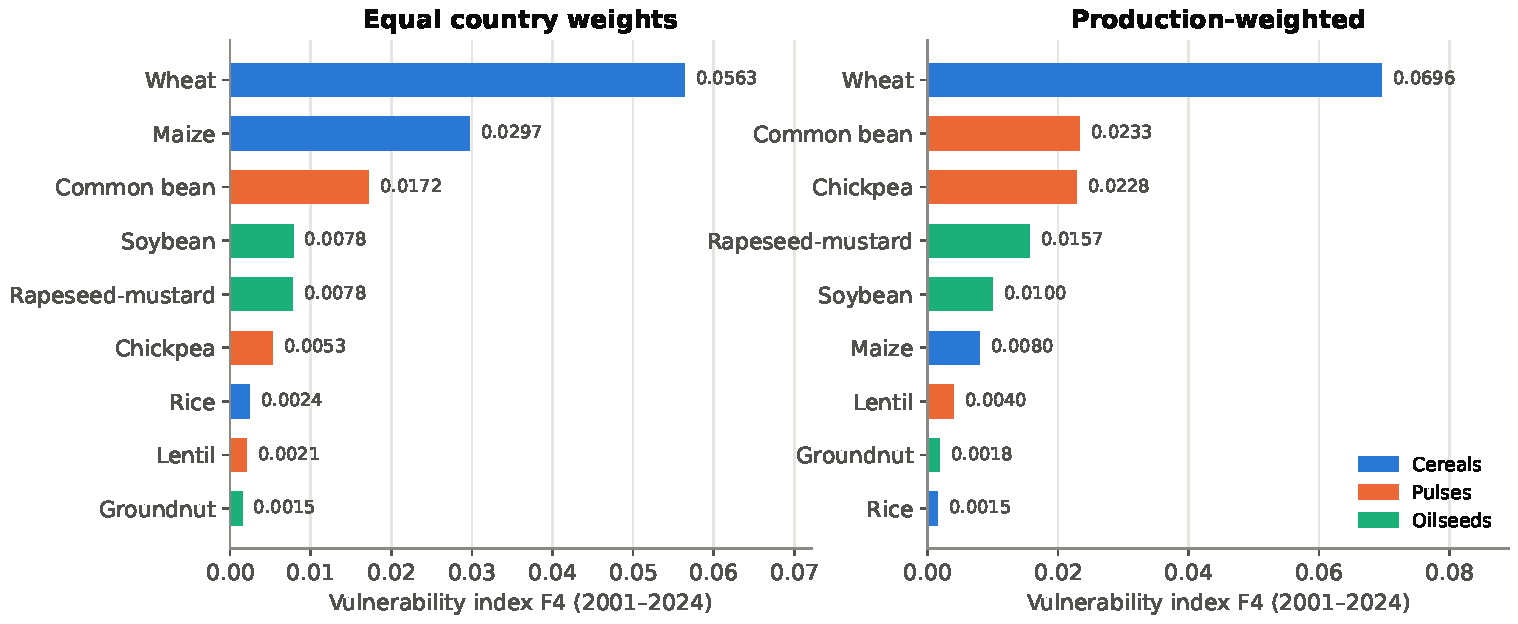
\includegraphics[width=\linewidth]{G01_crop_ranking.pdf}
\caption{Nine-crop vulnerability, 2001--2024 (\Fd). Left: mean over each crop's countries; right: weighted by
each country's production. Colour = crop group.}\label{fig:ranking}
\end{figure}

\paragraph{Order.} With equal country weights the order is \orderEq. Weighted by production it is \orderPw\
(Figure~\ref{fig:ranking}, Table~\ref{tab:cropindex}).

\paragraph{Stability.} Wheat is first under both weightings, in \robTopFfour\ of \robNFfour\ one-at-a-time
robustness rankings of \Fd, and in \mcTopShare\% of 2,000 random weightings (Section~\ref{sec:checks}). Positions
below first are much less stable:
\begin{itemize}
\item \secondEq\ is second with equal weights, but \secondPw\ is second with production weights;
\item rice is near the bottom under both weightings, for reasons explained below.
\end{itemize}

\begin{table}[H]\centering\small
\caption{Crop scores and components, 2001--2024 (equal weights unless marked pw).}\label{tab:cropindex}
\adjustbox{max width=\linewidth}{\begin{tabular}{llrrrrrrrrrr}
\toprule
Crop & Group & n & $E_T$ & $E_P$ & $S_T$ & $S_P$ & $\tilde I$ & F4 eq & rank & F4 pw & rank \\
\midrule
Wheat & Cereals & 6 & 0.03 & 0.23 & 0.50 & 0.88 & 0.53 & 0.0563 & 1 & 0.0696 & 1 \\
Maize & Cereals & 6 & 0.00 & 0.27 & 0.38 & 1.00 & 0.15 & 0.0297 & 2 & 0.0080 & 6 \\
Common bean & Pulses & 7 & 0.39 & 0.29 & 0.56 & 0.92 & 0.07 & 0.0172 & 3 & 0.0233 & 2 \\
Soybean & Oilseeds & 7 & 0.00 & 0.24 & 1.00 & 0.68 & 0.11 & 0.0078 & 4 & 0.0100 & 5 \\
Rapeseed-mustard & Oilseeds & 7 & 0.02 & 0.48 & 0.50 & 0.72 & 0.05 & 0.0078 & 5 & 0.0157 & 4 \\
Chickpea & Pulses & 7 & 0.00 & 0.52 & 0.70 & 0.70 & 0.02 & 0.0053 & 6 & 0.0228 & 3 \\
Rice & Cereals & 7 & 0.00 & 0.05 & 0.35 & 1.00 & 0.28 & 0.0024 & 7 & 0.0015 & 9 \\
Lentil & Pulses & 7 & 0.00 & 0.58 & 0.85 & 0.80 & 0.01 & 0.0021 & 8 & 0.0040 & 7 \\
Groundnut & Oilseeds & 5 & 0.01 & 0.16 & 0.47 & 0.56 & 0.09 & 0.0015 & 9 & 0.0018 & 8 \\
\bottomrule
\end{tabular}
\par\vspace{2pt}{\footnotesize Component columns are equal-weighted means over the crop's panel countries. eq = equal country weights; pw = production-weighted (FAOSTAT 2020--24).}
}
\end{table}

\subsection{What drives the scores}
\begin{figure}[H]\centering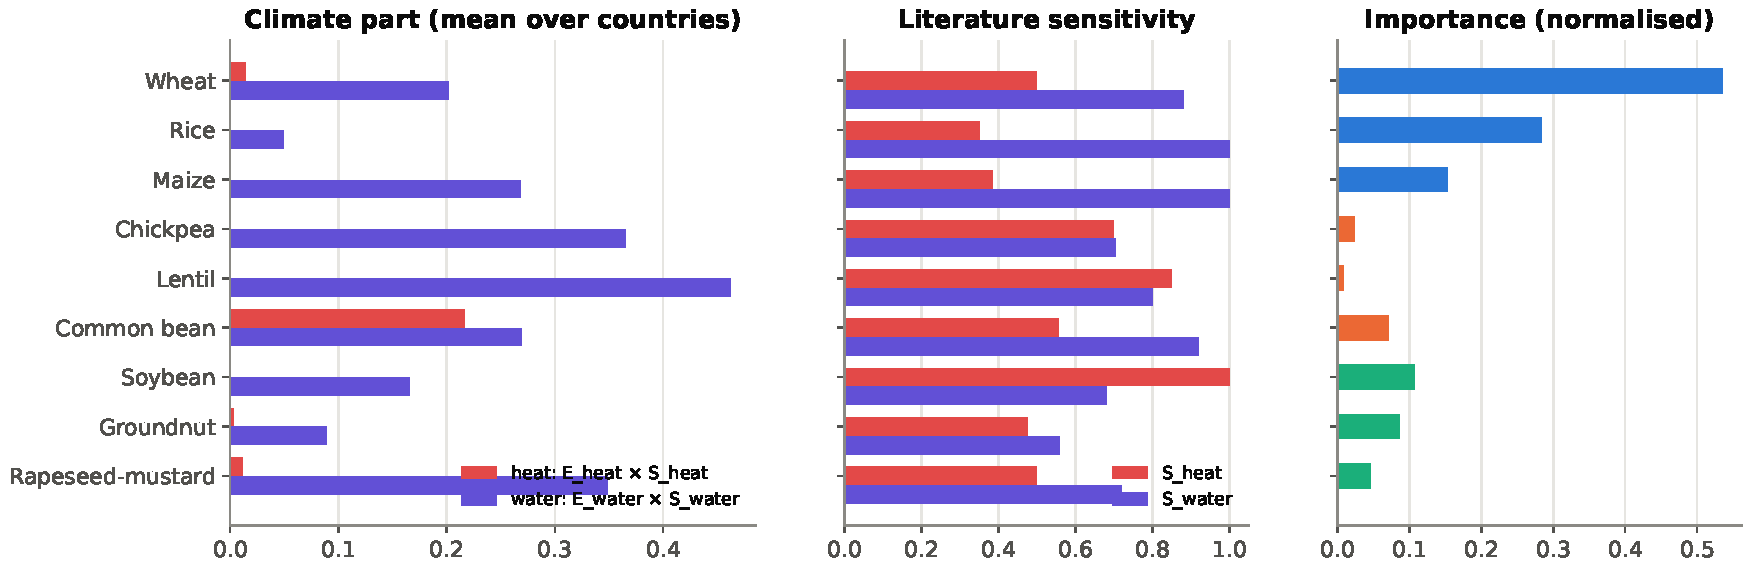
\includegraphics[width=\linewidth]{G03_components.pdf}
\caption{Climate part, sensitivity and importance by crop (equal-weighted means of the pair values).}\label{fig:components}\end{figure}

Figure~\ref{fig:components} separates the three components.
\begin{itemize}
\item \textbf{Wheat} combines high importance with exposure on both hazards. In the 2021--23 food balance sheets it
is the largest single food source of zinc in \wheatTopZinc, of iron in \wheatTopIron\ and of protein in
\wheatTopProtein\ of the \nDivUnits\ units (panel countries and World).
\item \textbf{Maize} is second with equal weights, mainly through two countries.
  \begin{itemize}
  \item South Africa: maize supplies \maizeSAkcal\% of national energy, \maizeSArainfed\% of its area is rainfed,
  and $E_{\text{water}}=\maizeSAEwater$.
  \item Ukraine: the largest water exposure of any maize pair (\maizeUAEwater).
  \end{itemize}
  With production weights maize drops, because in the two largest producers most maize is not eaten: only
  \maizeFoodUSA\% (USA) and \maizeFoodChina\% (China) of domestic supply goes to food.
\item \textbf{Soybean} has the steepest heat slope but zero heat exposure. Its monthly flowering $\Teff$ stays below
\SI{35}{\celsius} in all its countries, and it is eaten mainly as oil.
\item \textbf{Rice} scores low for two reasons, both properties of the measurement rather than proof that rice is
safe:
  \begin{itemize}
  \item most rice is irrigated, which the water measure counts as unstressed;
  \item monthly mean temperatures rarely exceed its \SI{35}{\celsius} anthesis threshold.
  \end{itemize}
\item \textbf{Pulses} enter the top half through common bean (heat) and chickpea (water). Their national importance
is small except in East Africa and South Asia, which keeps lentil low.
\end{itemize}

\subsection{Countries}
\begin{figure}[H]\centering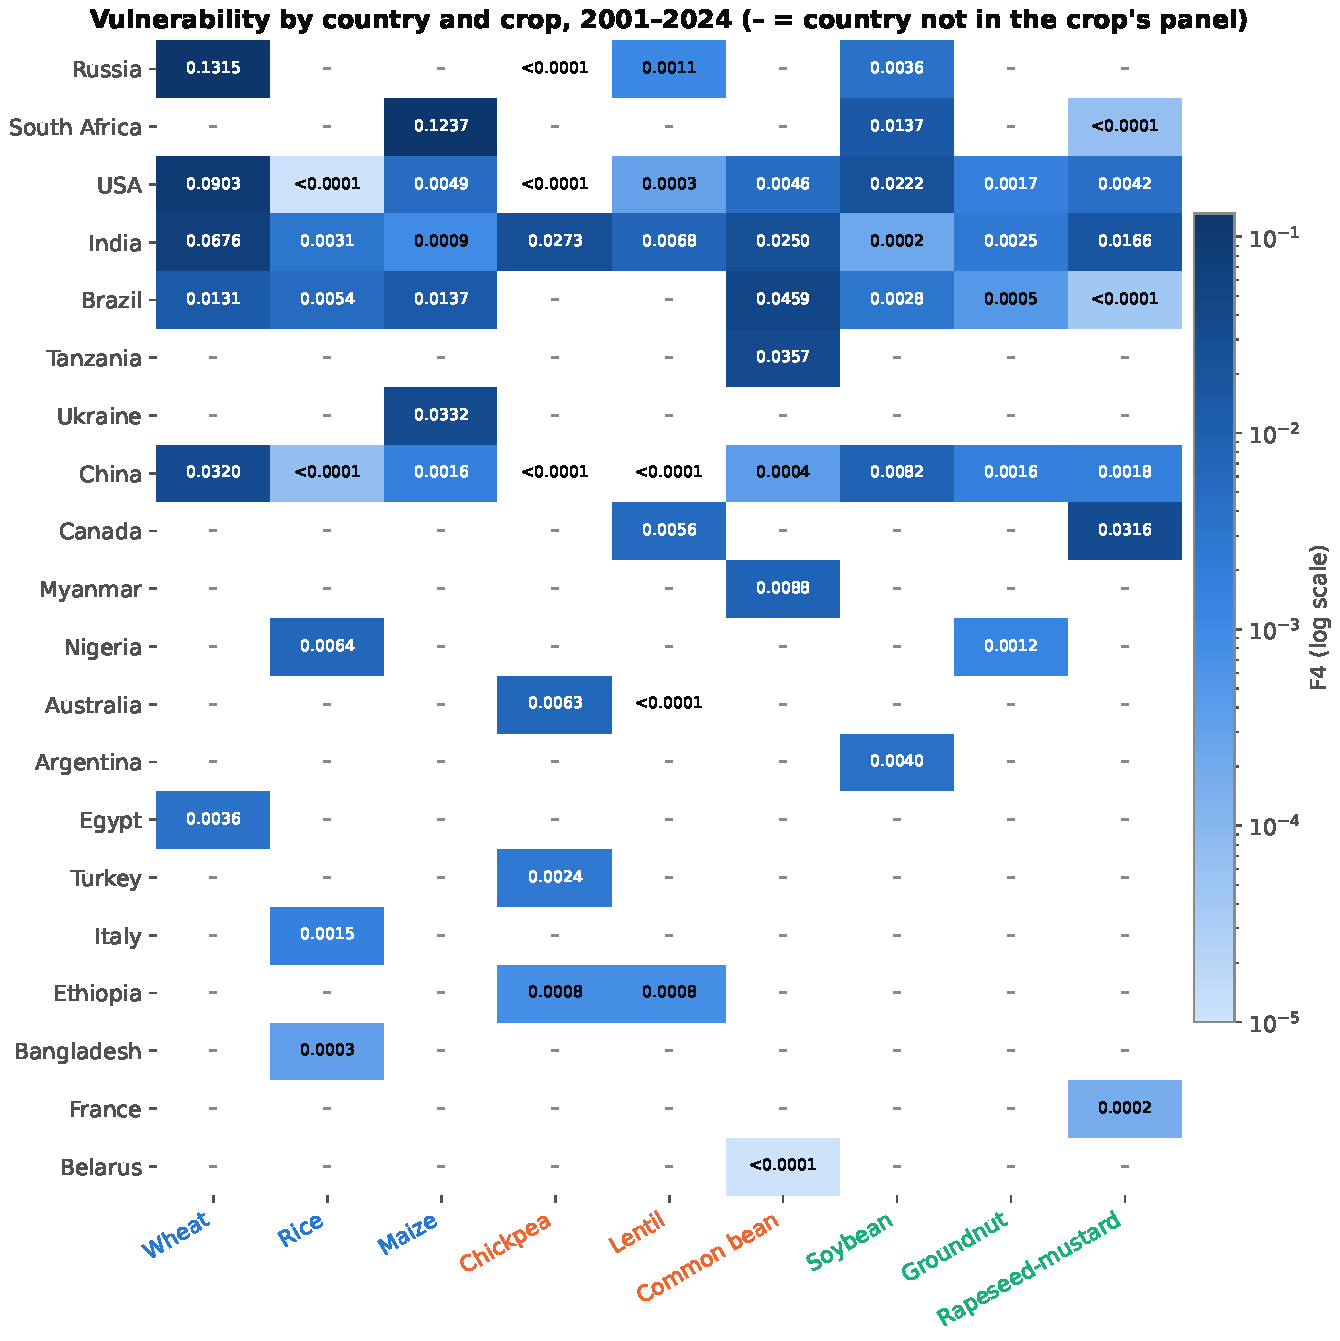
\includegraphics[width=0.92\linewidth]{G02_country_crop_matrix.pdf}
\caption{Country by crop \Fd, 2001--2024 (blank = crop not in that country's panel).}\label{fig:matrix}\end{figure}

\paragraph{Highest pairs.} The highest pairs are \topPairA\ (\topPairAValue), \topPairB\ (\topPairBValue), \topPairC\
(\topPairCValue), \topPairD\ (\topPairDValue), \topPairE\ (\topPairEValue) and \topPairF\ (\topPairFValue)
(Figure~\ref{fig:matrix}). They share one pattern: a crop that is a large part of the national diet \emph{and}
grown on rainfed land where its water need is often unmet. Examples are wheat in the Russian, US and Indian plains,
maize in South Africa, and beans in Brazil and Tanzania.

\paragraph{Water versus heat.} In \nTopSevenWater\ of the seven highest pairs the water term is larger than the heat
term. Over all pairs, water accounts for \presentWaterShare\% of the summed score today. Wheat in India has the
highest wheat heat exposure, but even there the water term is larger once heat is scaled by the panel's highest
heat level. The full country-by-crop table is Table~\ref{tab:countrycrop} (Appendix~\ref{app:tables}).

\subsection{Crop groups}
\begin{figure}[H]\centering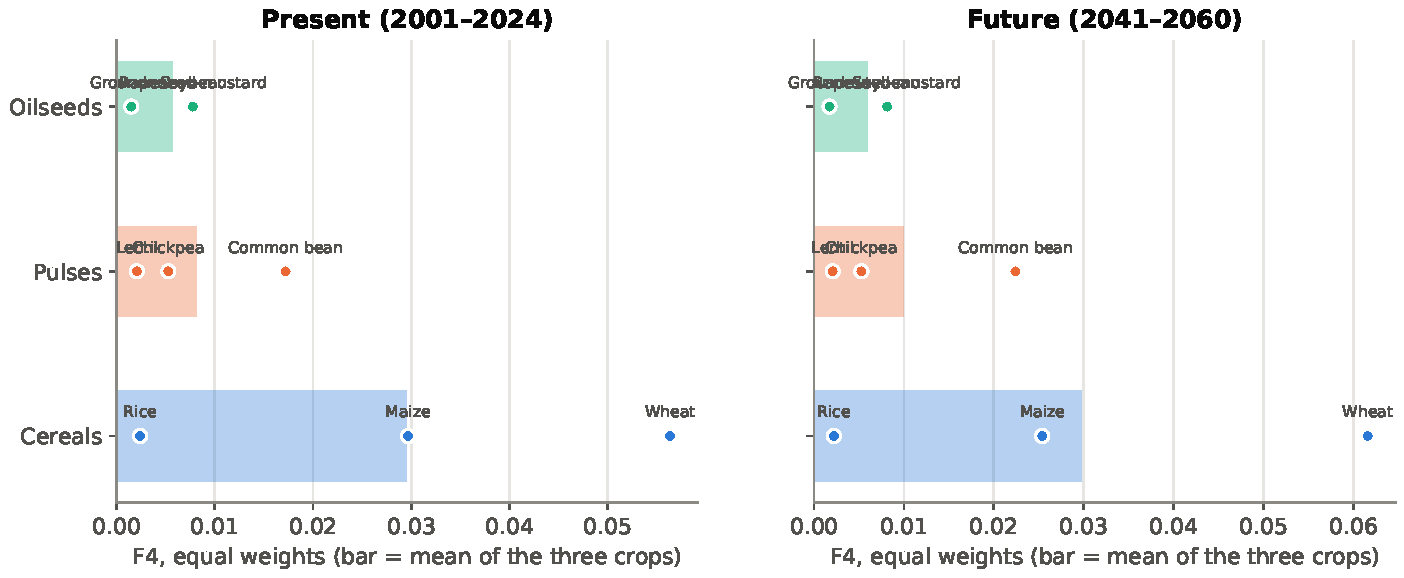
\includegraphics[width=0.85\linewidth]{G06_crop_groups.pdf}
\caption{Crop-group scores (mean of the three selected crops; bars show the range of the crops).}\label{fig:groups}\end{figure}

By group the order is \groupOrder\ (Figure~\ref{fig:groups}, Table~\ref{tab:groups}).
\begin{itemize}
\item The cereal lead comes from wheat and maize.
\item The pulse score comes from common bean and chickpea.
\item The oilseed score is low because soybean and rapeseed are eaten mainly as oil and have little heat
exposure.
\end{itemize}
A group mean describes three selected crops, so it should not be read as a statement about all cereals, pulses
or oilseeds.

\begin{table}[H]\centering\small\caption{Crop-group summaries (equal and production-weighted, with the range over
the three crops).}\label{tab:groups}
\adjustbox{max width=\linewidth}{\begin{minipage}{\textwidth}\centering
\adjustbox{max width=\textwidth}{\begin{tabular}{llrrrrr}
\toprule
Group & Crops & mean F4 eq & crop range & mean F4 pw & 1971--2000 & 2041--2060 \\
\midrule
Cereals & Wheat, Rice, Maize & 0.0295 & 0.0024--0.0563 & 0.0264 & 0.0275 & 0.0297 \\
Pulses & Chickpea, Lentil, Common bean & 0.0082 & 0.0021--0.0172 & 0.0167 & 0.0080 & 0.0099 \\
Oilseeds & Soybean, Groundnut, Rapeseed-mustard & 0.0057 & 0.0015--0.0078 & 0.0092 & 0.0059 & 0.0060 \\
\bottomrule
\end{tabular}
}
\par\vspace{2pt}{\footnotesize Group value = simple mean of the three selected crops; it describes these crops, not every cereal, pulse or oilseed.}
\end{minipage}
}\end{table}

\subsection{How adding crops changed the numbers}
The physical stress of every original pair is unchanged between the four-crop and nine-crop runs, but the
normalisation reference is not.
\begin{itemize}
\item The largest heat level is now \refHeatPair\ (\refHeat\,\si{\celsius} above its threshold), and the largest
water level \refWaterPair\ (\refWater).
\item All original scores therefore roughly halve, while their order is unchanged: \orderOrigFourEq\ in the
four-crop run, \orderOrigNineEq\ within the nine-crop run.
\end{itemize}

The bean reference is itself uncertain. It comes from a chamber-derived threshold for a heat-susceptible Andean
bean, applied to FAO ``beans, dry'', which in India includes tropical \emph{Vigna} pulses. Raising bean's threshold
by \SI{2}{\celsius}, or all new legumes' by \SI{3}{\celsius}, leaves wheat first (Table~\ref{tab:robust}).

Compared with the frozen mid-evaluation numbers, the presented literature-only method gives the same four-crop order
(\orderFourEq), with values higher by a median factor of \litRatioMedian\ (Figure~\ref{fig:midlit},
Appendix~\ref{app:tables}).

\section{Results: how does vulnerability change by 2041--2060?}\label{sec:future}

\begin{figure}[H]
\centering
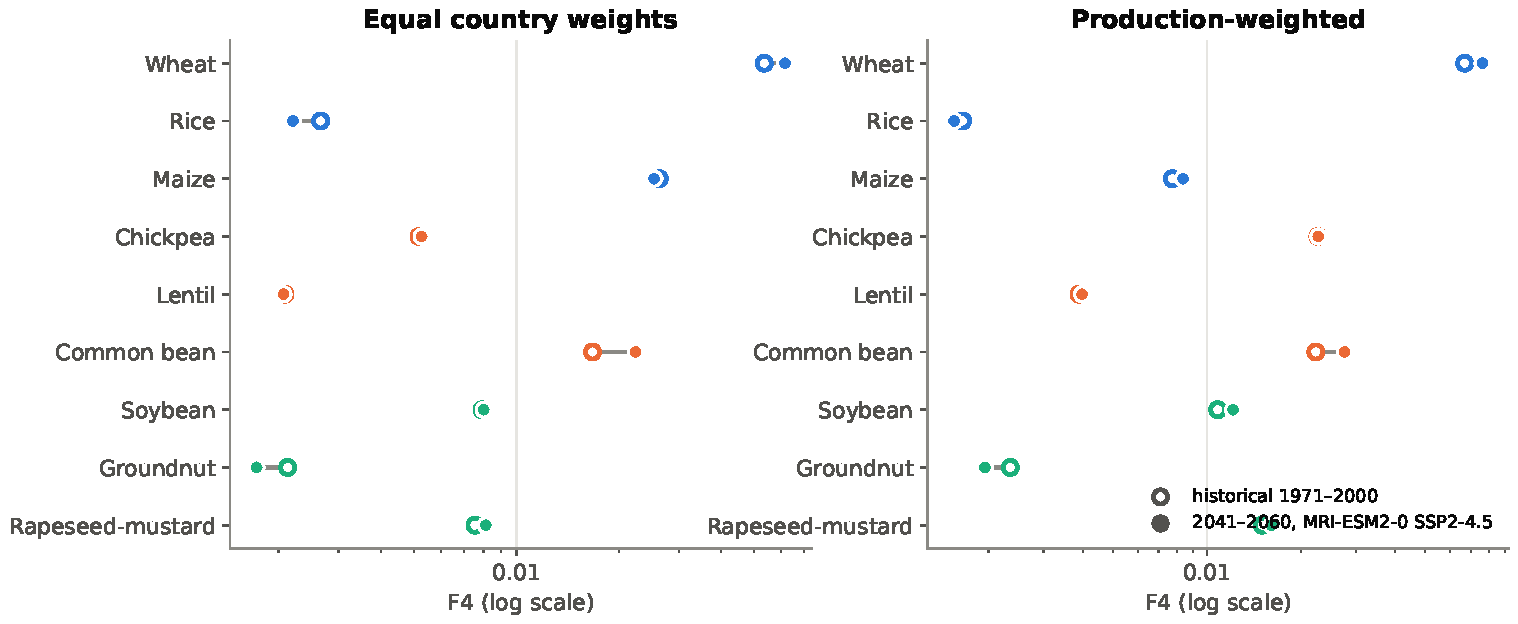
\includegraphics[width=\linewidth]{G04_present_future_crops.pdf}
\caption{Historical (1971--2000, open) and future (2041--2060, filled) crop scores, MRI-ESM2-0 SSP2-4.5, change
factors on the same years, one fixed normalisation reference.}\label{fig:future}
\end{figure}

\subsection{Magnitude and order}
Under one model and one scenario, the flowering-window effective temperature rises by \meanDTeff\,\si{\celsius} on
average over the \nPairs\ pairs.
\begin{itemize}
\item The score rises in \nPairsUp\ of \nPairs\ pairs.
\item \nPairsExceedRef\ pair exceeds the present-day reference maximum (values above one are allowed by
construction).
\item The crop order changes little: \futOrderEq\ with equal weights in 2041--2060, against \histOrderEq\ in
1971--2000 (Figure~\ref{fig:future}, Table~\ref{tab:futurecrop}).
\item Relative to 1971--2000, the equal-weighted group scores change by \grpCerealPct\% (cereals),
\grpPulsePct\% (pulses) and \grpOilseedPct\% (oilseeds). The \grpFastest\ rise fastest, mainly through common bean.
\end{itemize}

\begin{table}[H]\centering\small\caption{Crop scores 2001--24, 1971--2000 and 2041--2060 (fixed normalisation
reference; $\Delta$F4 is a change in index units, not a yield change).}\label{tab:futurecrop}
\adjustbox{max width=\linewidth}{\begin{tabular}{lrrrrrrcrrc}
\toprule
Crop & $\Delta T_{eff}$ & 2001--24 & 1971--2000 & 2041--60 & $\Delta$F4 & \% & rank eq & pairs up & F4 pw 2041--60 & rank pw \\
\midrule
Wheat & +2.0 & 0.0563 & 0.0535 & 0.0616 & +0.0080 & +15\% & 1$\to$1 & 6/6 & 0.0762 & 1$\to$1 \\
Maize & +2.0 & 0.0297 & 0.0263 & 0.0254 & -0.0009 & -3\% & 2$\to$2 & 3/6 & 0.0084 & 6$\to$6 \\
Common bean & +2.0 & 0.0172 & 0.0167 & 0.0224 & +0.0057 & +34\% & 3$\to$3 & 7/7 & 0.0276 & 3$\to$2 \\
Rapeseed-mustard & +2.0 & 0.0078 & 0.0076 & 0.0081 & +0.0006 & +8\% & 5$\to$4 & 7/7 & 0.0161 & 4$\to$4 \\
Soybean & +1.9 & 0.0078 & 0.0079 & 0.0080 & +0.0001 & +1\% & 4$\to$5 & 3/7 & 0.0121 & 5$\to$5 \\
Chickpea & +2.0 & 0.0053 & 0.0052 & 0.0053 & +0.0001 & +2\% & 6$\to$6 & 3/7 & 0.0227 & 2$\to$3 \\
Rice & +1.8 & 0.0024 & 0.0027 & 0.0022 & -0.0005 & -17\% & 7$\to$7 & 5/7 & 0.0016 & 9$\to$9 \\
Lentil & +2.2 & 0.0021 & 0.0021 & 0.0021 & -0.0000 & -1\% & 9$\to$8 & 4/7 & 0.0040 & 7$\to$7 \\
Groundnut & +1.6 & 0.0015 & 0.0021 & 0.0017 & -0.0004 & -19\% & 8$\to$9 & 2/5 & 0.0019 & 8$\to$8 \\
\bottomrule
\end{tabular}
\par\vspace{2pt}{\footnotesize MRI-ESM2-0, SSP2-4.5, change factors on 1971--2000 years; one fixed normalisation reference (2001--24 nine-crop maxima); sensitivity, importance, crop area, irrigation and calendars held fixed. $\Delta T_{eff}$ = mean change in flowering-window effective temperature (\si{\celsius}). \% only where the historical score is $\geq$1\% of the largest.}
}\end{table}

\subsection{Heat and water parts of the change}
The change splits exactly into heat and water parts (Eq.~\ref{eq:decomp}).
\begin{itemize}
\item Summed over all pairs, the heat term contributes about \futHeatShare\% of the increase and the water term
\futWaterShare\%. The future increase is mainly heat, while today's scores are mainly water.
\item The largest increase is \futTopPair\ (\futTopPairChange), about two-thirds of it through water. Wheat in
India and common bean in India, Brazil and Myanmar rise almost entirely through heat. Wheat in the USA and bean in
Tanzania rise through heat and water in similar measure (Figure~\ref{fig:futurepairs},
Table~\ref{tab:futurepairs}; pair values in \file{future\_components.csv}).
\item Every pair whose score falls does so through the water term alone. In those pairs the change factors give a
smaller rainfed deficit, while the heat term stays near zero. Examples are rice, maize, soybean and groundnut in
some countries, such as maize in South Africa and rice in Nigeria.
\end{itemize}

\begin{figure}[H]\centering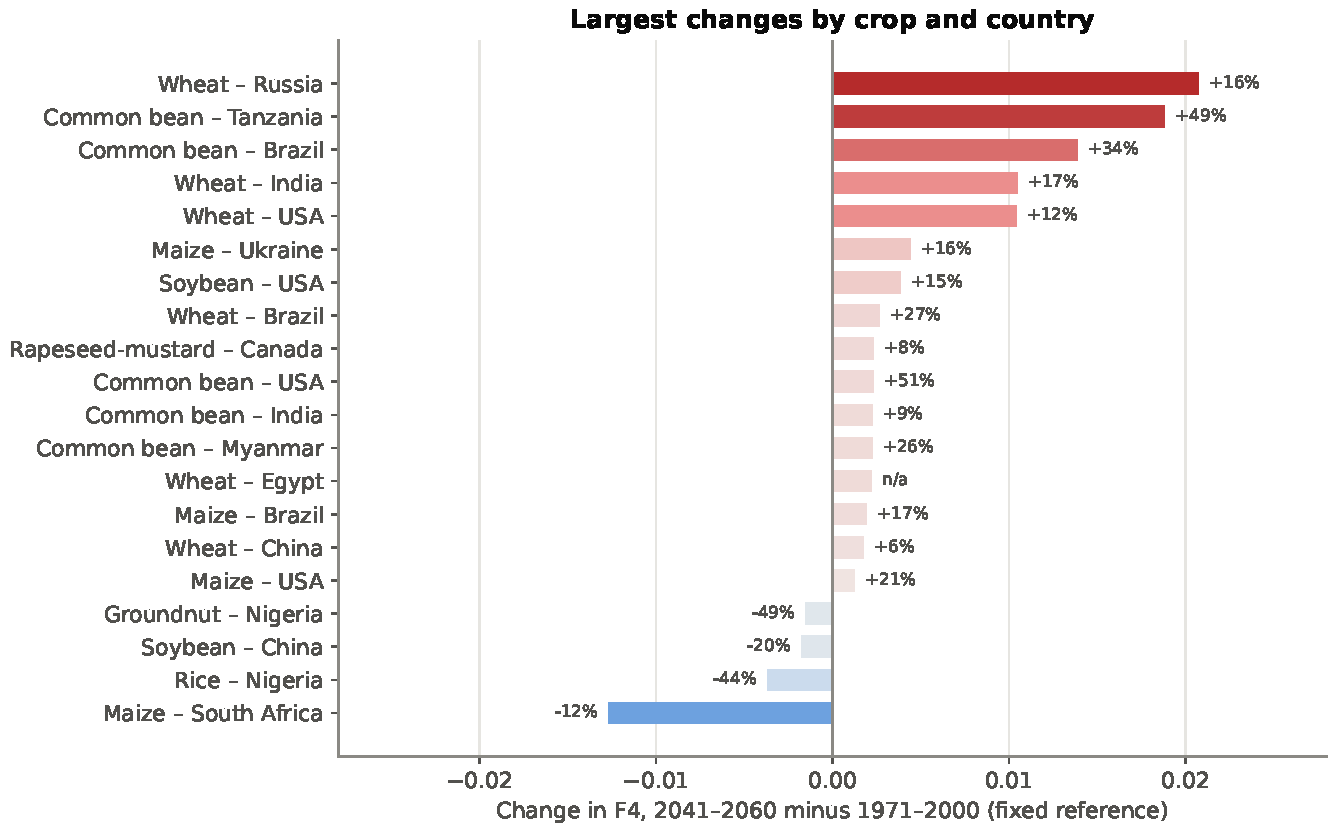
\includegraphics[width=0.85\linewidth]{G05_future_pairs.pdf}
\caption{Largest changes in pair scores, split into heat and water parts.}\label{fig:futurepairs}\end{figure}

\subsection{Does the result depend on the method?}
The climatology check applies the thresholds directly to the 20-year means instead of using change factors. It
gives the same sign of change in \climCheckSameSign\% of pairs, with Spearman $\rho$ = \climCheckRho\ between the
two sets of changes. The direction of change therefore does not hinge on the change-factor choice. It does depend
on the single climate model: the wetter South African maize season, for example, is a property of MRI-ESM2-0, and
other models disagree on regional rainfall.

\subsection{Interpretation}
A crop can stay nutritionally important while its climate stress rises, and a low score can still reflect the
monthly heat measure. The future index values are scores relative to today's maxima, not yield losses. The yield
and nutrient consequences are estimated separately in Section~\ref{sec:futurenut}.

\section{Results: what does a crop loss mean for nutrient supply?}\label{sec:nutrition}

\subsection{What each crop supplies}
\begin{figure}[H]\centering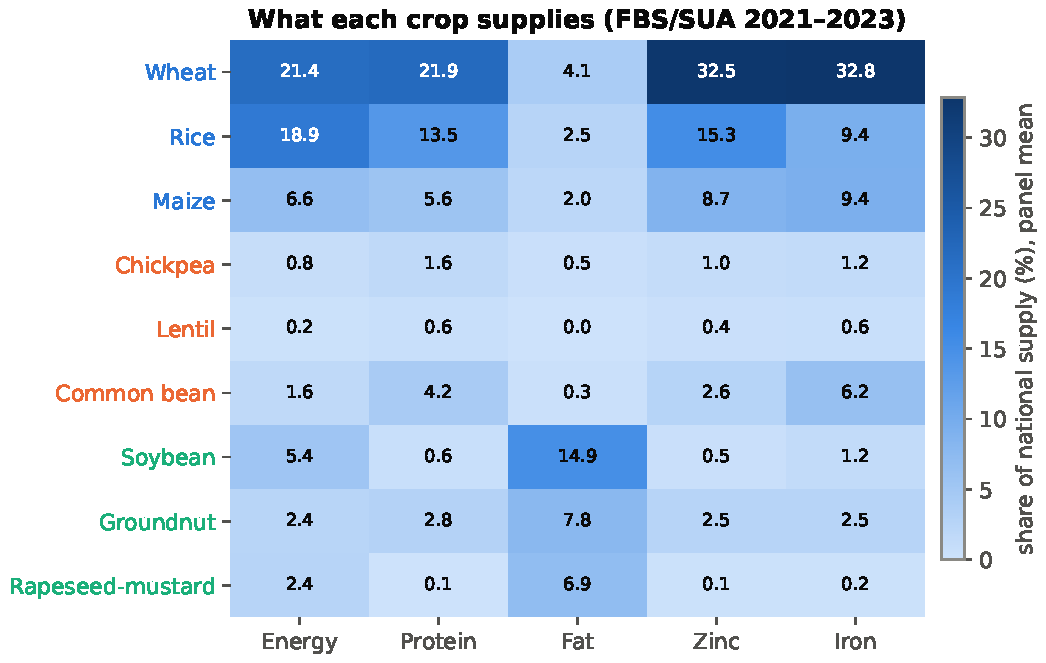
\includegraphics[width=0.8\linewidth]{G07_nutrient_profiles.pdf}
\caption{Share of national supply of each nutrient from each crop (mean over the crop's panel countries, FBS 2021--23).}\label{fig:profiles}\end{figure}
\begin{itemize}
\item \textbf{Cereals} dominate energy, protein, zinc and iron.
\item \textbf{Oilseeds} mainly supply fat, as oil. Soybean is mostly crushed, so the FBS credit it with almost no
food protein.
\item \textbf{Pulses} matter for protein and iron, mostly in South Asia and East Africa (Figure~\ref{fig:profiles}).
\end{itemize}

\subsection{Adequacy}
Iron is the nutrient most often below requirement: \nIronShort\ of \nAdqCountries\ panel countries under the main
requirement. Energy, protein, fat and zinc are below requirement in none (Table~\ref{tab:adequacy}). The iron
result depends on the requirement chosen: with iron at 15\% bioavailability, \nIronShortAlt\ countries fall short.
Section~\ref{sec:adequacy} explains why national ratios are a supply-side screen.

\subsection{A standard 10\% yield loss}
\begin{figure}[H]\centering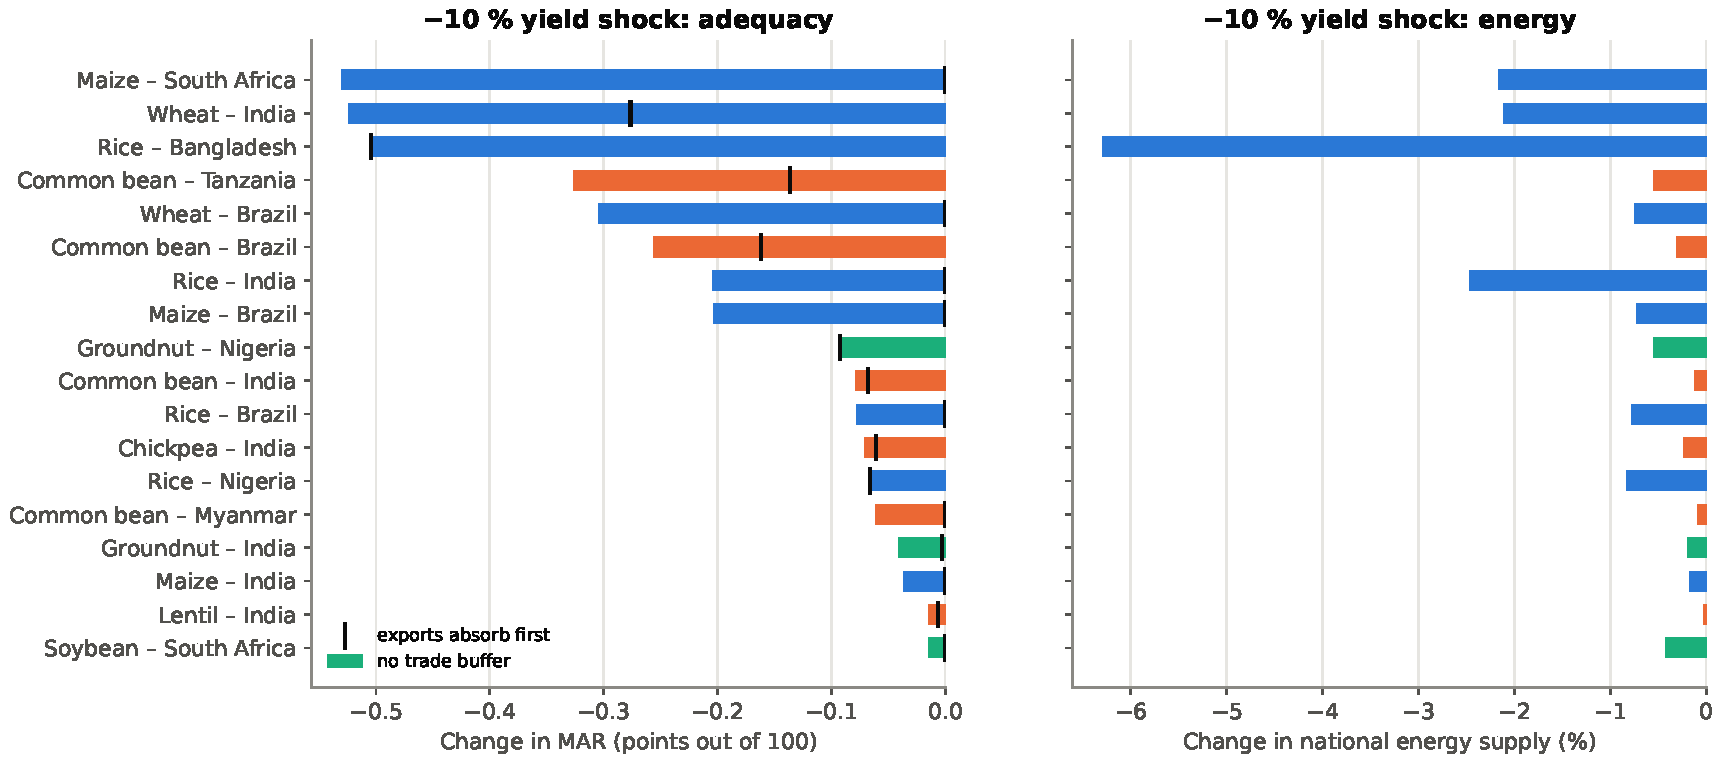
\includegraphics[width=0.95\linewidth]{G08_yield_shock.pdf}
\caption{Standard $-10\%$ yield loss: change in national energy supply and in MAR for the pairs with the largest
MAR change (upper bound and export-buffered lower bound).}\label{fig:shock}\end{figure}

\paragraph{MAR.} Removing 10\% of a crop's production share of supply changes national MAR by less than 0.005
points in \shockZeroMar\ of \shockN\ pairs. This is because national supply stays above requirement for most
nutrients.
\begin{itemize}
\item The largest MAR fall is \shockTopMar\ (\shockTopMarValue\ points).
\item The largest energy loss is \shockTopKcal\ (\shockTopKcalValue\% of national kcal).
\end{itemize}
Because MAR caps each ratio at one, it hides losses that still leave supply above requirement, so the nutrient
losses themselves are reported alongside (Figure~\ref{fig:shock}, Table~\ref{tab:shock}). The largest MAR changes
come where iron is already short and the shocked crop is an iron source.

\paragraph{History.} In the old food balance sheets (1961--2013), a bad harvest significantly lowered food supply
in \passOldPos\ of \passOldN\ pairs; in the new series (2010--2023), in \passNewPos\ of \passNewN.
\begin{itemize}
\item These are associations. Trade and stocks buffer most losses.
\item The new series has only 14 years, so an insignificant estimate there is not proof of buffering.
\end{itemize}

\subsection{Conditional future yield and nutrient change}\label{sec:futurenut}
\begin{figure}[H]\centering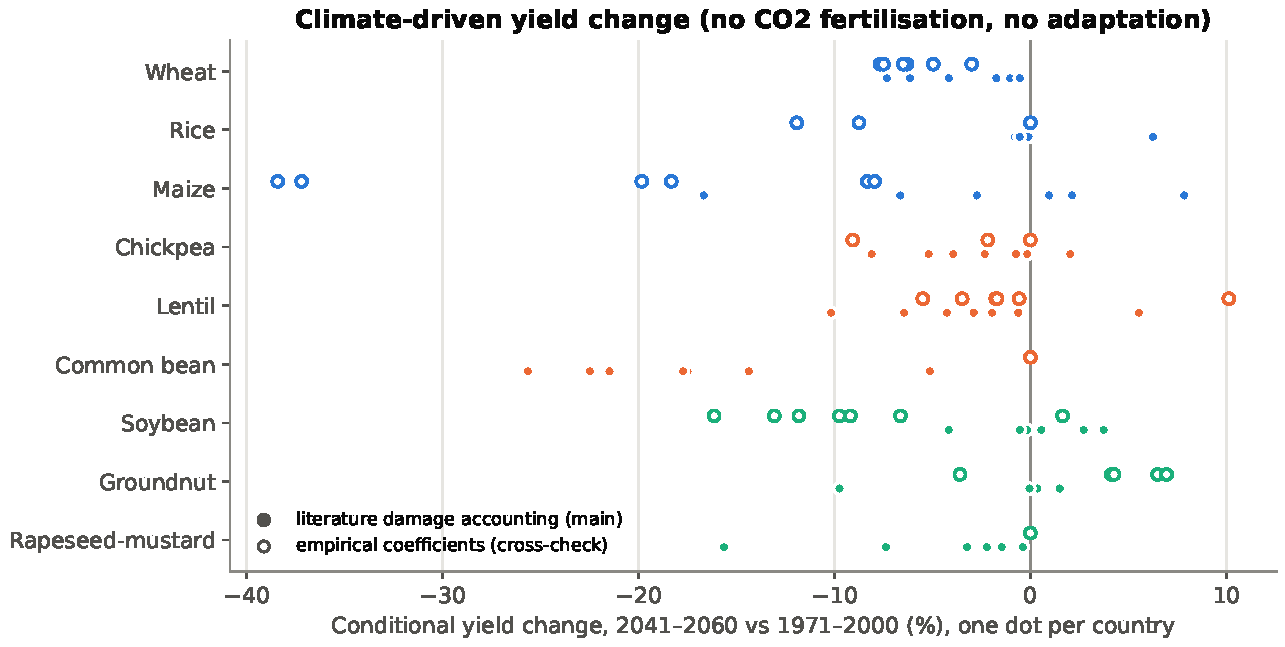
\includegraphics[width=0.9\linewidth]{G09_future_yield.pdf}
\caption{Climate-driven yield change 1971--2000 $\to$ 2041--2060 by crop: literature damage accounting (main)
and empirical coefficients (cross-check).}\label{fig:futyield}\end{figure}

\paragraph{Main estimate.} The literature damage accounting (Section~\ref{sec:futureyield}) gives a yield loss in
\fyLitNeg\ of \fyN\ pairs.
\begin{itemize}
\item The largest mean loss by crop is for \futYieldWorst\ (\futYieldWorstValue\%), driven by heat during
flowering.
\item The largest nutrient consequence is \futNutTopPair\ (MAR \futNutTopMar\ points)
(Table~\ref{tab:futyield}, Table~\ref{tab:futnut}).
\end{itemize}

\paragraph{Empirical cross-check.} The empirical coefficients give a loss in \fyEmpNeg\ of \fyN\ pairs and
detect any climate response in \fyEmpDetected\ of \fyN.
\begin{itemize}
\item The two methods agree in sign for \fySameSign\% of pairs.
\item Their pair-level rank correlation is \corrLitEmp.
\end{itemize}

\paragraph{Why they differ.}
\begin{itemize}
\item The literature functions describe yield damage above a threshold under controlled conditions.
\item The regressions describe how national yields co-varied with monthly climate in 1971--2000, including
adaptation and irrigation, with few statistically clear heat effects.
\item Common bean has the largest literature loss but no detectable empirical climate response in any of its
countries.
\item Maize shows the opposite contrast. Its empirical coefficients imply much larger losses than the literature
accounting. Its fitted heat coefficients are steep (the US and South African country estimates and the pooled
panel estimate used elsewhere), while maize's literature threshold of \SI{32}{\celsius} on monthly $\Teff$ is
rarely crossed.
\end{itemize}
Neither method is validated against future yields. Their disagreement is the main uncertainty in the future
nutrient numbers.

\paragraph{Status.} The future nutrient numbers are therefore reported as a \textbf{conditional screening
estimate}: what the literature damage functions imply under one climate model with today's crop area and diets.
They are not a forecast, and they are not confirmed by the observed yield record.

\begin{table}[H]\centering\small\caption{Conditional climate-driven yield change by crop, 1971--2000 $\to$
2041--2060 (literature accounting and empirical cross-check).}\label{tab:futyield}
\adjustbox{max width=\linewidth}{\begin{tabular}{lrrrr}
\toprule
Crop & $\Delta T_{eff}$ \si{\celsius} & $\Delta Y$ lit (mean \%) & range over countries & $\Delta Y$ empirical (mean \%) \\
\midrule
Wheat & +2.0 & -3.5 & -7.3 to -0.5 & -6.0 \\
Rice & +1.8 & +0.7 & -0.8 to +6.3 & -3.0 \\
Maize & +2.0 & -2.5 & -16.7 to +7.8 & -21.7 \\
Chickpea & +2.0 & -2.6 & -8.1 to +2.0 & -1.6 \\
Lentil & +2.2 & -3.0 & -10.2 to +5.5 & -0.7 \\
Common bean & +2.0 & -17.8 & -25.6 to -5.1 & +0.0 \\
Soybean & +1.9 & +0.7 & -4.2 to +3.7 & -9.3 \\
Groundnut & +1.6 & -1.3 & -9.7 to +1.5 & +3.6 \\
Rapeseed-mustard & +2.0 & -5.4 & -15.6 to -0.4 & +0.0 \\
\bottomrule
\end{tabular}
}\end{table}

% India, Telangana and Hyderabad: what the index says locally. All numbers come from generated macros
% (numbers_india.tex) computed from FAOSTAT, WorldClim/CMIP6, SPAM and official surveys listed in
% docs/evidence/india_hyderabad_sources.md (MoSPI HCES 2023-24 and NSS 594, NFHS-5, CNNS, ICMR-NIN IFCT 2017, Telangana DES).
\section{What the index says for India and for Hyderabad}\label{sec:india}

\subsection{India}
India is in the panel for all nine crops, so the whole ranking can be read for one country: \indOrder.
Wheat (\indWheatFFour) is first; chickpea (\indChickpeaFFour) and common bean (\indBeanFFour) follow. The heat
and water parts differ by crop: wheat's score is mostly water today but its projected increase to 2041--2060
is almost all heat (change in \Fd\ \indWheatdFFour, flowering $\Teff$ \indWheatdTeff\,\si{\celsius}); chickpea's
is entirely water (the rainfed deficit is the highest in the panel, which is why chickpea sets the water
reference); common bean's is mostly heat (about three-fifths) with the rest water. Wheat supplies \indWheatShKcal\% of
India's energy, \indWheatShProtein\% of protein and \indWheatShIron\% of iron, so the stress on wheat is a
stress on iron. A standard 10\% loss of the wheat crop changes national energy supply by \indWheatShockKcal\% and national
iron supply by \indWheatShockIron\%, and MAR by \indWheatShockMar\ points (out of 100), the largest change of
any Indian crop. Under climate change alone (literature accounting, no CO$_2$ fertilisation or adaptation) wheat
yield changes by \indWheatdY\% in 2041--2060 and lentil by \indLentildY\%.

India's food supply is concentrated: the effective number of food items supplying its energy is \divIndKcal\
(Shannon diversity of the FAO food-balance supply, 2021--23, following \citealp{remans2014}), against \divWorldKcal\ for the world, \divUsaKcal\
for the United States and \divChnKcal\ for China; cereals provide \divIndCereal\% of energy; and wheat is the
largest single source of iron (\divIndIronTopShare\%). The nine index crops together supply \divIndNineKcal\% of India's energy,
\divIndNineProtein\% of its protein and \divIndNineIron\% of its iron (national totals from the food balance sheets; chickpea
and lentil from FAOSTAT supply-utilization accounts, because the food balance sheets only report them inside ``Pulses, other'').
Table~\ref{tab:indiashares} shows the shares to two decimals and the correction made in this audit: an earlier version
counted only the seven crops with an FBS item of their own and so left out chickpea and lentil
(Appendix~\ref{app:corrections}).

\begin{table}[H]\centering\small
\caption{Share of India's national supply from the study crops, 2021--23 (numerator: summed crop contributions;
denominator: FBS national total).}\label{tab:indiashares}
\begin{tabular}{lrrr}
\toprule
Nutrient & seven FBS-item crops (\%) & + chickpea, lentil (SUA, \%) & nine crops (\%) \\
\midrule
Energy & 55.19 & 2.81 & 58.00 \\
Protein & 48.94 & 6.36 & 55.30 \\
Fat & 34.12 & 1.59 & 35.71 \\
Zinc & 60.23 & 4.25 & 64.48 \\
Iron & 50.56 & 5.26 & 55.82 \\
\bottomrule
\end{tabular}

\end{table}

\subsection{Hyderabad: what is known, and at what resolution}
Official data are not published for Hyderabad at every level. Household food consumption (MoSPI HCES 2023--24)
and nutrient intake (NSS report 594) are published by state and by rural/urban sector, so
\emph{Telangana urban} is used as the nearest official description of Hyderabad's diet (Hyderabad is the
state's dominant city, but the figures are not city-specific). The National Family Health Survey (NFHS-5,
2019--21) publishes a \emph{Hyderabad district} fact sheet, which is fully urban. Climate is computed for the
WorldClim grid cell containing Hyderabad (\SI{17.4}{\degree}N, \SI{78.5}{\degree}E; 10 arc-minute, roughly
\SI{18}{km}), and crop exposure for all of Telangana (Natural Earth boundary).

Table~\ref{tab:datalevels} keeps these levels apart. In particular:
\begin{itemize}
\item no statement below is a measurement of Hyderabad \emph{city} diets;
\item ``Hyderabad district'' refers only to the NFHS-5 health and nutrition indicators;
\item ``urban Telangana'' refers to household acquisition and intake estimates.
\end{itemize}

\begin{table}[H]\centering\small
\caption{Levels of data used in this section and what each can and cannot say.}\label{tab:datalevels}
\begin{tabular}{p{3.0cm}p{3.6cm}p{3.6cm}p{4.4cm}}
\toprule
Level & Source & Measures & Cannot say \\
\midrule
National supply & FAOSTAT FBS/SUA 2021--23 & food available per person (supply) & who eats it; household or individual intake \\
State $\times$ sector households & MoSPI HCES 2023--24; NSS 594 & quantities acquired and estimated intake, urban Telangana & Hyderabad city specifically; individual diets \\
District measurements & NFHS-5 Hyderabad district fact sheet (2019--21) & anaemia, BMI, child growth (fully urban district) & diet composition \\
State micronutrient status & CNNS 2016--18 Telangana & ferritin, zinc in children and adolescents & district or city values \\
Grid cell / state area & WorldClim; SPAM; Telangana DES & local climate; Telangana crop area and exposure & where Hyderabad's food is grown \\
\bottomrule
\end{tabular}
\end{table}

\subsection{How diverse is the diet?}
\paragraph{Staples.} A person in urban Telangana acquires \hqTgUrbanKgRice\,kg of rice and
\hqTgUrbanKgWheat\,kg of wheat or atta per month: rice is \hqTgUrbanRiceToWheat\ times wheat, against
\hqInUrbanRiceToWheat\ for urban India as a whole (\hqInUrbanKgRice\,kg rice, \hqInUrbanKgWheat\,kg wheat). Cereals
provide \hqKcalCerealTgUrban\% of energy (urban India \hqKcalCerealInUrban\%) and \hqProtCerealTgUrban\% of protein
(\hqProtCerealInUrban\%). Hyderabad's staple is therefore rice, not wheat, which sets it apart from the national
picture above.

\paragraph{Protein sources.} Average intake in urban Telangana is \hqIntakeKcalTgUrban\,kcal,
\hqIntakeProtTgUrban\,g protein and \hqIntakeFatTgUrban\,g fat per person per day (all-India urban:
\hqIntakeKcalInUrban, \hqIntakeProtInUrban, \hqIntakeFatInUrban). Protein comes from cereals
(\hqProtCerealTgUrban\%), pulses (\hqProtPulseTgUrban\%), milk (\hqProtMilkTgUrban\%), eggs, fish and meat
(\hqProtAnimalTgUrban\%, against \hqProtAnimalInUrban\% in urban India) and other foods. The effective number of
protein sources (Shannon diversity over MoSPI's five groups) is \hqProtEffTgUrban\ in urban Telangana and
\hqProtEffInUrban\ in urban India: in this coarse measure Hyderabad's protein diversity is the same as the
national urban average. The animal-source share is higher.

\paragraph{Food groups (NFHS-5, women 15--49, Telangana).} At least weekly: pulses \hqWeeklyPulses\%, milk or curd
\hqWeeklyMilk\%, eggs \hqWeeklyEgg\%, chicken or meat \hqWeeklyMeat\%, dark green leafy vegetables
\hqWeeklyLeafy\%, fruit \hqWeeklyFruit\%, fish \hqWeeklyFish\%. Daily: milk \hqDailyMilk\%, pulses \hqDailyPulses\%,
leafy vegetables \hqDailyLeafy\%, fruit \hqDailyFruit\%, fish \hqDailyFish\%. The gaps are fruit, leafy
vegetables and fish, which are the usual sources of vitamin C, folate and bioavailable iron.

\paragraph{Pulses and where they come from.} Listed pulses amount to \hqTgUrbanKgPulses\,kg per person per
month (urban India \hqInUrbanKgPulses); tur (pigeon pea, not one of our nine crops) is \hqTgUrbanShareTur\% of it,
moong \hqTgUrbanShareMoong\%, gram (chickpea) \hqTgUrbanShareChick\% and masur (lentil) \hqTgUrbanShareLentil\%.
Only the chickpea and lentil shares are covered by the index.

\subsection{Nutrient diversity: where does Hyderabad's iron come from?}
The HCES quantities of the listed grains and pulses, multiplied by the iron and zinc content of the matching
foods in the Indian Food Composition Tables (ICMR-NIN 2017), give the following sources of iron in urban Telangana
(urban India in brackets): rice \hqTgUrbanFeRice\% (\hqInUrbanFeRice\%), wheat \hqTgUrbanFeWheat\%
(\hqInUrbanFeWheat\%), chickpea \hqTgUrbanFeChickpea\% (\hqInUrbanFeChickpea\%), lentil \hqTgUrbanFeLentil\%
(\hqInUrbanFeLentil\%), tur \hqTgUrbanFeTur\%, moong \hqTgUrbanFeMoong\%, groundnut \hqTgUrbanFeGroundnut\%, other
cereals \hqTgUrbanFeOtherCereal\%. The crops of this study supply \hqTgUrbanFeStudy\% of the iron in these foods.
The comparison with India is the point: nationally wheat provides most of the iron from these foods, whereas in
Hyderabad rice does, and rice is a poor iron source (\SI{0.65}{mg} per \SI{100}{g}, against 6.1--7.1 for
chickpea and lentil dal). The listed foods yield \hqTgUrbanFeListed\,mg of iron and \hqTgUrbanZnListed\,mg of zinc
per person per day (urban India: \hqInUrbanFeListed\ and \hqInUrbanZnListed); these are lower bounds, because
vegetables, meat, fish and milk are not included, and they are quantities acquired by households, not intake.

\paragraph{Does the nutrition data show it?} In the Hyderabad district, \hydAnaemChild\% of children 6--59 months
and \hydAnaemNPW\% of non-pregnant women are anaemic (Telangana: \tgAnaemChild\% and \tgAnaemNPW\%; India,
women: \inAnaemNPW\%), while only \hydBmiLow\% of women are underweight and \hydOverweight\% are overweight or obese
(Telangana: \tgBmiLow\% and \tgOverweight\%; India: \inOverweight\% overweight or obese). Energy is not the
problem; iron is. This matches the index's finding that iron is the nutrient closest to shortfall, and it shows
that for a rice-based urban diet the shortfall is one of nutrient density, not quantity. For Telangana,
the national nutrition survey (CNNS 2016--18) found low serum ferritin in \cnnsIronCFour\% of children 1--4 years,
\cnnsIronCNine\% of children 5--9 and \cnnsIronAdol\% of adolescents, and zinc deficiency in \cnnsZincCFour\%,
\cnnsZincCNine\% and \cnnsZincAdol\%.

\subsection{How would climate affect Hyderabad's diet?}
\paragraph{Local climate (grid cell).} Mean daily maximum temperature rose from \hydTmaxBase\ to
\hydTmaxRecent\,\si{\celsius} between 1971--2000 and 2001--2024 (trend \hydTmaxTrend\,\si{\celsius} per decade;
minimum temperature \hydTminTrend), while annual rainfall rose from \hydRainBase\ to \hydRainRecent\,mm. April--May
maximum temperature, the hottest season, changed little (\hydAMBase\ to \hydAMRecent\,\si{\celsius}). Under
MRI-ESM2-0 SSP2-4.5, 2041--2060 minus the 1970--2000 normal: April--May maximum $+$\hydAMFutChange\,\si{\celsius}
(to \hydAMFutLevel\,\si{\celsius}), mean minimum $+$\hydTminFutChange\,\si{\celsius}, annual rainfall \hydRainFutRatio\%.
One model, one scenario.

\paragraph{Factor 1 --- heat on Telangana's crops.} Rice is the dominant crop (\tgAreaRice\% of Telangana
cropland in the 2010 SPAM map, then cotton \tgAreaCotton\%, maize \tgAreaMaize\%, common bean \tgAreaBean\%).
Heat exposure of rice and maize is essentially zero (monthly flowering temperature is below the rice
\SI{35}{\celsius} and maize \SI{32}{\celsius} thresholds), whereas the common bean area (\tgBeanEheatTwoZeroZeroOneTwoZeroTwoFour\ times the panel reference maximum)
is above its threshold. Flowering temperature in Telangana rises by \tgRicedTefffutureC\,\si{\celsius} for
rice by 2041--2060 (wheat, with a very small area: \tgWheatdTefffutureC).

\paragraph{Factor 2 --- water.} Telangana rice is \tgRiceRainfed\% rainfed, i.e.\ \emph{almost entirely
irrigated}, so the index gives it almost no water stress today, and by 2041--2060 the model projects a smaller
deficit. This is the weak point of the result: the index treats irrigation as a guaranteed buffer. Telangana's
own statistics put paddy at \tgPaddyAreaMha\,Mha in 2023--24 against \tgPaddySpamMha\,Mha in the 2010 map
(\tgPaddyGrowth\ times larger), so the area on which this buffer depends has grown a great deal; the index
cannot say whether that irrigation can be sustained. The other crops that matter for iron are rainfed:
chickpea (\tgChickpeaRainfed\% rainfed), maize (\tgMaizeRainfed\%) and groundnut (\tgGroundnutRainfed\%); chickpea's
water exposure in Telangana is \tgChickpeaEwaterTwoZeroZeroOneTwoZeroTwoFour\ times the panel reference maximum.

\paragraph{What this means for iron intake.} Taking the crops that supply Hyderabad's iron and the climate-driven
yield change under the literature accounting (Telangana climate for rice, maize, chickpea and groundnut; the
national figure for wheat, since Telangana grows almost no wheat, and for lentil): rice \hqdYRice\%, maize
\hqdYMaize\%, chickpea \hqdYChickpea\%, groundnut \hqdYGroundnut\%, wheat \hqdYWheat\%, lentil \hqdYLentil\%. Weighted
by their shares of listed iron, the change in iron from these foods is \hqIronChangeUrban\% for urban Telangana.
A standard 10\% loss of a single crop would lower the iron from these foods by \hqIronTenRiceUrban\% (rice),
\hqIronTenWheatUrban\% (wheat) or \hqIronTenChickpeaUrban\% (chickpea). These are accounting estimates with no market
response, no CO$_2$ fertilisation and no adaptation, not forecasts.

\subsection{What the index indicates for Hyderabad}
\begin{enumerate}
\item \textbf{Hyderabad's diet is less exposed to the crop that dominates the national ranking.} Wheat is the
most vulnerable crop in India, but it supplies about a fifth (\hqTgUrbanFeWheat\%) of the iron Hyderabad gets from
staples; rice, the main source (\hqTgUrbanFeRice\%), has the lowest vulnerability scores of the cereals because it
is irrigated.
\item \textbf{The nutritional risk in Hyderabad is structural, not climatic.} Rice is a poor iron source and
anaemia is already widespread in the district while energy is adequate. Within the climate scenarios computed
here, the change in iron from staple crops is small (\hqIronChangeUrban\%) compared with the existing gap.
\item \textbf{The climate risk that does exist is indirect.} It comes through (a) the irrigation that keeps rice
unstressed, (b) the rainfed crops that supply much of the remaining iron (chickpea and groundnut are modelled and are
rainfed; tur, which is not modelled, is the largest part of the pulses), and (c) the wheat imported from other states, whose supply carries
the national wheat vulnerability.
\item \textbf{Where Hyderabad can improve:} the index's iron finding points to more iron-dense pulses
and to the fruit and leafy vegetables whose weekly consumption is low, rather than to protecting any single crop.
\end{enumerate}
Limits: HCES describes household acquisition by state and sector (not Hyderabad city); the district anaemia
figures come from the NFHS-5 district fact sheet (sample sizes are smaller; estimates flagged as unreliable in the
source are not used); tur and moong, which are major in Hyderabad's diet, are not among the nine crops; and
IFCT values are for raw foods, so cooking and processing losses are not counted.

\section{How much can the results be trusted?}\label{sec:checks}

\subsection{Three different kinds of evidence}
Three questions are kept apart here because passing one does not establish the others.
\begin{enumerate}
\item \textbf{Arithmetic consistency.} Do the saved numbers follow from the stated equations and from each other?
\checksPassed\ of \checksN\ automated checks pass (Table~\ref{tab:checks}, Appendix~\ref{app:audit}). Examples:
  \begin{itemize}
  \item F4 recomputed from its components;
  \item crop and group aggregation;
  \item the fixed future reference;
  \item heat plus water parts summing to the change;
  \item supply shares against summed contributions;
  \item no double counting;
  \item correctly ordered bounds.
  \end{itemize}
\item \textbf{Reproducibility.} Does the documented pipeline regenerate the numbers from the checksummed raw
inputs? Section~\ref{sec:repro} reports a full rerun from raw data and its comparison with the previous outputs.
\item \textbf{Scientific validity.} Is the index a good measure of vulnerability? This cannot be proven with the
data available. The subsections below give the partial evidence: robustness to choices, agreement with independent
yield observations, and comparison with published studies. Agreement with the literature is supporting context,
not proof of accuracy.
\end{enumerate}

\subsection{Robustness}\label{sec:robust}
All checks were re-run under the final configuration; none of the mid-evaluation counts is reused. We varied one
choice at a time. These are \emph{exploratory perturbations}: the offsets, factors and ranges were chosen by us, and
only the bean and lentil $K_y$ values have any literature value behind them (Section~\ref{sec:parevidence}). They
test how much the ranking depends on our choices; they are not literature-supported uncertainty ranges and no
probability is attached to them.
\begin{itemize}
\item normalisation (division by the maximum or min--max);
\item exposure definition (level, level plus change, change only);
\item sensitivity (literature, blended as at the mid-evaluation, empirical only);
\item rice $K_y$ (1.0, 1.5) and nutrient weighting;
\item heat thresholds ($-2$ to $+3$\,\si{\celsius});
\item the new crops' proxy parameters (slopes $\times0.7$, rapeseed slope 0.07 and 0.18, $K_y$ low and high);
\item their calendars (plain Sacks calendar).
\end{itemize}

\paragraph{Results.}
\begin{itemize}
\item Wheat is first in \robTopFfour\ of \robNFfour\ \Fd\ rankings (both weightings), and in \robTopAll\ of \robN\
rankings over all four index forms.
\item The exceptions are the ``empirical sensitivity only'' tests. These rest on regressions that detect a
heat-damage effect in only \empHeatDetected\ of \empN\ pairs (\empHeatCountry\ with a robust country estimate, the
rest pooled).
\item With 2,000 random weightings (level vs change, heat vs water, nutrient weights; seed 20261005), wheat ranks
first in \mcTopShare\% of draws and \mcSecond\ in \mcSecondShare\%. The weightings are drawn from distributions we
chose, so these are shares of weightings, not probabilities that a crop is truly the most vulnerable
(Figure~\ref{fig:robust}).
\item The evidence-screened view (Section~\ref{sec:parevidence}) leaves out the components whose parameters are
unsupported (rice and rapeseed) and the bean pairs whose item does not match the parameter source; wheat is still
first.
\item What does \emph{not} survive is the order of positions two to six, which moves with the weighting and with
the pulse parameters (Table~\ref{tab:robust}, Appendix~\ref{app:tables}).
\end{itemize}

\begin{figure}[H]\centering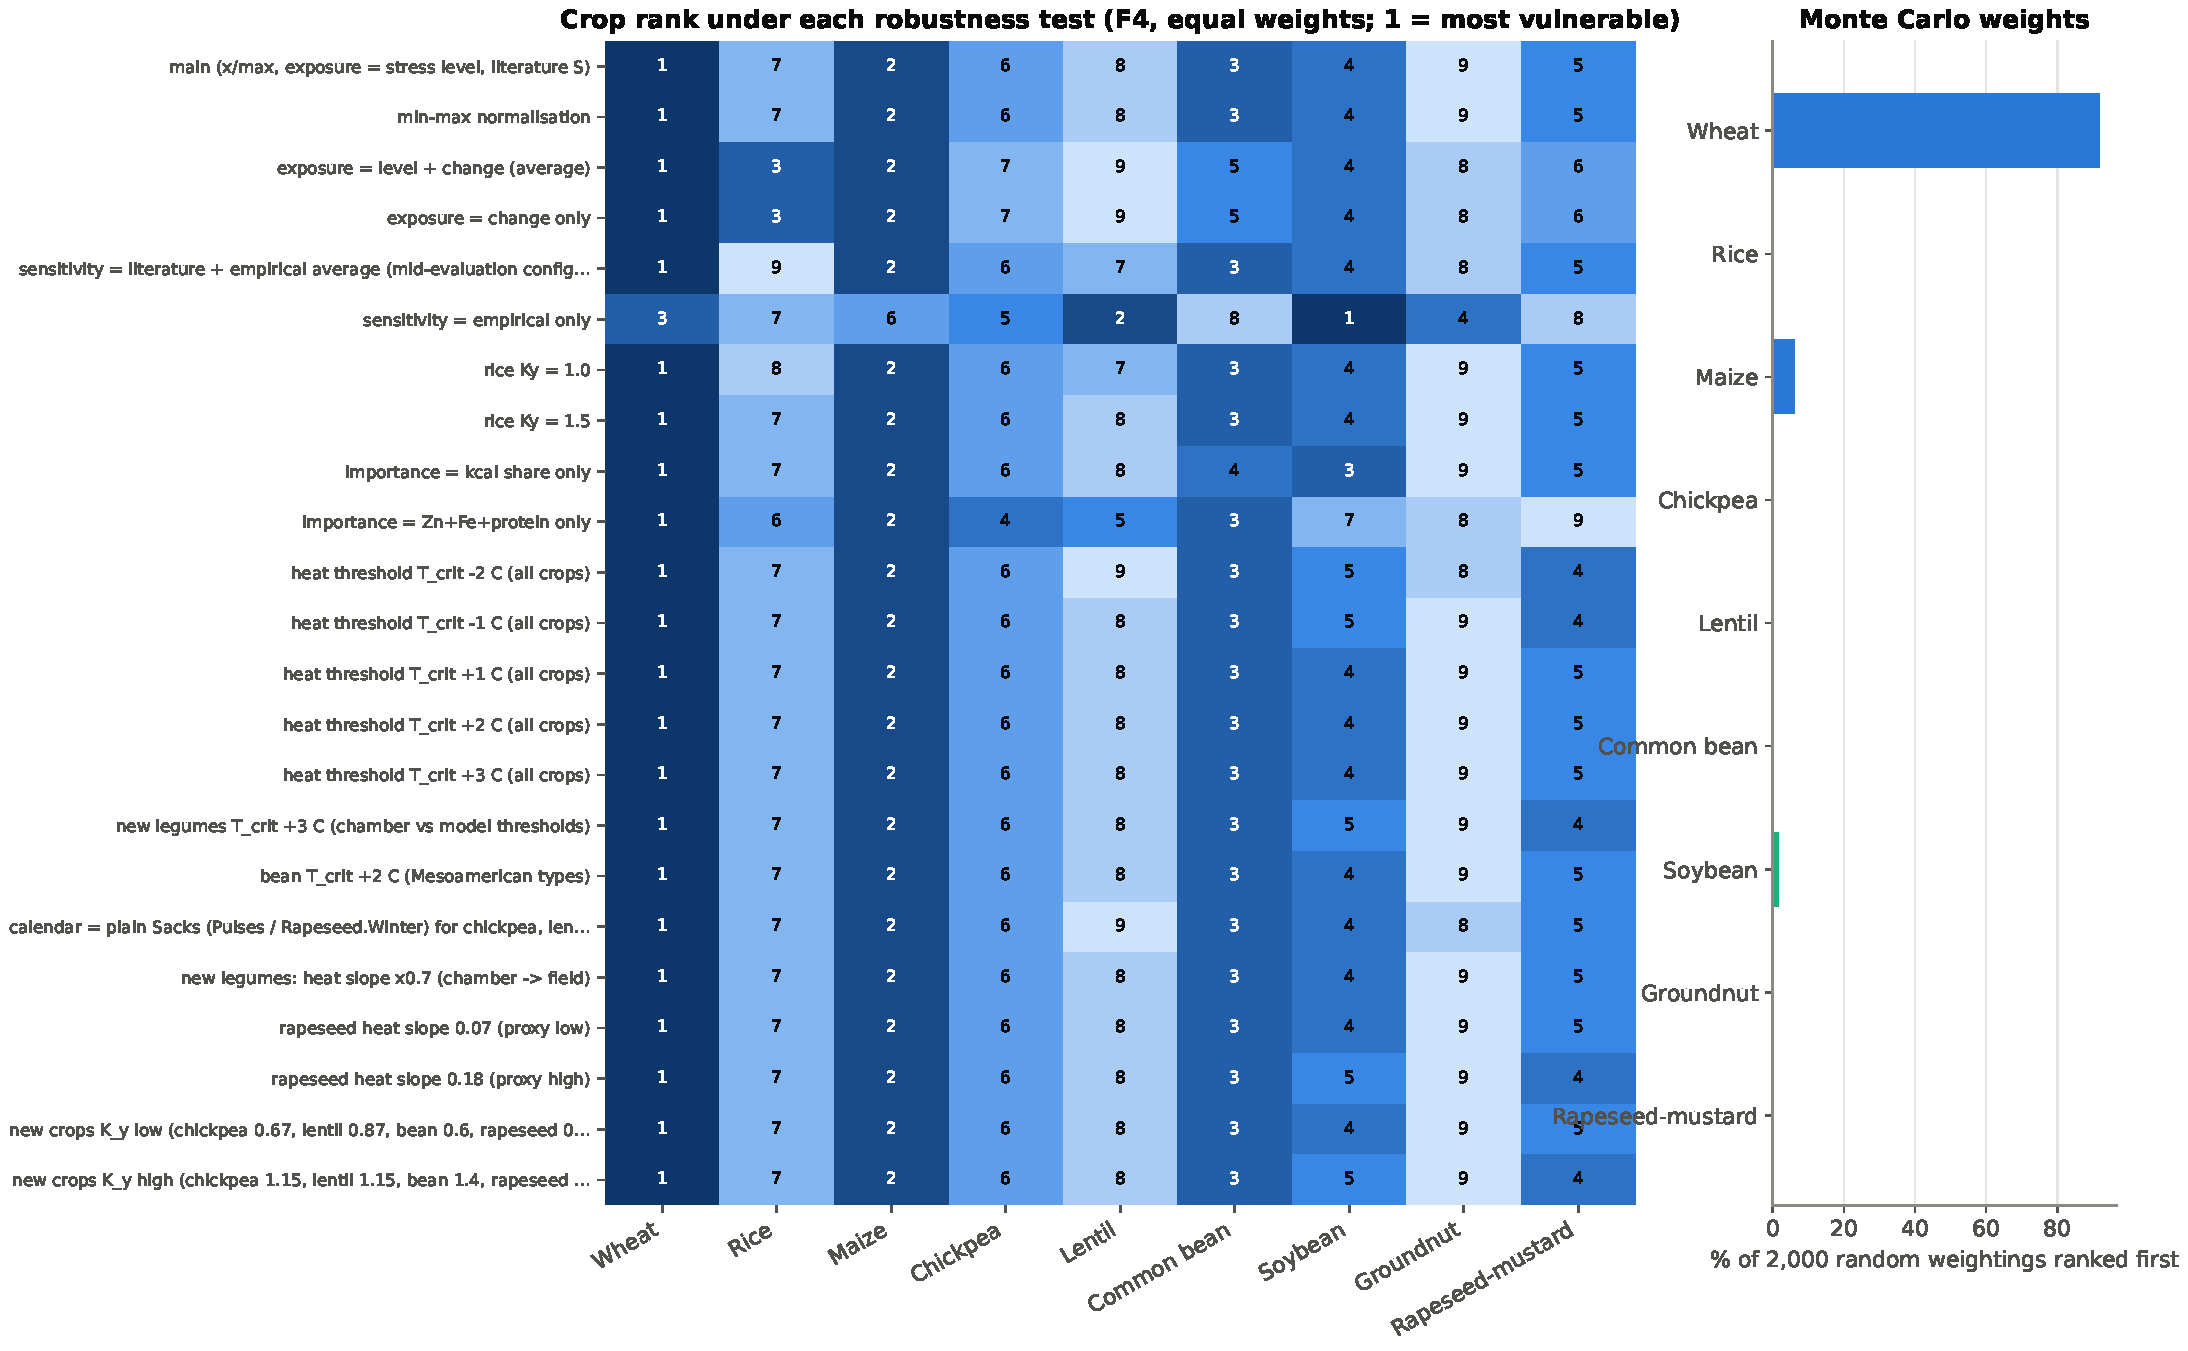
\includegraphics[width=\linewidth]{G10_robustness.pdf}
\caption{Robustness: crop ranks under each one-at-a-time test (left) and shares of first place under random
weightings (right).}\label{fig:robust}\end{figure}

\subsection{Validation against observations}
\begin{itemize}
\item \textbf{Zhao et al.\ (2017).} Against their per-degree global yield losses, the climate part of the index has
Spearman $\rho$ = \zhaoRhoClimate\ and the full index \zhaoRhoFfour. With four crops only, this is descriptive.
\item \textbf{Yield shocks, 2001--2024.} Across the \shockNpairs\ pairs, the climate part is positively
associated with how often yield fell more than one standard deviation below trend ($\rho$ = \shockRho, one-sided
permutation $p$ = \shockP).
  \begin{itemize}
  \item At the mid-evaluation, with 26 pairs, this test was null. That null result is kept on record.
  \item The nine-crop result is an association in a larger and more varied sample, not proof that the index
  predicts shocks.
  \end{itemize}
\item \textbf{Year-to-year anomalies.} The fitted climate response correlates positively with observed 2001--24
yield anomalies in \oosPos\ of \oosN\ pairs with enough data (median $r$ = \oosMedian).
\item \textbf{Future responses.} The literature and empirical future yield responses agree in sign for only
\fySameSign\% of pairs (Section~\ref{sec:futurenut}). This is a disagreement, not a validation.
\end{itemize}

\subsection{Comparison with published studies}
Section~\ref{sec:futurelit} extends this comparison to future-impact studies for all nine crops and reports where
none was found. The earlier comparison of \litN\ findings (Table~\ref{tab:lit}) is kept: \litAgree\ agree,
\litPartial\ partly agree, \litDiffer\ differ and \litOther\ are not directly comparable or add a pathway (the Ray et
al.\ row, which concerns climate-explained variability and not vulnerability, was moved here in the November audit).
These counts say how the evidence is distributed, not how accurate
the model is; several of the studies supply inputs we use (for example \citealp{deryng2014}), so agreement with them is
not independent. The disagreements are informative:
\begin{itemize}
\item \citet{lobell2011} attribute Russian wheat losses to temperature, while our monthly threshold measure sees
mainly rainfed water deficit there;
\item maize suitability studies \citep{ramirez2017} project losses in Africa where our single climate model projects
a wetter South African growing season.
\end{itemize}
Each published value is checked against its source (quote, page or table, read level) in
\file{docs/evidence/literature\_comparison\_sources.md}. Only signs and rank orders are compared, never index values with
yield percentages.

\begin{table}[p]\centering\scriptsize
\caption{Our results next to published findings (verdicts computed from our result tables by
\file{code/22\_literature\_comparison.py}).}\label{tab:lit}
\begin{minipage}{\textwidth}\centering
\adjustbox{max width=\textwidth}{\begin{tabular}{p{0.9cm}p{3.0cm}p{4.4cm}p{4.6cm}p{2.0cm}}
\toprule
 & Study & Published finding & Our comparable result & Verdict \\
\midrule
Z1 & Zhao et al. 2017 PNAS & yield change per +1 C: maize -7.4, wheat -6.0, rice -3.2, soybean -3.1 (n.s.) -$>$ maize $>$ wheat $>$ rice $>$ soybean & climate part E x S (equal weights): maize $>$ wheat $>$ soybean $>$ rice; Spearman rho with Zhao = +0.8 (n = 4) & agree (order of maize, wheat) \\
Z2 & Zhao et al. 2017 PNAS (Fig. 3) & wheat loss per +1 C: India -9.1, Russia -7.8, USA -5.5, China -2.6 \% & wheat heat exposure E\_heat: India 0.115, Russia 0.015, USA 0.015, China 0.002 & agree (heat) \\
L1 & Lobell, Schlenker \& Costa-Roberts 2011 Science & Russia wheat production about -15 \% from temperature trends & wheat-Russia F4 = 0.1315 (top pair); heat part 0.0027 vs water part 0.1288 & differ (mechanism) \\
R1 & Ray et al. 2015 Nat. Commun.; Ray et al. 2019 PLoS ONE & climate explains 32-39 \% of yield variability; rice least & rice climate part E x S = 0.0247, lowest of the four (wheat 0.1077, maize 0.1345, soybean 0.0830) & not directly comparable (different outcome) \\
D1 & Deryng et al. 2014 ERL (Table 1) & maize -10.5, wheat -10.1, soybean -6.9 \% (RCP4.5 with CO2: -4.9, +13.0, +10.8) & our conditional yield change (mean over countries, no CO2): maize -2.5 \%, wheat -3.5 \%, soybean +0.7 \% & sign agrees for maize; sign agrees for wheat; sign differs for soybean; our magnitudes smaller \\
C1 & Challinor et al. 2014 Nat. Clim. Change & $>$ 70 \% of projections show yield losses & 76 \% of our 59 pairs show a climate-driven yield loss (literature accounting); cereals only: 74 \% & agree \\
RC & Ramirez-Cabral et al. 2017 Sci. Rep. & suitable area: Africa -7 to -11 \%, South America -5 \%, India marginal areas become unsuitable & maize change in F4 2041-60 vs 1971-2000: South Africa -0.0127, Brazil +0.0019, India -0.0002 & differ \\
RP/HU & Rippke et al. 2016 Nat. Clim. Change; Hummel et al. 2018 Sci. Rep. & beans -10 \% area needing transformation in Uganda/Tanzania by the 2050s (RP); most SE African bean areas unsuitable by 2040-69, drought-driven (HU) & bean-Tanzania F4 change +0.0188; conditional yield change -17.7 \% & agree (direction) \\
Q1 & Qian et al. 2019 ERL (Table 2) & -0.8 to -5.7 \% production at +2 C with CO2 fixed (+3 to +11 \% with CO2) & rapeseed-Canada conditional yield change -3.2 \% (no CO2); flowering T\_eff change +3.1 C & agree (sign) \\
K1 & Kalra et al. 2008 Curr. Sci. & yields fall with warmer seasons: chickpea -0.53 to -3.01, mustard -0.92 to -2.01 q/ha per C & India 2041-60: chickpea T\_eff +1.3 C, yield -0.2 \%; rapeseed-mustard T\_eff +1.6 C, yield -2.2 \% & agree (sign) \\
BE/NE & Beach et al. 2019 Lancet Planet. Health; Nelson et al. 2018 Nat. Sustain. & South Asia iron availability below the recommended intake; micronutrients, not calories, are the binding constraint & India 2021-23 iron supply / requirement = 0.89 (15 \% bioavailability: 1.00); energy 1.00, protein 1.00 & agree (main requirement) \\
M1 & Myers et al. 2014 Nature & iron concentration: wheat -5.1, rice -5.2, soybean -4.1 \% (significant) & applied to India's 2021-23 iron supply shares, these declines alone would lower national iron supply by 2.2 \% (an additional pathway the index excludes) & additional pathway \\
\bottomrule
\end{tabular}
}
\par\vspace{2pt}{\footnotesize Signs and rank orders only; published values verified in docs/literature\_comparison\_sources.md; ours computed by code/22\_literature\_comparison.py.}
\end{minipage}

\end{table}

\section{Scientific limitations and uncertainty}\label{sec:limits}
Each limitation is tied to the result it affects. Where it was tested, the test is named.

\subsection{Climate measurement}
\begin{itemize}
\item \textbf{Monthly data hide hot days.} Heat exposure is a lower bound. Rice and soybean score near zero on heat
largely for this reason: their thresholds are defined for short exposures that monthly means cannot show. The
direction of bias is to understate heat vulnerability, most for crops with high thresholds.
\item \textbf{The water ratio has no soil storage or runoff, and treats irrigation as unlimited.}
  \begin{itemize}
  \item It overstates stress for crops grown on stored soil moisture. Rabi chickpea in India is grown on residual
  monsoon moisture, and it sets the water reference.
  \item It understates stress where irrigation water is itself at risk.
  \end{itemize}
  The index therefore assumes irrigation keeps flowing. This matters most for rice and for Telangana.
\item \textbf{Station coverage.} In cell-months without stations, CRU-TS returns climatology, which damps rainfall
variability.
\end{itemize}

\subsection{Crop parameters}
The ledger (Appendix~\ref{app:ledger}) labels every value as published, derived or proxy, and
Section~\ref{sec:parevidence} audits \parNRows\ register rows: \parNPublished\ published, \parNDerived\ derived,
\parNBorrowed\ borrowed, \parNAssumption\ assumptions and \parNUnsupported\ unsupported (the rapeseed heat slope; the
rice heat slope is also unsupported as a yield slope). The ``tested'' ranges below are exploratory perturbations, not
literature-supported uncertainty ranges.
\begin{itemize}
\item \textbf{New legumes are fitted.} Their thresholds and slopes are fits to chamber or pot experiments on one
to three genotypes. Chamber exposure is continuous and without recovery days, so these values probably overstate
field sensitivity. They also sit below model-calibrated thresholds such as those used for wheat, maize and soybean.
Exploratory perturbation: $T_{\text{crit}}+3$\,\si{\celsius} and slopes $\times0.7$ (the direction is supported, the
size is not); wheat stays first.
\item \textbf{Common bean.} The threshold comes from one heat-susceptible Andean cultivar. It is applied to FAO
``beans, dry'', which in India and Myanmar include tropical \emph{Vigna} pulses. Because bean in India sets the heat
reference for all crops, this choice scales every heat exposure; with the India and Myanmar bean pairs removed the
heat reference falls by a factor of \scrHeatRatio\ (Section~\ref{sec:parevidence}). Exploratory perturbation: $+2$\,\si{\celsius}.
\item \textbf{Rice.} FAO gives no rice $K_y$ (FAO-33 classes rice only as ``high'' sensitivity, like maize), so
maize's 1.25 is a proxy. Rice's heat slope is a spikelet-fertility slope, not a yield slope, and is unsupported as
one. Exploratory perturbation: $K_y$ 1.0 and 1.5.
\item \textbf{Rapeseed-mustard.} The threshold is converted from a daily-maximum threshold with an assumed diurnal
range. No published heat slope was found, so wheat's is borrowed and unsupported; it is perturbed from 0.07 to 0.18. The FAO-56 Rev.1
$K_y$ of 0.90 is tabulated without a stated source. Parameters from \emph{B.~napus} probably overstate the heat
sensitivity of Indian mustard (\emph{B.~juncea}).
\item \textbf{Inaccessible sources.} Not read in full: \citet{prasad2002bean}, \citet{prasad2003peanut} and
\citet{morrison2002} (closed access). Their values are taken from abstracts and from \citet{boote2005}.
\end{itemize}

\subsection{Maps, calendars and panels}
\begin{itemize}
\item \textbf{Crop maps are from 2010 (SPAM).} Areas have since moved; Telangana's paddy area is about three times
the 2010 map.
\item \textbf{Calendars.} Calendars are partly gap-filled. Chickpea, lentil and rapeseed use the cool-season rule,
whose plain-Sacks alternative is tested.
\item \textbf{Panels.} Panels sample the main producers (half to nine-tenths of world output), not all countries.
Pigeon pea (tur) and moong, major pulses in South India, are not among the nine crops.
\end{itemize}

\subsection{Nutrition}
\begin{itemize}
\item \textbf{Supply, not intake.} National supply is not individual intake, and composition is one value per item.
Whole-grain and primary-weight compositions overstate zinc and iron.
\item \textbf{Requirements.} RNIs compared with mean supply overstate shortfall at the individual level. The iron
result changes with the bioavailability assumption (\nIronShort\ countries short under the main requirement, none
under the alternative).
\item \textbf{Shock accounting.} There is no price or trade response, so the upper bound is a bound, not a forecast.
\end{itemize}

\subsection{Future}
\begin{itemize}
\item \textbf{One model, one scenario.} The future results show direction under MRI-ESM2-0 SSP2-4.5, not the range
of plausible futures. Regional rainfall changes in particular are model-dependent.
\item \textbf{Fixed area, calendars, irrigation and diets}, with no CO$_2$ fertilisation and no adaptation. Elevated
CO$_2$ would raise yields of C$_3$ crops but lower their zinc, iron and protein \citep{myers2014}. The yield effect is
not included. The concentration effect is not in the main results either; it is reported only as a separate
experimental stress test with partial coverage (Section~\ref{sec:co2}) and must not be read as a forecast.
\item \textbf{Response methods disagree.} The literature and empirical future yield responses disagree for about
half the pairs, so the future nutrient numbers are conditional screening estimates.
\end{itemize}

\subsection{Index design}
\begin{itemize}
\item \textbf{Our combination rules.} Pairing, equal nutrient weights, normalisation by the maximum, and equal or
production weighting across countries are our design choices. Robustness tests show their effect but cannot show
that they are right.
\item \textbf{Relative values.} F4 values are meaningful as relative positions within this set of crops and
countries. Adding crops changes the reference and hence every value, as the four-to-nine-crop comparison showed.
\end{itemize}

\section{Discussion and conclusions}\label{sec:discussion}

\subsection{What the index indicates}
An index is only useful if a high value means something one can act on. A high \Fd\ marks a crop and place where
three things coincide:
\begin{itemize}
\item the growing area is already under heat or water stress;
\item the crop loses yield quickly under that stress;
\item people depend on the crop for nutrients.
\end{itemize}
Read this way, the results say five things.
\begin{enumerate}
\item \textbf{The most vulnerable crop is not the most heat-sensitive one.} Soybean has the steepest literature heat
slope, yet ranks low: its monthly flowering temperature stays below its threshold, and it is eaten mainly as oil.
Wheat is only moderately sensitive, but it is grown in the hottest and driest plains of the panel and is the
largest single food source of zinc and iron in most panel countries. Vulnerability is about \emph{overlap}, which
neither a yield study nor a nutrient study shows on its own.
\item \textbf{The nutrient at stake is iron.} Iron is the only nutrient whose national supply falls below the main
requirement in any panel country (\nIronShort\ of \nAdqCountries). The crops that supply most iron are among those
whose climate stress is highest or rising fastest: wheat everywhere, and pulses in South Asia and East Africa.
Climate risk therefore falls on a nutrient that is already short, not on calories. This rests on the requirement
chosen (Section~\ref{sec:adequacy}).
\item \textbf{Concentrated diets amplify the signal.} Where a few crops supply most nutrients, a loss in one
vulnerable crop removes a larger share of a nutrient. India, for example, gets \divIndIronTopShare\% of its iron from
wheat, and its energy supply is spread over an effective \divIndKcal\ food items against \divWorldKcal\ for the
world as a whole.
\item \textbf{Irrigation is the hidden buffer.} Rice scores low largely because most of its area is irrigated,
which the water measure counts as unstressed. Groundwater depletion or reservoir shortfalls would move rice up the
ranking, and monthly data cannot see the hot days that matter for rice.
\item \textbf{The future changes magnitudes more than the order.} Under one model and one scenario, the crop
ranking in 2041--2060 is largely the same, but vulnerability rises for wheat and common bean. The increase comes
mostly from heat, while today's scores come mostly from water. Pulses, a key protein and iron source for
vegetarian diets, rise fastest relative to their present level (\grpPulsePct\%).
\end{enumerate}

\subsection{What it points to}
As a screening tool, the index points to where adaptation would protect most nutrition:
\begin{itemize}
\item \textbf{wheat in India:} the present score is mainly water, but the projected increase comes almost entirely
from heat during flowering, so heat tolerance and sowing dates matter as well as water;
\item \textbf{wheat in Russia:} both today's score and most of the projected increase are water-driven;
\item \textbf{wheat in the USA:} the increase is shared between heat and water;
\item \textbf{rainfed maize in southern Africa:} drought management;
\item \textbf{beans in tropical Brazil and East Africa:} heat-tolerant varieties;
\item \textbf{on the demand side:} diversifying iron sources, so that one crop's bad year does not decide iron
supply.
\end{itemize}
These are directions suggested by where scores are high, not tested interventions.

\subsection{What the four extensions add}
\begin{itemize}
\item \textbf{Parameter evidence (Section~\ref{sec:parevidence}).} The headline survives the audit but its scope
narrows. Wheat is first in the full index and also first among the seven crops whose parameters are supported, but
rice and rapeseed cannot be placed on supported heat parameters, and bean in India and Myanmar does not match its
parameter source. The full nine-crop ranking is therefore an \emph{assumption-dependent} result.
\item \textbf{Future literature (Section~\ref{sec:futurelit}).} Direction and mechanism agree with published studies
where they are most comparable (wheat in India, beans in Tanzania, mustard in India) and differ where studies include
CO$_2$ fertilisation or adaptation, or where our index cannot see the mechanism (rice, irrigated crops, season
shortening). The studies include evidence that challenges rising vulnerability, and the one climate model we use is
described by one study as the least pessimistic.
\item \textbf{CO$_2$ and nutrient quality (Section~\ref{sec:co2}).} The concentration channel, as an experimental
stress test with partial coverage, lowers national zinc by more than the climate yield channel in all
\cotwoNCountries\ panel countries and iron in \cotwoNQualGtQtyIron, and does so even where the climate scenario removes no
modelled supply. Calories are not estimated. Nothing here is a forecast.
\item \textbf{Diversity after losses (Section~\ref{sec:divloss}).} Losing part of a dominant staple lowers total
supply and can raise the effective number of food sources. Diversity must be read with total supply and adequacy,
never alone.
\end{itemize}

\subsection{Supported conclusions and their strength}
\begin{table}[H]\centering\small
\caption{Conclusions and how strongly the evidence supports them.}\label{tab:conclusions}
\begin{tabular}{p{6.3cm}p{2.0cm}p{6.4cm}}
\toprule
Conclusion & Support & Evidence and caveat \\
\midrule
Wheat is the most vulnerable of the nine crops & strong, conditional & first in \robTopFfour/\robNFfour\ F4 robustness rankings and \mcTopShare\% of random weightings; exceptions only under empirical-only sensitivity. Conditional on proxies: first among the seven crops with supported parameters (rice and rapeseed unavailable) \\
Order of positions 2--9 & weak & moves with weighting and pulse parameters \\
Rice and rapeseed positions & not established & heat slopes unsupported; present scores are almost entirely water \\
Direction of future change agrees with published studies where comparable & moderate, partial & wheat in India, bean in Tanzania, mustard in India; differs where CO$_2$ or adaptation is included; \litNPairsNoStudy\ of \litNPairs\ pairs have no study \\
Elevated-CO$_2$ quality channel lowers zinc, iron and protein & stress test only & covered crops only, no energy or fat, experiment-based step, hybrid reference; not a forecast \\
Crop loss can raise food-source diversity while lowering supply & strong (arithmetic) & predicts the sign in every single-item case; read with adequacy \\
Water dominates today's scores, heat the projected increase & moderate & \presentWaterShare\% water today, \futHeatShare\% heat in the change; water ratio has no soil storage; one climate model \\
Iron is the nutrient closest to shortfall & conditional & \nIronShort/\nAdqCountries\ countries under the main requirement, \nIronShortAlt\ under the alternative \\
Index associated with yield-shock frequency & weak & positive in 59 pairs, null in the 26-pair mid-evaluation sample; association only \\
Future yield and nutrient losses & screening only & literature and empirical responses disagree for about half the pairs \\
Hyderabad's risk is more structural than climatic & moderate & district anaemia with adequate energy; rice irrigated; based on state-urban and district data, not city intake \\
\bottomrule
\end{tabular}
\end{table}

\subsection{Conclusion}
Across nine crops, the Climate--Nutrition Vulnerability Index identifies \MakeLowercase{\topEq} as the crop whose
climate stress most overlaps with its nutritional role. This holds across \robTopFfour\ of \robNFfour\ robustness
rankings and is stable to 2041--2060 under one climate model. Cereals as a group are most vulnerable, pulses rise
fastest, and the nutrient most at stake is iron. For India the index points to wheat, chickpea and common bean; for
Hyderabad it points to a rice-based diet whose main problem, iron density, exists independently of climate. The
index is most useful as a map of where climate stress and dietary dependence coincide, which is where adaptation
and diet diversification would protect nutrition most. It is not a forecast of yields or diets.

The audit of parameters, the comparison with future-impact studies, the CO$_2$ stress test and the diversity analysis
sharpen this reading without overturning it. Wheat's first place does not depend on the unsupported parameters, but the
positions of rice and rapeseed cannot be established with them, several studies that include CO$_2$ fertilisation or
adaptation project gains where we project losses, quality changes in grain compound the quantity loss for zinc, iron
and protein, and a loss in a dominant staple can make food sources look more even while supply falls. None of this
means the model is the most accurate available; the unresolved evidence gaps are listed in
Sections~\ref{sec:parevidence}--\ref{sec:co2} and the human review tasks in Section~\ref{sec:repro}.

\section{Reproduction and audit}\label{sec:repro}

\subsection{How to reproduce the results}
\paragraph{Environment.} Python 3.13 with the pinned packages in \file{requirements.txt}. Python 3.14 is not
supported, because rasterio builds from source. The PDFs are compiled with Tectonic. The documents are ASCII-only
and select \texttt{inputenc}/\texttt{fontenc} under pdfLaTeX, but the pdfLaTeX route has not been tested.

\paragraph{Raw data.} Put the raw files in \file{data/raw/} and check them against the manifest:
\begin{verbatim}
py -3.13 -m venv .venv
.venv\Scripts\python -m pip install -r requirements.txt
cd code
..\.venv\Scripts\python 00_data_manifest.py --check
powershell -ExecutionPolicy Bypass -File .\run_all.ps1
\end{verbatim}

\paragraph{Pipeline.} \file{run\_all.ps1} runs, in order:
\begin{enumerate}
\item downloads (skipping files present);
\item K\"oppen groups;
\item crop grids;
\item monthly climate series (precipitation, $T_{\max}$, $T_{\text{mean}}$);
\item hazards;
\item future climate;
\item for each of the four-crop and nine-crop runs: panels, country series, sensitivity checks, nutrition, index
and robustness, yield-to-diet, validation and literature sensitivity;
\item the mid-evaluation figure set for the four-crop run;
\item future index, future yield and nutrition, run comparisons, figures, input register, India and Hyderabad
analysis, literature comparison, source register;
\item the consistency checks (\file{24\_checks.py}) and parameter fits (\file{25\_parameter\_fits.py});
\item the LaTeX tables and macros (\file{19\_endeval\_tex.py}, \file{26\_report\_tables.py});
\item the documents.
\end{enumerate}
Any script that fails, any failed check and any failed document compile stops the run, so stale results cannot be
compiled as new ones. On the audit machine the full run from raw inputs, climate steps included, took about 21
minutes; downloading the raw data takes much longer. The switch \texttt{-SkipClimate} reuses \file{data/work}.

\subsection{Audit of 18 November 2026}
\paragraph{Inputs.} The manifest check found all \manifestFiles\ raw files present with matching SHA-256 checksums.
The 55 files of the mid-evaluation and end-evaluation snapshots were listed before. The 19 files of the
Telangana mask and the Indian surveys, already used by the analysis, were added to the manifest in this audit
without changing any existing entry. The climate, SPAM, calendar, FAOSTAT and USDA files are the original
snapshot files, so this is an exact reproduction, not a new data snapshot.

\paragraph{Full rerun.} The previous intermediate files (\file{data/work}, about 10\,GB) and outputs were moved
aside as a comparison copy, so no cached file could be reused. The whole pipeline, including every climate step,
was then run from the raw inputs in a fresh Python 3.13 environment built from \file{requirements.txt}.

\paragraph{Comparison.} \file{code/27\_compare\_rerun.py} compared every regenerated file with the previous copy
(absolute and relative tolerance $10^{-9}$). Of \auditFiles\ files:
\begin{itemize}
\item \auditIdentical\ are identical;
\item \auditWithinTolerance\ are within tolerance;
\item \auditDiffers\ differ;
\item \auditNew\ are new outputs of this audit.
\end{itemize}
The \auditMissing\ files of the previous copy that were not regenerated are all unused by the pipeline:
\begin{itemize}
\item 72 per-cell climate metric files of the rice-only prototype, written only when
\texttt{CNVI\_LEGACY\_METRICS=1} and read by no script;
\item an old production cache, renamed since;
\item a leftover pulse cache and a shell script.
\end{itemize}
\textbf{Every output present in both runs is identical}, so the full rerun reproduces all previous results exactly
(Table~\ref{tab:auditsummary}; the file list is in Appendix~\ref{app:audit}). The pipeline also stopped as designed
on its first attempt: the report compile failed because this audit's macros did not yet exist, and nothing was
built from stale results.

\begin{table}[H]\centering\small\caption{Rerun from raw inputs compared with the previous outputs.}\label{tab:auditsummary}
\begin{tabular}{lrrr}
\toprule
Output area & identical & new & missing \\
\midrule
data/processed & 85 & 1 & 0 \\
data/work & 107 & 0 & 75 \\
docs/four\_crop/generated & 13 & 0 & 0 \\
docs/nine\_crop/generated & 18 & 11 & 0 \\
\bottomrule
\end{tabular}

\end{table}

\paragraph{Checks.} \checksPassed\ of \checksN\ consistency checks pass on the regenerated results
(Table~\ref{tab:checks}). The derived heat parameters of the new crops are refitted from the published data by
\file{code/25\_parameter\_fits.py} and reproduce \file{config.py} (Table~\ref{tab:fits}).

\paragraph{What was not done.}
\begin{itemize}
\item No pdfLaTeX compile.
\item No independent teammate review of parameters, calculations or interpretation.
\item No team rehearsal.
\item No re-download of FAOSTAT. A fresh download would be a new data snapshot and would change the numbers
slightly.
\end{itemize}


\clearpage
\bibliography{refs}

\clearpage
\appendix
\section{Parameter and source ledger}\label{app:ledger}
Table~\ref{tab:ledger} records, for every parameter that enters the index or the nutrition accounting:
\begin{itemize}
\item its value and exact source location;
\item the experiment behind it;
\item the temperature metric and the outcome measured;
\item whether the value is published, derived by us, or a proxy;
\item the alternatives tested.
\end{itemize}
Verbatim quotes and read levels are in \file{docs/literature\_verification\_new\_crops.md} (new crops, including the
follow-up checks of this audit in its Section~8) and in the mid-evaluation verification notes (original crops).

\paragraph{Read levels.} Full texts were read for:
\begin{itemize}
\item \citet{bhandari2020}, \citet{boote2005}, \citet{tari2022};
\item FAO-33, FAO-66, FAO-56 and FAO-56 Rev.1;
\item WHO/FAO 2004;
\item the Deryng, Yoshida and Jagadish sources.
\end{itemize}
Only abstracts were available for \citet{prasad2002bean}, \citet{prasad2003peanut}, \citet{morrison2002},
\citet{nandi2021} and \citet{istanbulluoglu2010}. The chickpea $K_y$ range 0.67--0.93 attributed to Jalota et al.\
(2006) is known only through a secondary citation; that study's abstract gives no $K_y$.

\paragraph{Derived heat parameters.} The derived thresholds and slopes are refitted from the published data by
\file{code/25\_parameter\_fits.py} (Table~\ref{tab:fits}). The model is the Deryng broken-stick function
$\text{loss} = \min(1, s_T\max(0,\Teff-\Tcrit))$, fitted by least squares on a grid. Chamber day/night regimes
$D/N$ are converted with $\Teff = ((D+N)/2 + D)/2$.

{\scriptsize\begin{longtable}{L{0.091}L{0.098}L{0.098}L{0.171}L{0.183}L{0.140}L{0.122}L{0.098}}
\caption[Parameter and source ledger]{Parameter and source ledger. Values are read from \texttt{code/config.py}. Status: published = value printed in the source; DERIVED = our arithmetic or fit on published values; PROXY = value borrowed from another crop, outcome or metric. Read levels and verbatim quotes: \texttt{docs/literature\_verification\_new\_crops.md}.}\label{tab:ledger}\\
\toprule
Crop & Parameter & Value & Source and location & Experiment / conditions & Metric and outcome & Status & Alternatives tested \\
\midrule\endfirsthead
\toprule
Crop & Parameter & Value & Source and location & Experiment / conditions & Metric and outcome & Status & Alternatives tested \\
\midrule\endhead
\bottomrule\endfoot
Rice & $T_{crit}$ & 35.0 & \citet{yoshida1981} Table 2.4; FAO-66 p.~106 & critical high temperature at anthesis, $>$1 h & daily mean air $T$; spikelet sterility & published (metric differs from $T_{eff}$) & $\pm$1--3\,\si{\celsius} \\
Rice & $s_T$ & 0.070 & \citet{jagadish2007} & IR64 in chambers, $\le$1 h at anthesis & spikelet fertility ($\approx$7\%/\si{\celsius} above 29.6\,\si{\celsius}) & published, outcome borrowed (fertility $\to$ yield) & -- \\
Rice & $K_y$ & 1.25 & FAO-33 Table 2 p.~7 (rice ``high'', no number); maize value FAO-66 Table 1 & -- & seasonal yield--ET response & PROXY (maize) & 1.0, 1.5 \\
Wheat & $T_{crit}$, $T_{lim}$ & 25, 35 & \citet{deryng2014} Table A.1 & PEGASUS model, spring wheat & $T_{eff}$, 45--70\% of season; yield & published model parameter (also used for winter wheat) & $\pm$1--3\,\si{\celsius} \\
Wheat & $K_y$ & 1.10 & FAO-66 Table 1 (spring 1.15, winter 1.05) & -- & seasonal & DERIVED mean of two FAO values & -- \\
Maize & $T_{crit}$, $T_{lim}$ & 32, 45 & \citet{deryng2014} Table A.1 & PEGASUS model & $T_{eff}$; yield & published model parameter & $\pm$1--3\,\si{\celsius} \\
Maize & $K_y$ & 1.25 & FAO-66 Table 1 (= FAO-33) & -- & seasonal & published & -- \\
Soybean & $T_{crit}$, $T_{lim}$ & 35, 40 & \citet{deryng2014} Table A.1 & PEGASUS model & $T_{eff}$; yield & published model parameter & $\pm$1--3\,\si{\celsius} \\
Soybean & $K_y$ & 0.85 & FAO-66 Table 1 (= FAO-33) & -- & seasonal & published & -- \\
Chickpea & $T_{crit}$, $s_T$ & 34.0, 0.140 & \citet{bhandari2020} Table 3 p.~749 & 3 Indian genotypes, pots, growth chambers 30/20--42/32\,\si{\celsius} (12/12 h), flowering to maturity & seed yield per plant & DERIVED fit (5 points) & $T_{crit}$ 30.3 (pod set, \citealp{devasirvatham2013}); +3\,\si{\celsius}; slope $\times$0.7 \\
Chickpea & $K_y$ & 0.88 & \citet{tari2022} p.~143 & field, Konya (Turkey), 2 years, 2 sowing dates & seasonal (0.85, 0.91) & DERIVED mean of 2 field values; not in FAO & 0.67, 1.15 \\
Lentil & $T_{crit}$, $s_T$ & 31.9, 0.170 & \citet{bhandari2020} Table 3 & 2 Indian genotypes, as chickpea & seed yield per plant & DERIVED fit (4 points, 2 parameters) & +3\,\si{\celsius}; slope $\times$0.7 \\
Lentil & $K_y$ & 1.00 & \citet{nandi2021} abstract & field, Lower Gangetic Plain, after rice & ``1\% yield loss per 1\% decline in relative ET''; best treatment 0.87 & PROXY (abstract only) & 0.87, 1.15 \\
Common bean & $T_{crit}$, $s_T$ & 25.5, 0.111 & \citet{prasad2002bean} via \citet{boote2005} p.~470 & cv.\ Montcalm (Andean red kidney), sunlit chambers, season-long, 10\,\si{\celsius} diurnal range & seed yield (max at 28/18, zero at 37/27\,\si{\celsius}) & DERIVED from two published points; full text not read & $T_{crit}$ +2\,\si{\celsius}; slope $\times$0.7 \\
Common bean & $K_y$ & 1.15 & FAO-33 Table 24 p.~39; FAO-66 Table 1 & -- & seasonal (IAEA field 0.59, 1.43) & published & 0.6, 1.4 \\
Groundnut & $T_{crit}$, $s_T$ & 31.8, 0.095 & \citet{prasad2003peanut} abstract & cv.\ Georgia Green, sunlit chambers 32/22--44/34\,\si{\celsius}, season-long, ambient CO$_2$ & seed yield ($-$14, $-$59, $-$90\%) & DERIVED fit (4 points); full text not read & 29.0/0.074 \citep{boote2005}; +3\,\si{\celsius}; slope $\times$0.7 \\
Groundnut & $K_y$ & 0.70 & FAO-33 Table 24; FAO-66 Table 1 & -- & seasonal & published & -- \\
Rapeseed-mustard & $T_{crit}$ & 26.5 & \citet{morrison2002} abstract & field, Ottawa, 3 years $\times$ 3 sowing dates, 3 \emph{Brassica} species incl.\ \emph{B.~juncea} & accumulated daily $T_{\max}$ above 29.5\,\si{\celsius} at flowering; seed yield & PROXY conversion to $T_{eff}$ with an assumed 12\,\si{\celsius} diurnal range & $\pm$1--3\,\si{\celsius} \\
Rapeseed-mustard & $s_T$ & 0.10 & borrowed: \citet{deryng2014} spring-wheat span (10\,\si{\celsius}) & -- & -- & PROXY (no published slope found) & 0.07, 0.18 \\
Rapeseed-mustard & $K_y$ & 0.90 & FAO-56 Rev.1 Table 8.7 p.~279 \citep{fao56rev1} & no source stated by FAO; field 0.87 \citep{istanbulluoglu2010} & seasonal & published, origin not traceable & 0.85, 0.95 \\
Rice & $K_c$ ini, mid, end; $\bar K_c$ & 1.05, 1.20, 0.75; 1.11 & FAO-56 Tables 11--12 \citep{fao56} & subhumid reference conditions & crop water need ($\mathrm{ET_c}=K_c\mathrm{ET_0}$) & published & -- \\
Wheat & $K_c$ ini, mid, end; $\bar K_c$ & 0.40, 1.15, 0.33; 0.88 & FAO-56 Tables 11--12 \citep{fao56} & subhumid reference conditions & crop water need ($\mathrm{ET_c}=K_c\mathrm{ET_0}$) & published & -- \\
Maize & $K_c$ ini, mid, end; $\bar K_c$ & 0.30, 1.20, 0.48; 0.84 & FAO-56 Tables 11--12 \citep{fao56} & subhumid reference conditions & crop water need ($\mathrm{ET_c}=K_c\mathrm{ET_0}$) & published & -- \\
Soybean & $K_c$ ini, mid, end; $\bar K_c$ & 0.40, 1.15, 0.50; 0.89 & FAO-56 Tables 11--12 \citep{fao56} & subhumid reference conditions & crop water need ($\mathrm{ET_c}=K_c\mathrm{ET_0}$) & published & -- \\
Chickpea & $K_c$ ini, mid, end; $\bar K_c$ & 0.40, 1.00, 0.35; 0.77 & FAO-56 Tables 11--12 \citep{fao56}; stages: lentil arid row & subhumid reference conditions & crop water need ($\mathrm{ET_c}=K_c\mathrm{ET_0}$) & published; stages PROXY & -- \\
Lentil & $K_c$ ini, mid, end; $\bar K_c$ & 0.40, 1.10, 0.30; 0.83 & FAO-56 Tables 11--12 \citep{fao56} & subhumid reference conditions & crop water need ($\mathrm{ET_c}=K_c\mathrm{ET_0}$) & published & -- \\
Common bean & $K_c$ ini, mid, end; $\bar K_c$ & 0.40, 1.15, 0.35; 0.85 & FAO-56 Tables 11--12 \citep{fao56} & subhumid reference conditions & crop water need ($\mathrm{ET_c}=K_c\mathrm{ET_0}$) & published & -- \\
Groundnut & $K_c$ ini, mid, end; $\bar K_c$ & 0.40, 1.15, 0.60; 0.85 & FAO-56 Tables 11--12 \citep{fao56} & subhumid reference conditions & crop water need ($\mathrm{ET_c}=K_c\mathrm{ET_0}$) & published & -- \\
Rapeseed-mustard & $K_c$ ini, mid, end; $\bar K_c$ & 0.35, 1.15, 0.35; 0.78 & FAO-56 Tables 11--12 \citep{fao56}; stages: Rev.1 Table 6.11 GDD shares & subhumid reference conditions & crop water need ($\mathrm{ET_c}=K_c\mathrm{ET_0}$) & published; stages PROXY & -- \\
All & Flowering window & 45--70\% of season & \citet{deryng2014} & anthesis at 0.5 of the season & -- & published (model convention) & -- \\
Chickpea, lentil, rapeseed & Calendar & cool-season rule & \citet{sacks2010} (own observed calendar, else wheat/spring-wheat calendar) & Sacks ``Pulses'' calendar is 95\% gap-filled in India and monsoon-season & -- & PROXY (borrowed calendars) & plain Sacks calendar \\
All & $\mathrm{ET_0}$ & Hargreaves & FAO-56 Eq.~52 \citep{fao56} & needs $T_{\max}$, $T_{\min}$, $R_a$ only & -- & published & -- \\
All & Zn requirement & 11.9 mg/d & WHO/FAO 2004 Table 12.4 p.~240 \citep{whofao2004} & adults, low bioavailability (women 9.8, men 14.0) & RNI (upper percentile) & DERIVED mean of two RNIs & 5.95 (moderate) \\
All & Fe requirement & 21.55 mg/d & WHO/FAO 2004 Table 13.5 p.~271 & adults, 10\% bioavailability (women 29.4, men 13.7) & RNI (95th percentile) & DERIVED mean of two RNIs & 14.35 (15\%) \\
All & Energy, protein, fat requirement & ADER; 10\%, 15\% of energy & FAOSTAT food-security indicators; \citet{who2003} & country- and year-specific energy requirement & population average (energy); lower bounds of goals & published & -- \\
All & Zn, Fe composition & per FBS item & USDA SR Legacy \citep{usda2019}; \texttt{code/fbs\_usda\_map.csv} & raw, unprocessed form (whole grain; primary weight) & mg/100 g & mapping choice (overstates Zn, Fe for refined cereals, meat) & -- \\
\end{longtable}}


\begin{table}[H]\centering\small\caption{Derived heat parameters refitted from published data, compared with
\file{config.py} (bean: two published points; rapeseed: converted threshold and borrowed slope).}\label{tab:fits}
\adjustbox{max width=\linewidth}{\begin{tabular}{lp{2.6cm}p{2.6cm}rrrrrc}
\toprule
Crop & $T_{eff}$ points (\si{\celsius}) & relative loss & $T_{crit}$ & $s_T$ & $T_{lim}$ & RMSE & config & match \\
\midrule
Chickpea & 27.5; 32.5; 35.5; 37.5; 39.5 & 0.000; 0.027; 0.219; 0.460; 0.790 & 34.05 & 0.1420 & 41.09 & 0.020 & 34.0 / 0.140 & yes \\
Lentil & 27.5; 32.5; 35.5; 37.5 & 0.000; 0.138; 0.534; 1.000 & 31.85 & 0.1685 & 37.78 & 0.049 & 31.9 / 0.170 & yes \\
Groundnut & 29.5; 33.5; 37.5; 41.5 & 0.000; 0.140; 0.590; 0.900 & 31.75 & 0.0945 & 42.33 & 0.029 & 31.8 / 0.095 & yes \\
Common bean & 25.5; 34.5 & 0; 1 & 25.50 & 0.1111 & 34.50 &  & 25.5 / 0.111 & yes \\
Rapeseed-mustard &  &  & 26.50 & 0.1000 & 36.50 &  & 26.5 / 0.100 & yes \\
\bottomrule
\end{tabular}
}\end{table}

\clearpage
\section{Full result tables}\label{app:tables}

\begin{table}[H]\centering\scriptsize\caption{Country by crop \Fd, 2001--2024.}\label{tab:countrycrop}
\adjustbox{max width=\linewidth}{\begin{minipage}{\textwidth}\centering
\adjustbox{max width=\textwidth}{\begin{tabular}{lrrrrrrrrr}
\toprule
Country & Wheat & Rice & Maize & Chickpea & Lentil & Common bean & Soybean & Groundnut & Rapeseed \\
\midrule
Russia & 0.1315 & -- & -- & 0.0000 & 0.0011 & -- & 0.0036 & -- & -- \\
South Africa & -- & -- & 0.1237 & -- & -- & -- & 0.0137 & -- & $<$0.0001 \\
USA & 0.0903 & $<$0.0001 & 0.0049 & 0.0000 & 0.0003 & 0.0046 & 0.0222 & 0.0017 & 0.0042 \\
India & 0.0676 & 0.0031 & 0.0009 & 0.0273 & 0.0068 & 0.0250 & 0.0002 & 0.0025 & 0.0166 \\
Brazil & 0.0131 & 0.0054 & 0.0137 & -- & -- & 0.0459 & 0.0028 & 0.0005 & $<$0.0001 \\
Tanzania & -- & -- & -- & -- & -- & 0.0357 & -- & -- & -- \\
Ukraine & -- & -- & 0.0332 & -- & -- & -- & -- & -- & -- \\
China & 0.0320 & $<$0.0001 & 0.0016 & 0.0000 & 0.0000 & 0.0004 & 0.0082 & 0.0016 & 0.0018 \\
Canada & -- & -- & -- & -- & 0.0056 & -- & -- & -- & 0.0316 \\
Myanmar & -- & -- & -- & -- & -- & 0.0088 & -- & -- & -- \\
Nigeria & -- & 0.0064 & -- & -- & -- & -- & -- & 0.0012 & -- \\
Australia & -- & -- & -- & 0.0063 & 0.0000 & -- & -- & -- & -- \\
Argentina & -- & -- & -- & -- & -- & -- & 0.0040 & -- & -- \\
Egypt & 0.0036 & -- & -- & -- & -- & -- & -- & -- & -- \\
Turkey & -- & -- & -- & 0.0024 & -- & -- & -- & -- & -- \\
Italy & -- & 0.0015 & -- & -- & -- & -- & -- & -- & -- \\
Ethiopia & -- & -- & -- & 0.0008 & 0.0008 & -- & -- & -- & -- \\
Bangladesh & -- & 0.0003 & -- & -- & -- & -- & -- & -- & -- \\
France & -- & -- & -- & -- & -- & -- & -- & -- & 0.0002 \\
Belarus & -- & -- & -- & -- & -- & $<$0.0001 & -- & -- & -- \\
\bottomrule
\end{tabular}
}
\par\vspace{2pt}{\footnotesize -- = country not in the crop's panel. Values: F4, 2001--2024 stress level, literature-only sensitivity.}
\end{minipage}
}\end{table}

\begin{table}[H]\centering\small\caption{Nutrient adequacy ratios, 2021--23, main and alternative requirements.}\label{tab:adequacy}
\adjustbox{max width=\linewidth}{\begin{tabular}{lrrrrrrrrr}
\toprule
Country & kcal & protein & fat & Zn & Fe & MAR & Zn mod. & Fe 15\% & MAR alt \\
\midrule
Bangladesh & 1.00 & 1.00 & 1.00 & 1.00 & 0.70 & 93.9 & 1.00 & 1.00 & 100.0 \\
South Africa & 1.00 & 1.00 & 1.00 & 1.00 & 0.82 & 96.4 & 1.00 & 1.00 & 100.0 \\
Tanzania & 1.00 & 1.00 & 1.00 & 1.00 & 0.83 & 96.7 & 1.00 & 1.00 & 100.0 \\
Myanmar & 1.00 & 1.00 & 1.00 & 1.00 & 0.89 & 97.7 & 1.00 & 1.00 & 100.0 \\
India & 1.00 & 1.00 & 1.00 & 1.00 & 0.89 & 97.8 & 1.00 & 1.00 & 100.0 \\
Nigeria & 1.00 & 1.00 & 1.00 & 1.00 & 0.91 & 98.1 & 1.00 & 1.00 & 100.0 \\
Brazil & 1.00 & 1.00 & 1.00 & 1.00 & 0.97 & 99.4 & 1.00 & 1.00 & 100.0 \\
Australia & 1.00 & 1.00 & 1.00 & 1.00 & 1.00 & 100.0 & 1.00 & 1.00 & 100.0 \\
Egypt & 1.00 & 1.00 & 1.00 & 1.00 & 1.00 & 100.0 & 1.00 & 1.00 & 100.0 \\
China & 1.00 & 1.00 & 1.00 & 1.00 & 1.00 & 100.0 & 1.00 & 1.00 & 100.0 \\
Canada & 1.00 & 1.00 & 1.00 & 1.00 & 1.00 & 100.0 & 1.00 & 1.00 & 100.0 \\
Belarus & 1.00 & 1.00 & 1.00 & 1.00 & 1.00 & 100.0 & 1.00 & 1.00 & 100.0 \\
Italy & 1.00 & 1.00 & 1.00 & 1.00 & 1.00 & 100.0 & 1.00 & 1.00 & 100.0 \\
France & 1.00 & 1.00 & 1.00 & 1.00 & 1.00 & 100.0 & 1.00 & 1.00 & 100.0 \\
Ethiopia & 1.00 & 1.00 & 1.00 & 1.00 & 1.00 & 100.0 & 1.00 & 1.00 & 100.0 \\
Argentina & 1.00 & 1.00 & 1.00 & 1.00 & 1.00 & 100.0 & 1.00 & 1.00 & 100.0 \\
Russia & 1.00 & 1.00 & 1.00 & 1.00 & 1.00 & 100.0 & 1.00 & 1.00 & 100.0 \\
Turkey & 1.00 & 1.00 & 1.00 & 1.00 & 1.00 & 100.0 & 1.00 & 1.00 & 100.0 \\
Ukraine & 1.00 & 1.00 & 1.00 & 1.00 & 1.00 & 100.0 & 1.00 & 1.00 & 100.0 \\
USA & 1.00 & 1.00 & 1.00 & 1.00 & 1.00 & 100.0 & 1.00 & 1.00 & 100.0 \\
\bottomrule
\end{tabular}
\par\vspace{2pt}{\footnotesize NAR = min(1, national supply / requirement), 2021--23. Main: zinc low bioavailability, iron 10\% bioavailability (WHO/FAO 2004 RNIs). Alternative: moderate zinc, 15\% iron. RNIs are individual upper-percentile requirements compared with national mean supply, so both overstate shortfall.}
}\end{table}

\begin{table}[H]\centering\small\caption{Standard $-10\%$ yield shock: pairs with the largest MAR changes (upper
bound; last column with exports absorbing first).}\label{tab:shock}
\adjustbox{max width=\linewidth}{\begin{minipage}{\textwidth}\centering
\adjustbox{max width=\textwidth}{\begin{tabular}{lrrrrrrrr}
\toprule
Pair & min(1,SSR) & $\Delta$kcal \% & $\Delta$prot \% & $\Delta$Zn \% & $\Delta$Fe \% & MAR & $\Delta$MAR & w/ exports \\
\midrule
Maize--South Africa & 1.00 & -2.17 & -2.20 & -2.95 & -3.23 & 96.4 & -0.53 & -0.00 \\
Wheat--India & 1.00 & -2.11 & -2.38 & -3.26 & -2.95 & 97.8 & -0.52 & -0.28 \\
Rice--Bangladesh & 1.00 & -6.29 & -4.74 & -5.45 & -3.62 & 93.9 & -0.50 & -0.50 \\
Common bean--Tanzania & 1.00 & -0.55 & -1.56 & -0.89 & -1.96 & 96.7 & -0.33 & -0.14 \\
Wheat--Brazil & 0.69 & -0.75 & -0.77 & -1.41 & -1.57 & 99.4 & -0.31 & +0.00 \\
Common bean--Brazil & 1.00 & -0.31 & -0.70 & -0.48 & -1.32 & 99.4 & -0.26 & -0.16 \\
Rice--India & 1.00 & -2.47 & -1.80 & -2.09 & -1.15 & 97.8 & -0.20 & -0.00 \\
Maize--Brazil & 1.00 & -0.72 & -0.50 & -0.92 & -1.05 & 99.4 & -0.20 & +0.00 \\
Groundnut--Nigeria & 0.99 & -0.55 & -0.71 & -0.56 & -0.52 & 98.1 & -0.09 & -0.09 \\
Common bean--India & 0.94 & -0.13 & -0.31 & -0.20 & -0.44 & 97.8 & -0.08 & -0.07 \\
Rice--Brazil & 1.00 & -0.78 & -0.52 & -0.59 & -0.40 & 99.4 & -0.08 & +0.00 \\
Chickpea--India & 1.00 & -0.23 & -0.51 & -0.34 & -0.40 & 97.8 & -0.07 & -0.06 \\
\bottomrule
\end{tabular}
}
\par\vspace{2pt}{\footnotesize Standard $-10\%$ yield shock, no market response; national supply 2021--23. MAR and $\Delta$MAR in points out of 100. 'w/ exports' = exports absorb the loss first.}
\end{minipage}
}\end{table}

\begin{table}[H]\centering\small\caption{Largest future changes by pair, split into heat and water parts.}\label{tab:futurepairs}
\adjustbox{max width=\linewidth}{\begin{minipage}{\textwidth}\centering
\adjustbox{max width=\textwidth}{\begin{tabular}{lrrrrrrr}
\toprule
Pair & 1971--2000 & 2041--60 & $\Delta$F4 & \% & from heat & from water & $\Delta T_{eff}$ \\
\midrule
Wheat--Russia & 0.1286 & 0.1493 & +0.0207 & +16\% & +0.0071 & +0.0136 & +2.5 \\
Common bean--Tanzania & 0.0385 & 0.0574 & +0.0188 & +49\% & +0.0094 & +0.0094 & +1.7 \\
Common bean--Brazil & 0.0409 & 0.0548 & +0.0139 & +34\% & +0.0112 & +0.0026 & +2.1 \\
Wheat--India & 0.0612 & 0.0717 & +0.0105 & +17\% & +0.0102 & +0.0003 & +1.5 \\
Wheat--USA & 0.0894 & 0.0998 & +0.0104 & +12\% & +0.0058 & +0.0046 & +2.4 \\
Maize--Ukraine & 0.0283 & 0.0327 & +0.0044 & +16\% & +0.0000 & +0.0044 & +3.3 \\
Soybean--USA & 0.0259 & 0.0297 & +0.0039 & +15\% & +0.0002 & +0.0037 & +3.1 \\
Wheat--Brazil & 0.0097 & 0.0124 & +0.0027 & +27\% & +0.0005 & +0.0021 & +1.7 \\
\bottomrule
\end{tabular}
}
\par\vspace{2pt}{\footnotesize Largest increases. 'from heat/water' = the change in each hazard term (future sensitivity and importance, fixed).}
\end{minipage}
}\end{table}

\begin{table}[H]\centering\small\caption{Conditional future yield and nutrient change: pairs with the largest MAR
changes (conditional screening estimate).}\label{tab:futnut}
\adjustbox{max width=\linewidth}{\begin{tabular}{lrrrrrr}
\toprule
Pair & $\Delta Y$ lit \% & $\Delta Y$ emp \% & $\Delta$kcal \% & $\Delta$Fe \% & $\Delta$MAR & w/ exports \\
\midrule
Common bean--Brazil & -25.6 & +0.0 & -0.80 & -3.39 & -0.66 & -0.57 \\
Common bean--Tanzania & -17.7 & +0.0 & -0.97 & -3.47 & -0.58 & -0.42 \\
Wheat--India & -4.2 & -6.5 & -0.88 & -1.23 & -0.22 & -0.00 \\
Common bean--India & -17.5 & +0.0 & -0.22 & -0.78 & -0.14 & -0.13 \\
Common bean--Myanmar & -21.5 & +0.0 & -0.19 & -0.74 & -0.13 & -0.00 \\
Maize--Brazil & -2.7 & -18.3 & -0.20 & -0.29 & -0.06 & +0.00 \\
Wheat--Brazil & -1.7 & -3.0 & -0.13 & -0.27 & -0.05 & +0.00 \\
Rice--Brazil & -0.8 & +0.0 & -0.06 & -0.03 & -0.01 & +0.00 \\
Groundnut--Brazil & -9.7 & -3.6 & -0.01 & -0.02 & -0.00 & +0.00 \\
Lentil--India & -2.0 & -0.6 & -0.01 & -0.02 & -0.00 & -0.00 \\
\bottomrule
\end{tabular}
\par\vspace{2pt}{\footnotesize Conditional screening estimate: change in climate-attributable loss (heat: $s_T \cdot$ \si{\celsius} above $T_{crit}$; water: $K_y \cdot$ rainfed deficit), 2041--60 vs 1971--2000, MRI-ESM2-0 SSP2-4.5; no CO$_2$ fertilisation, adaptation or market response. Only losses propagated.}
}\end{table}

\begin{table}[H]\centering\scriptsize\caption{One-at-a-time robustness tests (F4).}\label{tab:robust}
\adjustbox{max width=\linewidth}{\begin{tabular}{p{6.8cm}p{5.2cm}cc}
\toprule
Test (one at a time) & Top three, F4 equal weights & Wheat rank eq & rank pw \\
\midrule
main (x/max, exposure = stress level, literature S) & Wheat $>$ Maize $>$ Commo \ldots & 1 & 1 \\
min-max normalisation & Wheat $>$ Maize $>$ Commo \ldots & 1 & 1 \\
exposure = level + change (average) & Wheat $>$ Maize $>$ Rice \ldots & 1 & 1 \\
exposure = change only & Wheat $>$ Maize $>$ Rice \ldots & 1 & 1 \\
sensitivity = literature + empirical average (mid-evaluation configuration) & Wheat $>$ Maize $>$ Commo \ldots & 1 & 1 \\
sensitivity = empirical only & Soybe $>$ Lenti $>$ Wheat \ldots & 3 & 3 \\
rice Ky = 1.0 & Wheat $>$ Maize $>$ Commo \ldots & 1 & 1 \\
rice Ky = 1.5 & Wheat $>$ Maize $>$ Commo \ldots & 1 & 1 \\
importance = kcal share only & Wheat $>$ Maize $>$ Soybe \ldots & 1 & 1 \\
importance = Zn+Fe+protein only & Wheat $>$ Maize $>$ Commo \ldots & 1 & 1 \\
heat threshold T crit -2 C (all crops) & Wheat $>$ Maize $>$ Commo \ldots & 1 & 1 \\
heat threshold T crit -1 C (all crops) & Wheat $>$ Maize $>$ Commo \ldots & 1 & 1 \\
heat threshold T crit +1 C (all crops) & Wheat $>$ Maize $>$ Commo \ldots & 1 & 1 \\
heat threshold T crit +2 C (all crops) & Wheat $>$ Maize $>$ Commo \ldots & 1 & 1 \\
heat threshold T crit +3 C (all crops) & Wheat $>$ Maize $>$ Commo \ldots & 1 & 1 \\
new legumes T crit +3 C (chamber vs model thresholds) & Wheat $>$ Maize $>$ Commo \ldots & 1 & 1 \\
bean T crit +2 C (Mesoamerican types) & Wheat $>$ Maize $>$ Commo \ldots & 1 & 1 \\
calendar = plain Sacks (Pulses / Rapeseed.Winter) for chickpea, lentil, rapeseed & Wheat $>$ Maize $>$ Commo \ldots & 1 & 1 \\
new legumes: heat slope x0.7 (chamber -> field) & Wheat $>$ Maize $>$ Commo \ldots & 1 & 1 \\
rapeseed heat slope 0.07 (proxy low) & Wheat $>$ Maize $>$ Commo \ldots & 1 & 1 \\
rapeseed heat slope 0.18 (proxy high) & Wheat $>$ Maize $>$ Commo \ldots & 1 & 1 \\
new crops K y low (chickpea 0.67, lentil 0.87, bean 0.6, rapeseed 0.85) & Wheat $>$ Maize $>$ Commo \ldots & 1 & 1 \\
new crops K y high (chickpea 1.15, lentil 1.15, bean 1.4, rapeseed 0.95) & Wheat $>$ Maize $>$ Commo \ldots & 1 & 1 \\
\bottomrule
\end{tabular}
}\end{table}

\begin{figure}[H]\centering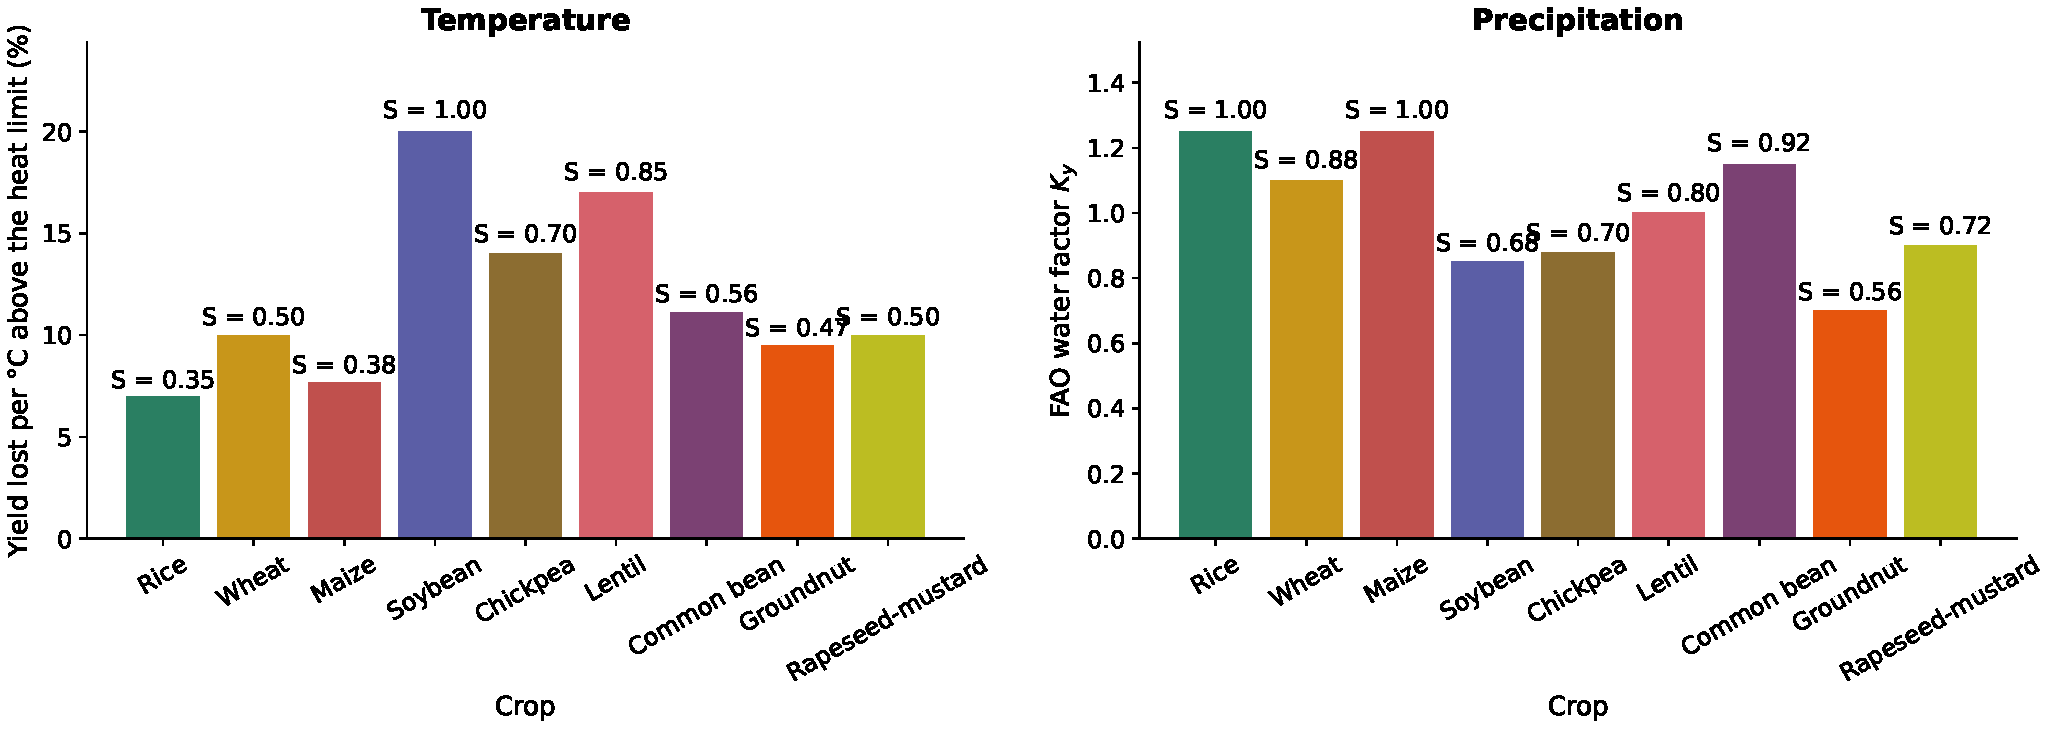
\includegraphics[width=0.85\linewidth]{F05l_literature_sensitivity.pdf}
\caption{Literature sensitivity of the nine crops: heat slope and $K_y$.}\label{fig:litsens}\end{figure}

\begin{figure}[H]\centering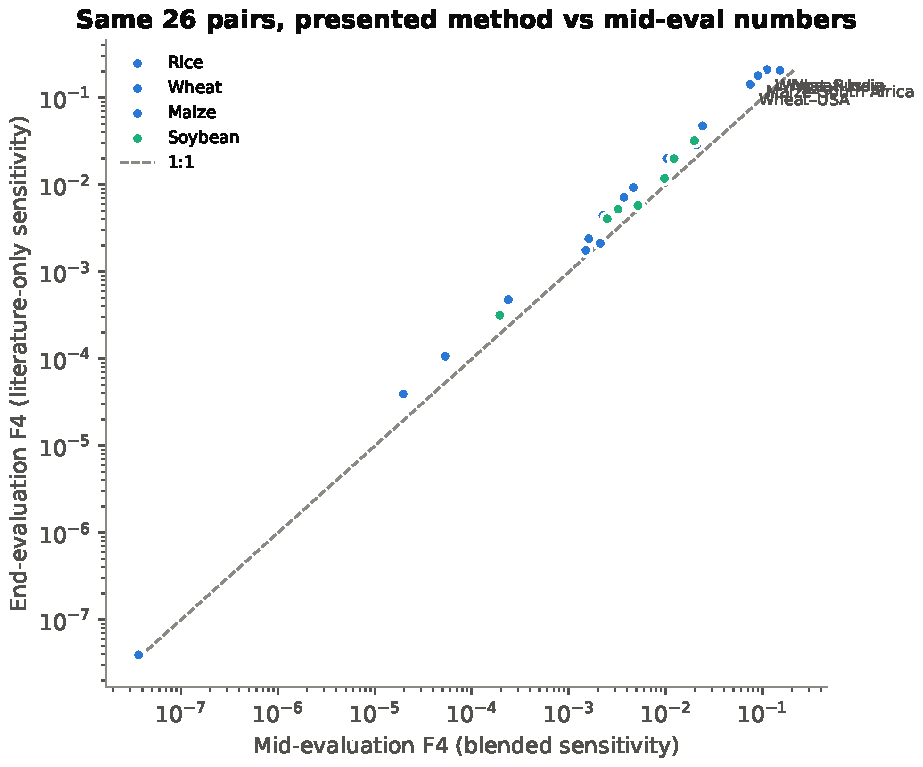
\includegraphics[width=0.6\linewidth]{G11_mideval_vs_literature_only.pdf}
\caption{The same 26 pairs: frozen mid-evaluation values (blended sensitivity) against the presented
literature-only method.}\label{fig:midlit}\end{figure}

\begin{table}[H]\centering\small\caption{Food-supply diversity (effective number of FBS items supplying each
nutrient, 2021--23) and share of supply from the nine crops.}\label{tab:diversity}
\adjustbox{max width=\linewidth}{\begin{tabular}{lrrrrrlrr}
\toprule
Country & kcal & protein & Zn & Fe & cereal \% kcal & top iron source & 9 crops \% kcal & 9 crops \% Fe \\
\midrule
Bangladesh & 5.9 & 8.0 & 6.9 & 10.7 & 68 & Rice and products & 74 & 53 \\
Myanmar & 8.0 & 10.2 & 8.6 & 13.5 & 62 & Rice and products & 70 & 47 \\
Egypt & 12.1 & 10.8 & 7.5 & 8.8 & 62 & Wheat and products & 65 & 68 \\
Ethiopia & 14.0 & 12.1 & 10.8 & 12.1 & 54 & Wheat and products & 43 & 46 \\
India & 16.1 & 12.8 & 11.6 & 13.8 & 51 & Wheat and products & 58 & 56 \\
Russian Federation & 16.8 & 12.5 & 10.1 & 10.2 & 33 & Wheat and products & 33 & 51 \\
South Africa & 16.9 & 11.6 & 9.8 & 10.2 & 43 & Maize and products & 48 & 65 \\
United Republic of Tanzania & 17.0 & 15.5 & 12.6 & 12.4 & 45 & Maize and products & 51 & 67 \\
Türkiye & 17.4 & 11.9 & 9.7 & 11.5 & 37 & Wheat and products & 40 & 53 \\
Ukraine & 17.6 & 13.7 & 11.3 & 11.0 & 34 & Wheat and products & 32 & 46 \\
Argentina & 17.9 & 11.7 & 9.7 & 11.2 & 31 & Wheat and products & 35 & 54 \\
China, mainland & 19.1 & 16.6 & 15.1 & 14.2 & 46 & Vegetables, other & 52 & 39 \\
Nigeria & 19.6 & 19.8 & 17.1 & 17.7 & 37 & Sorghum and products & 33 & 34 \\
Italy & 20.8 & 12.9 & 10.5 & 12.0 & 28 & Wheat and products & 32 & 49 \\
United States of America & 22.6 & 13.5 & 14.6 & 18.1 & 21 & Wheat and products & 37 & 40 \\
Brazil & 22.8 & 13.4 & 13.9 & 16.5 & 27 & Wheat and products & 39 & 51 \\
Belarus & 23.0 & 14.4 & 14.4 & 14.4 & 24 & Wheat and products & 21 & 28 \\
France & 23.8 & 13.9 & 13.3 & 15.3 & 26 & Wheat and products & 29 & 43 \\
Australia & 24.8 & 15.9 & 14.8 & 17.1 & 20 & Wheat and products & 31 & 39 \\
Canada & 25.4 & 17.3 & 16.2 & 18.9 & 24 & Wheat and products & 36 & 44 \\
World & 26.9 & 20.8 & 18.3 & 21.2 & 42 & Wheat and products & -- & -- \\
\bottomrule
\end{tabular}
}\end{table}

\clearpage
\section{Record of corrections}\label{app:corrections}
Table~\ref{tab:corrections} lists every error found after the first end-evaluation version and how it was fixed.
Decisions E18 and E19 are recorded in \file{docs/DECISION\_REGISTER\_END\_EVAL.md}.

{\small
\begin{longtable}{p{0.4cm}p{4.6cm}p{5.0cm}p{4.6cm}}
\caption{Corrections made during the end-evaluation audits.}\label{tab:corrections}\\
\toprule
& Issue & Fix & Effect on results \\
\midrule\endfirsthead
\toprule & Issue & Fix & Effect on results \\ \midrule\endhead
\bottomrule\endfoot
1 & The nine-crop supply share counted only crops with an FBS item of their own, omitting chickpea and lentil. & Numerator from summed crop contributions (SUA for chickpea and lentil), denominator FBS total; World left blank (no SUA); not added to totals or to the Shannon items (E18). & India: energy \shareOldKcal\ $\to$ \shareNewKcal\%, protein \shareOldProtein\ $\to$ \shareNewProtein\%, iron \shareOldIron\ $\to$ \shareNewIron\%, zinc \shareOldZinc\ $\to$ \shareNewZinc\%. No index value changes. \\
2 & Yield-to-nutrient bounds: Canada lentil has negative 2023 domestic supply in FAOSTAT (residuals $-$267\,kt), so SSR $<0$ turned a loss into a gain; in five pairs the lower bound exceeded the upper. & SSR capped to [0,1], non-positive supply with positive production counted as SSR = 1, lower bound $\le$ upper bound, in both historical and future accounting (E19). & 7 historical scenario rows and 3 future rows changed by at most 0.26 percentage points of a nutrient; no ranking or headline value changed. \\
3 & Committed four-crop outputs (empirical sensitivity, S1/S2 scenarios) were stale, i.e.\ not what the code produces. & Regenerated; now identical to the nine-crop run on the 24 shared pairs. & Empirical water slope differed by up to 33, S1/S2 yield changes by up to 20 points; checks only, so no main index value changed. \\
4 & Derived heat parameters were fitted in an unsaved scratch script. & \file{code/25\_parameter\_fits.py} refits them from the tabulated published data (a bounded optimiser hit local minima; replaced by a grid). & Reproduces \file{config.py} to its rounding; no value changed. \\
5 & The raw-data manifest did not list the 19 Telangana-mask and Indian survey files used by the analysis. & Added with checksums, existing rows unchanged. & None. \\
6 & The pipeline did not stop on a failed document compile; no automated arithmetic checks. & Compile exit codes checked; \file{24\_checks.py} runs before the documents. & None. \\
7 & Text said wheat's future increase in the USA is water-driven, and bean has no empirical response in ``most'' countries. & Checked against \file{future\_components.csv} and \file{future\_yield.csv}: USA is shared heat/water; bean has no detected response in any country. & Wording only. \\
8 & Rice $K_y$: FAO-33's rice chapter is at p.~125 and gives no number (rice is classed ``high''). & Proxy label made explicit. & None. \\
9 & Reference: Beach et al.\ (2019) had been cited as ``Smith and Myers 2019''. & Corrected in \file{refs.bib}. & Reference [16] of the submitted literature review still carries the wrong authorship. \\
10 & Layout: a future table ran 174\,pt past the margin; notes shrank tables; overlapping tick labels in a figure. & Tables wrapped and notes set under the table; tick formatter fixed. & None. \\
\end{longtable}}

\clearpage
\section{Audit evidence}\label{app:audit}
{\scriptsize\begin{longtable}{rL{0.569}cL{0.261}}
\caption[Consistency checks run on the saved results]{Consistency checks run on the saved results.}\label{tab:checks}\\
\toprule
 & Check (\texttt{code/24\_checks.py}) & Result & Detail \\
\midrule\endfirsthead
\toprule
 & Check (\texttt{code/24\_checks.py}) & Result & Detail \\
\midrule\endhead
\bottomrule\endfoot
1 & nine crops in panels & pass & 9 crops, 59 pairs \\
2 & every crop appears in docs/input\_register.csv & pass & [] \\
3 & E\_heat = observed level / fixed maximum & pass & max 5.0463 \\
4 & E\_water = observed level / fixed maximum & pass & max 0.7894 \\
5 & index\_reference maxima equal component maxima & pass &  \\
6 & S\_heat is literature slope / max slope (literature-only) & pass &  \\
7 & S\_water is FAO K\_y / max K\_y (literature-only) & pass &  \\
8 & I = mean of five nutrient shares & pass &  \\
9 & In = I / max I & pass &  \\
10 & F4 recomputed from components & pass &  \\
11 & crop score, equal weights = mean over countries & pass &  \\
12 & crop score, production weights & pass &  \\
13 & group score = simple mean of its three crop scores & pass &  \\
14 & future run's 'present' column reproduces the main F4 & pass &  \\
15 & historical\_1971\_2000: E uses the FIXED present-period maximum & pass &  \\
16 & future\_2041\_2060: E uses the FIXED present-period maximum & pass &  \\
17 & S and In identical across periods & pass &  \\
18 & dF4 = heat part + water part & pass &  \\
19 & 1971-2000 comparator reproduces main series (relative < 1e-3) & pass & max rel 1.94e-07 \\
20 & yield change comes from loss accounting, not from index values & pass &  \\
21 & crop\_contrib national totals equal the adequacy (FBS) totals & pass & 2848 country-years \\
22 & nine crops never exceed 100\% of any national nutrient supply & pass & max 0.835 \\
23 & SUA chickpea+lentil kcal do not exceed the FBS 'Pulses, Other' aggregate (5\% tolerance) & pass & 0.1\% of 2369 country-years exceed (SUA and FBS can differ) \\
24 & SUA rows are labelled and kept out of national totals & pass &  \\
25 & India nine-crop share (diversity table) = summed crop contributions & pass & kcal 0.5800 vs 0.5800 \\
26 & nine-crop share >= FBS-item-only share everywhere it is defined & pass &  \\
27 & standard shock is -10\% everywhere & pass &  \\
28 & historical scenarios: supply changes are <= 0 and the lower bound is no larger than the upper bound & pass &  \\
29 & future nutrition: supply changes are <= 0 and the lower bound is no larger than the upper bound & pass &  \\
\end{longtable}}


{\scriptsize\begin{longtable}{L{0.250}L{0.381}L{0.113}rrr}
\caption[Outputs that are not identical in both runs: new outputs of this audit, and previous files the pipeline no longer writes]{Outputs that are not identical in both runs: new outputs of this audit, and previous files the pipeline no longer writes. No file present in both runs differs.}\label{tab:auditdiff}\\
\toprule
Area & File (* = each crop) & Status & Files & max abs & max rel \\
\midrule\endfirsthead
\toprule
Area & File (* = each crop) & Status & Files & max abs & max rel \\
\midrule\endhead
\bottomrule\endfoot
\file{work} & \file{\_qcl\_prod\_2020\_24.pkl} & missing & 1 &  &  \\
\file{work} & \file{\_sua\_pulses.pkl} & missing & 1 &  &  \\
\file{work} & \file{metrics\_prec\_*\_annual.npz} & missing & 12 &  &  \\
\file{work} & \file{metrics\_prec\_*\_flow.npz} & missing & 12 &  &  \\
\file{work} & \file{metrics\_prec\_*\_gs.npz} & missing & 12 &  &  \\
\file{work} & \file{metrics\_tmax\_*\_annual.npz} & missing & 12 &  &  \\
\file{work} & \file{metrics\_tmax\_*\_flow.npz} & missing & 12 &  &  \\
\file{work} & \file{metrics\_tmax\_*\_gs.npz} & missing & 12 &  &  \\
\file{work} & \file{run\_chain.sh} & missing & 1 &  &  \\
\file{processed} & \file{nine\_crop/parameter\_fits.csv} & new & 1 &  &  \\
\file{docs/nine\_crop/generated} & \file{numbers\_report.tex} & new & 1 &  &  \\
\file{docs/nine\_crop/generated} & \file{tab\_audit\_diff.tex} & new & 1 &  &  \\
\file{docs/nine\_crop/generated} & \file{tab\_audit\_summary.tex} & new & 1 &  &  \\
\file{docs/nine\_crop/generated} & \file{tab\_checks.tex} & new & 1 &  &  \\
\file{docs/nine\_crop/generated} & \file{tab\_crop\_mapping.tex} & new & 1 &  &  \\
\file{docs/nine\_crop/generated} & \file{tab\_data\_sources.tex} & new & 1 &  &  \\
\file{docs/nine\_crop/generated} & \file{tab\_diversity.tex} & new & 1 &  &  \\
\file{docs/nine\_crop/generated} & \file{tab\_fits.tex} & new & 1 &  &  \\
\file{docs/nine\_crop/generated} & \file{tab\_india\_shares.tex} & new & 1 &  &  \\
\file{docs/nine\_crop/generated} & \file{tab\_india\_sources.tex} & new & 1 &  &  \\
\file{docs/nine\_crop/generated} & \file{tab\_ledger.tex} & new & 1 &  &  \\
\end{longtable}}


\section{India, Telangana and Hyderabad sources}\label{app:indiasources}
Every number used in Section~\ref{sec:india} is stored once with its table or page in
\file{data/external/india\_hyderabad\_indicators.csv}. The source register \file{docs/india\_hyderabad\_sources.md} is
generated from that file. Table~\ref{tab:indiasources} summarises it.

{\scriptsize\begin{longtable}{L{0.140}L{0.343}L{0.330}rL{0.102}}
\caption[Official sources of the India/Telangana/Hyderabad analysis]{Official sources of the India/Telangana/Hyderabad analysis (from \texttt{data/external/india\_hyderabad\_indicators.csv}).}\label{tab:indiasources}\\
\toprule
Source & Citation & Granularity and use & Rows & Read level \\
\midrule\endfirsthead
\toprule
Source & Citation & Granularity and use & Rows & Read level \\
\midrule\endhead
\bottomrule\endfoot
\file{NFHS5\_TG\_FS} & IIPS \& ICF (2020/2021). National Family Health Survey (NFHS-5) 2019-21, State Fact Sheet: Telangana (Key Indicators). Mumbai: IIPS; Ministry of Health and Family Welfare, Govt of India. & NFHS-5 Telangana state fact sheet (urban, rural, total; NFHS-4 for trend). & 76 & table read \\
\file{NFHS5\_IN\_FS} & IIPS \& ICF (2020). National Family Health Survey (NFHS)-5, India and State Factsheet Compendium (Phase II). Mumbai: IIPS. & NFHS-5 India key indicators (comparison). & 76 & table read \\
\file{NFHS5\_TG\_REP} & International Institute for Population Sciences (IIPS) and ICF. 2021. National Family Health Survey (NFHS-5), India, 2019-21: Telangana. Mumbai: IIPS. & NFHS-5 Telangana state report: food-frequency tables for women and men 15-49, child feeding, anaemia. & 101 & table read \\
\file{NFHS5\_HYD\_DFS} & IIPS / MoHFW. India Districts Factsheets of National Family Health Survey (NFHS)-5, 2019-2021 (district fact sheet values), published on Open Government Data Platform India (data.gov.in), resource cf80173e-fece-439d-a0b1-6e9cb510593d; record District=Hyderabad, State=Telangana. & NFHS-5 Hyderabad DISTRICT fact sheet (fully urban) via the official data.gov.in API. Values printed in parentheses or as * in the source are small-sample and are not used. & 17 & table read (official open-data copy of district fact sheet) \\
\file{CNNS\_TG\_FS} & Ministry of Health and Family Welfare (MoHFW), UNICEF and Population Council. 2019. Comprehensive National Nutrition Survey (CNNS) 2016-18, Telangana Factsheet. New Delhi. & CNNS 2016-18 Telangana fact sheet: serum ferritin, zinc, anaemia, vitamins (children 1-4, 5-9, adolescents 10-19). & 55 & table read \\
\file{CNNS\_NAT} & Ministry of Health and Family Welfare (MoHFW), Government of India, UNICEF and Population Council. 2019. Comprehensive National Nutrition Survey (CNNS) National Report. New Delhi. & CNNS 2016-18 national report tables. & 92 & table read, table read (text layer), table read (text layer, verified against page image for Table 4.5) \\
\file{NSS594} & National Statistics Office, MoSPI, Govt of India. 2025. Nutritional Intake in India (2022-23 \& 2023-24), NSS Report No. 594 (HCES: 2022-23 \& 2023-24). & State x rural/urban nutrient intake (energy, protein, fat) and food-group shares, 2022-23 and 2023-24. & 112 & table read \\
\file{NSS592} & National Statistics Office, MoSPI, Govt of India. 2025. Survey on Household Consumption Expenditure: 2023-24, NSS Report No. 592 (HCES: 2023-24). & State x rural/urban HCES 2023-24 report tables (expenditure shares). & 64 & table read \\
\file{HCES2324\_A10S} & National Statistics Office, MoSPI. HCES 2023-24 (NSS Report No. 592), Appendix Table A10S: Monthly per capita quantity and value of consumption at detailed item level for all items of consumption by State/UT and All-India (Excel). & State x rural/urban household consumption (quantity and value per person per 30 days). Not city-level: Telangana urban is the nearest description of Hyderabad. & 465 & table read \\
\file{TG\_DES\_AAG2024} & Directorate of Economics and Statistics, Government of Telangana. 2024. Telangana State At A Glance 2024. Hyderabad. & Telangana Directorate of Economics and Statistics, At a Glance 2024: crop area and production 2023-24 (provisional), rainfall. & 108 & table read \\
\file{TG\_SEO2025} & Planning Department, Government of Telangana. 2025. Telangana Socio Economic Outlook 2025 (data source: Directorate of Economics and Statistics, Telangana). & Telangana Socio-Economic Outlook 2025: yields, rainfall, net area sown. & 41 & figure data labels read, table read \\
\file{NNMB\_URBAN} & National Nutrition Monitoring Bureau (NNMB), ICMR-National Institute of Nutrition. 2017. Diet and Nutritional Status of Urban Population in India and Prevalence of Obesity, Hypertension, Diabetes and Hyperlipidemia in Urban Men and Women - A brief NNMB Urban Nutrition Report. Hyderabad: NIN. & ICMR-NIN NNMB urban brief report: pooled urban India (16 states); Telangana is NOT included, so it is not used for Hyderabad. & 18 & figure data labels read (scanned report) \\
\file{IFCT2017} & Longvah, T., Ananthan, R., Bhaskarachary, K. and Venkaiah, K. (2017). Indian Food Composition Tables 2017. National Institute of Nutrition (ICMR), Hyderabad, Telangana, India. & ICMR-NIN Indian Food Composition Tables 2017, Table 5 (iron, zinc; mg per 100 g edible portion, raw foods). & 44 & table read \\
\end{longtable}}


\end{document}
